\documentclass[a4paper,11pt,twoside]{book}

%pacchetti

\usepackage[english]{babel}
\usepackage{appendix}
\usepackage{amsmath,amssymb,amscd,amsthm}
\usepackage{dsfont}
\usepackage{bbm}
%\usepackage{hyperref}
\usepackage{stmaryrd}
\usepackage{enumitem}
%\usepackage{yfonts}
\usepackage[T1]{fontenc}
\usepackage[utf8x]{inputenc}
%\usepackage{enumerate}
\usepackage{verbatim}
\usepackage{graphicx}
\usepackage{faktor}
\usepackage[table]{xcolor}
\usepackage{xfrac}
\usepackage{tikz,tikz-cd}
\usetikzlibrary{arrows,decorations.pathmorphing,decorations.pathreplacing,patterns}
\usepackage[all]{xy}
\usepackage{tabularx}
\usepackage{longtable}
\usepackage{tabu}
\usepackage{booktabs}
\usepackage{mathtools}
\usepackage{mathrsfs}
\usepackage[alphabetic,initials]{amsrefs}

%\usepackage{fix-cm}
%\usepackage{caption}
%\captionsetup{format=hang}
%\usepackage{subcaption}
%\usepackage{keyval}
%\usepackage[lofdepth,lotdepth]{subfig}
%\usepackage[10pt]{type1ec} %per avere i caratteri greci non bitmapped

\usepackage{setspace} %pacchetto per l'interlinea
\onehalfspacing %interlinea 1.5

%MARGINI
\usepackage{geometry} %per i margini
\geometry{a4paper, top=3cm, bottom=3cm, left=3cm, right=3cm} %bindingoffset e' per la rilegatura

%INTESTAZIONI
\usepackage{fancyhdr}
\pagestyle{fancy}
\renewcommand{\headrulewidth}{0pt}
\fancyhf{}
\fancyhead[LE,RO]{\small \thepage} %mette il numero di pagina in grassetto e carattere piccolo nelle intestazioni a sinistra nelle pagine even e a destra nelle pagine odd
\fancyhead[CE]{\small  \raggedleft \nouppercase{\leftmark}}
\fancyhead[CO]{\small  \raggedright \nouppercase{\rightmark}}
%\scshape

%\fancypagestyle{plain}{%
%\fancyhf{}\fancyfoot[C]{\small \thepage}} %modifica lo stile plain che e' quello dell'apertura dei capitoli


%dobbiamo dirgli di fare la pagina bianca, senza intestazioni quando finisce un capitolo
\makeatletter
\def\cleardoublepage{\clearpage\if@twoside \ifodd\c@page\else
\hbox{}
\vspace*{\fill}
\vspace{\fill}
\thispagestyle{empty}
\newpage
\if@twocolumn\hbox{}\newpage\fi\fi\fi}
\makeatother

%%%%%%%%%%%%%%%%
%controllo dei titoli
\usepackage{titlesec}
\titleformat{\section}[block]{\normalfont\large\bfseries}{\S\ \thesection.}{1em}{}[]
\titleformat{\subsection}[runin]{\normalfont\bfseries}{\thetitle.}{.5em}{}[.]
%\titlelabel{\thetitle. } %etichetta prima del nome del titolo. \thetitle dovrebbe essere il numero

%CHAPTER

\usepackage[Glenn]{fncychap}
%\newcommand{\chapnumfont}{%     % define font for chapter number
%  \usefont{T1}{pnc}{b}{n}%      % choose New Chancery, bold, normal shape
%  \fontsize{100}{100}%          % font size 100pt, baselineskip 100pt
%  \selectfont%                  % activate font
%}
%\colorlet{chapnumcol}{gray!75}  % color for chapter number

%\titleformat{\chapter}[display]
%{\filleft\bfseries}
%{\filleft\chapnumfont\textcolor{chapnumcol}{\thechapter}}
%{-24pt}
%{\Huge}





%%%%%%%%%%%%%%%%%%%%%%%%

%\usepackage{comment}
\usepackage{stackrel}

\usepackage[colorlinks=false,  pdftex,   pdfpagemode=UseOutlines]{hyperref} %collegamenti interni

%\usepackage{tabularx}
%\usepackage{booktabs}
%\usepackage{longtable}
%\usepackage{colortbl}
%\definecolor{light-gray}{gray}{0.85}

%\usepackage{rotating}

%comandi

\newcommand{\ilemph}[1]{\emph{#1}}
\newcommand{\pazocal}{\mathcal}
\newcommand{\plC}{\scalebox{0.8}[1.3]{$\sqsubset$}}
\newcommand{\TT}{\operatorname{T}}
\newcommand{\oM}{\overline{\mathcal{M}}}
\newcommand{\tM}{\widetilde{\mathcal{M}}}
\newcommand{\M}[4]{\overline{\mathcal{M}}_{#1,#2}(#3,#4)}
\newcommand{\MK}[4]{\overline{\mathcal{M}}^{\rm{Kim}}_{#1,#2}(#3,#4)}
\newcommand{\Mone}[3]{\overline{\pazocal M}^{(1)}_{1,#1}(#2,#3)}
\newcommand{\VZ}[3]{\mathcal{V\!Z}_{1,#1}(#2,#3)}
\newcommand{\VZK}[3]{\mathcal{V\!Z}^{\rm{Kim}}_{1,#1}(#2,#3)}
\newcommand{\VZa}[3]{\mathcal{V\!Z}^{\rm{ACGS}}_{1,#1}(#2,#3)}
\newcommand{\VZdrc}[3]{\mathcal{V\!Z}^{\rm{DRC}}_{1,#1}(#2,#3)}
\newcommand{\tVZ}[3]{\widetilde{\mathcal{V\!Z}}_{1,#1}(#2,#3)}
\newcommand{\Zp}{\pazocal Z^p}
\newcommand{\tZ}{\widetilde{\pazocal Z}}
\newcommand{\tZp}{\widetilde{\pazocal Z}^p}
\newcommand{\oZp}{\overline{\mathcal Z}^{p,\rm{gst}}}
\newcommand{\XP}{\mathfrak Z}
\newcommand{\tXP}{\widetilde{\mathfrak Z}}
\newcommand{\Q}[4]{\mathcal{Q}_{#1,#2}(#3,#4)}
\newcommand{\Qe}[4]{\mathcal{Q}^{\epsilon}_{#1,#2}(#3,#4)}
\newcommand{\Qt}[4]{\widetilde{\mathcal Q}_{#1,#2}(#3,#4)}
\newcommand{\QG}[4]{\mathcal{QG}_{#1,#2}(#3,#4)}
\newcommand{\QGe}[4]{\mathcal{QG}^{\epsilon}_{#1,#2}(#3,#4)}
\newcommand{\PP}{\mathbb P}
\newcommand{\QQ}{\mathbb{Q}}
\newcommand{\Z}{\mathbb{Z}}
\newcommand{\N}{\mathbb{N}}
\newcommand{\OO}{\mathcal{O}}
\renewcommand{\to}{\rightarrow}
\newcommand{\A}{\mathcal A}
\newcommand{\B}{\mathcal B}
\newcommand{\C}{\mathfrak C}
\newcommand{\F}{\mathcal F}
\newcommand{\EE}{\mathbf{E}}
\renewcommand{\L}{\mathcal L}
\newcommand{\LL}{\mathbf{L}}
\newcommand{\pM}{\pazocal M}
\newcommand{\MM}{\mathfrak M}
\newcommand{\Mwt}{\mathfrak M_1^{\textrm{wt}}}
\newcommand{\Aaff}{\mathbb{A}}
\newcommand{\kk}{\Bbbk}
\newcommand{\comp}{\chi}
\newcommand{\sst}{\sigma^{\operatorname{ss}}}
\newcommand{\Pic}{\operatorname{Pic}}
\newcommand{\Def}{\operatorname{Def}}
\newcommand{\Spec}{\operatorname{Spec}}
\newcommand{\Proj}{\operatorname{Proj}}
\newcommand{\Hom}{\operatorname{Hom}}
\newcommand{\Ext}{\operatorname{Ext}}
\newcommand{\val}{\operatorname{val}}
\newcommand{\Gm}{\mathbb{G}_{\text{m}}}
\newcommand{\virt}[1]{[#1]^{\mathrm{vir}}}
\newcommand{\virloc}[1]{[#1]^{\mathrm{vir}}_{\mathrm{loc}}}
\newcommand{\vip}[1]{[#1]^{\operatorname{prod}}}
\newcommand{\redu}[1]{[#1]^{\operatorname{red}}}
\newcommand{\Id}{\operatorname{Id}}
\newcommand{\CC}{\mathbb{C}}
\newcommand{\ZZ}{\mathbb{Z}}
\newcommand{\HH}{\operatorname{H}}
\newcommand{\Achow}{\operatorname{A}}
\newcommand{\pt}{\operatorname{pt}}
\newcommand{\m}{\mathfrak m}
\newcommand{\tR}{\widetilde{R}}
\newcommand{\tm}{\widetilde{\mathfrak m}}
\newcommand{\lala}{\langle\!\langle}
\newcommand{\rara}{\rangle\!\rangle}
\newcommand{\bq}{\begin{equation}}
\newcommand{\eq}{\end{equation}}
\newcommand{\ba}{\begin{aligned}}
\newcommand{\ea}{\end{aligned}}
\newcommand{\be}{\begin{enumerate}}
\newcommand{\ee}{\end{enumerate}}
\newcommand{\bsm}{\left(\begin{smallmatrix}}
\newcommand{\esm}{\end{smallmatrix}\right)}                   
\newcommand{\bpm}{\begin{pmatrix}}
\newcommand{\epm}{\end{pmatrix}}
\newcommand{\barr}{\begin{displaymath}\begin{array}{cccc}}
\newcommand{\earr}{\end{array}\end{displaymath}}
\newcommand{\barrl}{\begin{displaymath}\begin{array}{lcl}}
\newcommand{\earrl}{\end{array}\end{displaymath}}
\newcommand{\barl}{\begin{displaymath}\begin{array}{l}}
\newcommand{\earl}{\end{array}\end{displaymath}}
\newcommand{\bxym}{ \begin{displaymath}\xymatrix }
\newcommand{\exym}{\end{displaymath}}
\newcommand{\bcd}{\begin{center}\begin{tikzcd}}
\newcommand{\ecd}{\end{tikzcd}\end{center}}
\newcommand{\R}{\operatorname{R}^{\bullet}}
%\newcommand{\sslash}{\mathbin{/\mkern-6mu/}}
\newcommand{\tr}{{\rm tr}}
\newcommand{\Isom}{\text{Isom}}
\newcommand{\pr}{\operatorname{pr}}
\newcommand{\fgt}{\operatorname{fgt}}
\newcommand{\ev}{\operatorname{ev}}
\newcommand{\codim}{\operatorname{codim}}
\newcommand{\rk}{\operatorname{rk}}
\newcommand{\vdim}{\operatorname{vdim}}
\newcommand{\Bl}{\operatorname{Bl}}
\newcommand{\ildef}[1]{\emph{#1}}
\newcommand{\om}[1]{\mathcal{#1}}
\newcommand{\h}{\operatorname{h}}
\newcommand{\vv}{\operatorname{v}}
\newcommand{\Aut}{\operatorname{Aut}}
\newcommand{\RR}{\mathbb{R}}
\newcommand{\NN}{\operatorname{N}}
\newcommand{\id}{\mathrm{id}}
\newcommand{\dvr}{\Delta}
\newcommand{\cC}{\mathcal{C}}
\newcommand{\hC}{\overline{\mathcal{C}}}
\newcommand{\hP}{\overline{\mathfrak{P}}}
\newcommand{\hL}{\overline{\mathcal{L}}}
\newcommand{\w}{\mathbf{w}}

%figurine

\def\reduced{\tikz[baseline=-3pt]{
\draw (0,0) circle[radius=2pt]}
}
\def\Dunouno{\tikz[baseline=-3pt]{
\draw (0,0)node[above]{$\psi$} -- (1,0)node[above]{$H$};
\draw (0,0) circle(2pt)[fill=white];
\fill (1,0) circle (2pt)}
}
\def\Dunodue{\tikz[baseline=-3pt]{
\draw (0,0)-- (1,0)node[above]{$\psi H$};
\draw (0,0) circle(2pt)[fill=white];
\fill (1,0) circle (2pt)}
}
\def\Dunotre{\tikz[baseline=-3pt]{
\draw (0,0)node[above]{$\lambda_1\psi$} -- (1,0);
\draw (0,0) circle(2pt)[fill=white];
\fill (1,0) circle (2pt)}
}
\def\Dunoquat{\tikz[baseline=-3pt]{
\draw (0,0)node[above]{$\lambda_1$} -- (1,0)node[above]{$\psi$};
\draw (0,0) circle(2pt)[fill=white];
\fill (1,0) circle (2pt)}
}
\def\Dunocin{\tikz[baseline=-3pt]{
\draw (0,0)node[above]{$\psi^2$} -- (1,0);
\draw (0,0) circle(2pt)[fill=white];
\fill (1,0) circle (2pt)}
}
\def\Dunosei{\tikz[baseline=-3pt]{
\draw (0,0)node[above]{$\psi$} -- (1,0)node[above]{$\psi$};
\draw (0,0) circle(2pt)[fill=white];
\fill (1,0) circle (2pt)}
}
\def\Dunoset{\tikz[baseline=-3pt]{
\draw (0,0) -- (1,0)node[above]{$\psi^2$};
\draw (0,0) circle(2pt)[fill=white];
\fill (1,0) circle (2pt)}
}
\def\Dunoott{\tikz[baseline=-3pt]{
\draw (0,0)node[above]{$\lambda_1^2$} -- (1,0);
\draw (0,0) circle(2pt)[fill=white];
\fill (1,0) circle (2pt)}
}
\def\Dunonov{\tikz[baseline=-3pt]{
\draw (0,0)node[above]{$\lambda_1$} -- (1,0)node[above]{$H$};
\draw (0,0) circle(2pt)[fill=white];
\fill (1,0) circle (2pt)}
}
\def\Dunodiec{\tikz[baseline=-3pt]{
\draw (0,0) -- (1,0)node[above]{$H^2$};
\draw (0,0) circle(2pt)[fill=white];
\fill (1,0) circle (2pt)}
}
\def\Ddueuno{\tikz[baseline=-3pt]{
\draw (0,0) -- (1,.3)node[above]{$H$} (0,0)--(1,-.3);
\draw (0,0) circle(2pt)[fill=white];
\fill (1,.3) circle (2pt) (1,-.3) circle (2pt)}
}
\def\Dduedue{\tikz[baseline=-3pt]{
\draw (0,0)node[above]{$\lambda_1$} -- (1,.3) (0,0)--(1,-.3);
\draw (0,0) circle(2pt)[fill=white];
\fill (1,.3) circle (2pt) (1,-.3) circle (2pt)}
}
\def\Dduetre{\tikz[baseline=-3pt]{
\draw (0,0)node[above]{$\psi$} -- (1,.3) (0,0)--(1,-.3);
\draw (0,0) circle(2pt)[fill=white];
\fill (1,.3) circle (2pt) (1,-.3) circle (2pt)}
}
\def\Dduequat{\tikz[baseline=-3pt]{
\draw (0,0)node[below]{$\psi$} -- (1,.3) (0,0)--(1,-.3);
\draw (0,0) circle(2pt)[fill=white];
\fill (1,.3) circle (2pt) (1,-.3) circle (2pt)}
}
\def\Dduecin{\tikz[baseline=-3pt]{
\draw (0,0) -- (1,.3)node[above]{$\psi$} (0,0)--(1,-.3);
\draw (0,0) circle(2pt)[fill=white];
\fill (1,.3) circle (2pt) (1,-.3) circle (2pt)}
}
\def\Dduesei{\tikz[baseline=-3pt]{
\draw (0,0) -- (1,.3) (0,0)--(1,-.3)node[below]{$\psi$};
\draw (0,0) circle(2pt)[fill=white];
\fill (1,.3) circle (2pt) (1,-.3) circle (2pt)}
}
\def\Dtre{\tikz[baseline=-3pt]{
\draw (0,0) -- (1,.5) (0,0)--(1,-.5) (0,0) -- (1.3,0);
\draw (0,0) circle(2pt)[fill=white];
\fill (1,.5) circle (2pt) (1,-.5) circle (2pt) (1.3,0) circle (2pt)}
}

\def\Dk{\tikz[baseline=-3pt]{
\draw (0,0)node[left]{\scriptsize $g=2,d=0$} -- (1,.5) node[right]{\scriptsize $g=0,d_1$} (0,0)--(1,-.5)node[right]{\scriptsize $g=0,d_k$} (0,0) -- (1.2,.2)node[right]{\scriptsize $g=0,d_2$};
\draw (1.2,-.2) node[right]{\scriptsize $\ldots$};
\draw (0,0) circle(2pt)[fill=white];
\fill (1,.5) circle (2pt) (1,-.5) circle (2pt) (1.2,.2) circle (2pt)}
}

\def\Ek{\tikz[baseline=-3pt]{
\draw (-1.5,0) node[left]{\scriptsize $g=1,d_0$} -- (0,0);
\draw (0,0)node[above]{\scriptsize \begin{tabular}{c} $g=1,$ \\ $d=0$ \end{tabular}} -- (1,.5) node[right]{\scriptsize $g=0,d_1$} (0,0)--(1,-.5)node[right]{\scriptsize $g=0,d_k$} (0,0) -- (1.2,.2)node[right]{\scriptsize $g=0,d_2$};
\draw (1.2,-.2) node[right]{\scriptsize $\ldots$};
\draw (0,0) circle(2pt)[fill=white];
\fill (-1.5,0) circle (2pt) (1,.5) circle (2pt) (1,-.5) circle (2pt) (1.2,.2) circle (2pt)}
}

\def\Ekk{\tikz[baseline=-3pt]{
\draw (-3,0)node[above]{\scriptsize \begin{tabular}{c} $g=1,$ \\ $d=0$ \end{tabular}} -- (-4,.5) node[left]{\scriptsize $g=0,d_{1,1}$} (-3,0)--(-4,-.5)node[left]{\scriptsize $g=0,d_{1,k_1}$} (-3,0) -- (-4.2,.2)node[left]{\scriptsize $g=0,d_{1,2}$};
\draw (-3,0) -- (-1.5,0) node[below]{\scriptsize $g=0,d_0$} -- (0,0);
\draw (0,0)node[above]{\scriptsize \begin{tabular}{c} $g=1,$ \\ $d=0$ \end{tabular}} -- (1,.5) node[right]{\scriptsize $g=0,d_{2,1}$} (0,0)--(1,-.5)node[right]{\scriptsize $g=0,d_{2,k_2}$} (0,0) -- (1.2,.2)node[right]{\scriptsize $g=0,d_{2,2}$};
\draw (1.2,-.2) node[right]{\scriptsize $\ldots$} (-4.2,-.2) node[right]{\scriptsize $\ldots$};
\draw (0,0) circle(2pt)[fill=white] (-3,0) circle(2pt)[fill=white];
\fill (-1.5,0) circle (2pt) (1,.5) circle (2pt) (1,-.5) circle (2pt) (1.2,.2) circle (2pt) (-4,.5) circle (2pt) (-4,-.5) circle (2pt) (-4.2,.2) circle (2pt)}
}

\def\pacman{\tikz[baseline=-3pt]{
\draw (0,0)node[left]{\scriptsize $g=0,d$} to[out=20,in=160] (1,0) node[right]{\scriptsize $g=1,d=0$};
\draw (0,0) to[out=-20,in=-160] (1,0);
\fill (0,0) circle (2pt);
\draw[fill=white] (1,0) circle (2pt)}
}

\def\hypell{\tikz[baseline=-3pt]{
\draw (0,0)node[left]{\scriptsize $g=2,d_0=2$} -- (1,.5) node[right]{\scriptsize $g=0,\bar d_1$} (0,0)--(1,-.5)node[right]{\scriptsize $g=0,\bar d_k$} (0,0) -- (1.2,.2)node[right]{\scriptsize $g=0,\bar d_2$};
\draw (1.2,-.2) node[right]{\scriptsize $\ldots$};
\draw (0,0) circle(2pt)[fill=gray!50];
\fill (1,.5) circle (2pt) (1,-.5) circle (2pt) (1.2,.2) circle (2pt)}
}

\def\Yagraph{\tikz[baseline=-3pt]{
\draw (2,0) -- (0,1) (2,0) -- (0,.5) (2,0) -- (0,-1);
\draw (2,0) circle(2pt)[fill=black];
\draw (0,1) circle(2pt)[fill=white];
\draw (0,.5) circle(2pt)[fill=black];
\draw (0,-.5) node{$\ldots$};
\draw (0,-1) circle(2pt)[fill=black];
\draw (-1,1.5) -- (1,1.5) -- (1,-1.5) -- (-1,-1.5) -- (-1,1.5);
\draw (1,1.5) -- (3,2) -- (3,-1) -- (1,-1.5);
}}

\def\Ybgraph{\tikz[baseline=-3pt]{
\draw (2,0) to[out=120,in=0] (0,1) (2,0) -- (0,1) (2,0) -- (0,.5) (2,0) -- (0,-1);
\draw (2,0) circle(2pt)[fill=black];
\draw (0,1) circle(2pt)[fill=black];
\draw (0,.5) circle(2pt)[fill=black];
\draw (0,-.5) node{$\ldots$};
\draw (0,-1) circle(2pt)[fill=black];
\draw (-1,1.5) -- (1,1.5) -- (1,-1.5) -- (-1,-1.5) -- (-1,1.5);
\draw (1,1.5) -- (3,2) -- (3,-1) -- (1,-1.5);
}}

\def\Ycgraph{\tikz[baseline=-3pt]{
\draw (2,0) -- (0,1) (2,0) -- (0,.5) (2,0) -- (0,-1);
\draw (2,0) circle(2pt)[fill=white];
\draw (0,1) circle(2pt)[fill=black];
\draw (0,.5) circle(2pt)[fill=black];
\draw (0,-.5) node{$\ldots$};
\draw (0,-1) circle(2pt)[fill=black];
\draw (-1,1.5) -- (1,1.5) -- (1,-1.5) -- (-1,-1.5) -- (-1,1.5);
\draw (1,1.5) -- (3,2) -- (3,-1) -- (1,-1.5);
}}

%ambienti teoremi e definizioni

\theoremstyle{definition}
\newtheorem{thm}{Theorem}[section]
\newtheorem{lem}[thm]{Lemma}
\newtheorem{lemma}[thm]{Lemma}
\newtheorem{prop}[thm]{Proposition}
\newtheorem{cor}[thm]{Corollary}
\newtheorem*{thm*}{Theorem}
\newtheorem*{prop*}{Proposition}
\newtheorem{ipotesi}{ipotesi}
\newtheorem*{nota}{Nota}
\newtheorem{claim}{Claim}
\newtheorem{question}[thm]{Question}
\newtheorem{conj}[thm]{Conjecture}

\newtheorem{innercustomthm}{Theorem}
\newenvironment{customthm}[1]
  {\renewcommand\theinnercustomthm{#1}\innercustomthm}
  {\endinnercustomthm}

\theoremstyle{definition}
\newtheorem{example}[thm]{Example}
\newtheorem{ex}[thm]{Example}
\newtheorem{dfn}[thm]{Definition}
\newtheorem{definition}[thm]{Definition}
\newtheorem{aside}[thm]{Aside}
\newtheorem{rmk}[thm]{Remark}
\newtheorem{com}[thm]{Comment}
\newtheorem{num}{Number}
\newtheorem*{sketch}{Sketch}
\newtheorem*{rem}{Remark}
\newtheorem*{aside*}{Aside}
\newtheorem*{acknowledgements}{Acknowledgements}

\numberwithin{equation}{chapter}    %numerazione equazioni
\numberwithin{section}{chapter} %numerazione sezioni

%\makeindex %indice analitico

\setcounter{tocdepth}{2} %depth dell'indice; cioe' quanti sottosezioni visualizzare?


\hyphenation{sche-ma-tic co-do-main noe-the-ria-ni-ty ge-nus Gro-then-dieck noe-the-rian group-oids} %sillabazione a capo

%\setlength{\epigraphrule}{0pt} %toglie la linea nelle epigrafi

\usepackage{newpxtext,newpxmath}

\begin{document}




% PAGINA DEL TITOLO

{\thispagestyle{empty}

\centering


{\Large
Imperial College London

Department of Mathematics

}

\vspace*{45mm}
{\huge \bfseries

Alternative compactifications \\ in low genus Gromov-Witten theory

} 

\vspace*{4cm}

{\Large 

Luca Battistella

\vspace*{2.5cm}
}

{\large
September 2018
}

\vspace*{4cm}

{\normalsize

Submitted in partial fulfilment of the requirements for the degree of

Doctor of Philosophy in Pure Mathematics
of Imperial College London
}

}

{\thispagestyle{empty}

\null

\vfill

\noindent {\bf \large Declaration of Originality}

\medskip

\noindent I hereby declare that all material in this dissertation which is not my own work has been properly acknowledged.

\vspace*{2cm}

\noindent {\bf \large Copyright Declaration}

\medskip

\noindent The copyright of this thesis rests with the author and is made available under a Creative Commons Attribution Non-Commercial No Derivatives licence. Researchers are free to copy, distribute or transmit the thesis on the condition that they attribute it, that they do not use it for commercial purposes and that they do not alter, transform or build upon it. For any reuse or redistribution, researchers must make clear to others the licence terms of this work.
}
%\input{Roba_iniziale/Ringraziamenti.tex}
%\input{Roba_iniziale/Dedica.tex}
%\input{Roba_iniziale/Abstract.tex}

\tableofcontents


\chapter*{Introduction}
\addcontentsline{toc}{chapter}{Introduction}
Kontsevich's moduli space of stable maps $\M{g}{n}{X}{\beta}$ \cite{KON} is meant to provide a first approximated answer to the question: How many smooth curves of genus $g$ and curve class $\beta$ are there in $X$, that pass through a number of subvarieties $V_1,\ldots,V_n\subseteq X$? Except in the $g=0$, $X$ homogeneous case (and few others), it turns out the geometry of $\M{g}{n}{X}{\beta}$ is overwhelmingly complicated (indeed these spaces satisfy Vakil-Murphy's law in algebraic geometry \cite{VakilMurphy}). Even though its properness makes it well-suited for intersection-theoretic computations, this space is often not endowed with a fundamental class (it may not be equidimensional). Rather it has a virtual fundamental class, that enjoys a number of properties expected from an actual fundamental class - if there existed one -, most notably deformation invariance, but is constructed by means of a somewhat heavy technical machinery that globalises the (expected) deformation theory of this moduli problem \cites{LiTian,BF,Behrend}. Even so, the ideal situation of a smooth curve embedding in $X$ is far from generic, both in the actual and virtual sense. Understanding the \emph{degenerate contributions} from curves of lower genus or degree has been one of the main difficulties since the origins of the subject, together with the similarly hard problem of actually computing the Gromov-Witten invariants: in most cases the \emph{computations} are relegated to some - clever but partial - generating functions, and the remarkable algebraic structures underlying them (quantum cohomology and Frobenius manifolds, see e.g. \cite{ManinFrobenius}), for a direct understanding of the moduli space of maps becomes virtually impossible as soon as the degree gets larger, or the target does not belong to some special class of varieties. Comparing Kontsevich's moduli space of stable maps with different modular compactifications of the locus of maps from a smooth curve has proven both a beautiful and a fruitful technique, and it is this approach - in some simple instances - that I am going to discuss within this thesis.

Chapter \ref{ch:qm} deals with the theory of quasimaps. Quasimaps are defined whenever the target belongs to a large class of GIT quotients (when there are no strictly semistable points, the stabilisers are all trivial, and the space acted upon is at most mildly singular; see \cite{CFKM}), in particular when $X$ is a smooth projective toric variety \cite{CF-K}. Quasimaps can be thought of as maps to the quotient stack, such that the preimage of the unstable locus is finite and non-special. They are beloved by the algebraic geometer because their stronger stability condition forces the source curve not to have rational tails, nor contracted rational bridges. In turn, the stability condition can be made to depend on a positive rational parameter $\epsilon$, endowing $\mathbb Q_{>0}$ with a finite wall-and-chamber structure, such that the $\epsilon\gg0$ condition recovers Kontsevich's stable maps. Elegant wall-crossing formulae for the invariants (or rather their generating series) have been studied in \cites{TodaStableQuotient,CF-K-wallcrossing,CF-K-MirrorSymmetry,CF-K-higher-genus,CladerJandaRuan}. In \S \ref{sec:qm_review} I review and expand on some foundational material in the theory of quasimaps, comparing with well-known results in Gromov-Witten theory. One goal is in particular the study of the quasimap quantum product - whose relation with Batyrev's quantum ring is not so direct as I hoped in the strictly semi-positive case, see Section \ref{sec:Batyrev}. In \S \ref{sec:loc_formula} I review the localisation formula for toric quasimaps, which not only is a key ingredient in the proof of wall-crossing formulae for toric targets, but also can be made completely explicit in terms of weights for the big torus action, so that the computation of the invariants in some simple situations becomes a combinatorial game. Finally, in \S \ref{sec:rel_qm} I discuss the bulk of my joint work with N. Nabijou \cite{BN}, in which we introduce the notion of \emph{relative quasimap invariants} under the assumptions that $g=0$ and the target $(X|Y)$ is a smooth and very ample pair. We extend Gathmann's formula \cite{Ga} to this setting, relating the virtual classes of the relative quasimap spaces when the tangency requirement is increased by $1$; see Proposition \ref{prop:quasimap_Gathmann_formula}:
\begin{prop*} In the Chow group of $\Q{0}{\alpha}{X|Y}{\beta}$
 \begin{equation*} (\alpha_k \psi_k + x_k^*c_1(L_Y)) \cap \virt{\Q{0}{\alpha}{X|Y}{\beta}} = \virt{\Q{0}{\alpha+e_k}{X|Y}{\beta}} + \virt{\mathcal{D}^Q_{\alpha,k}(X,\beta)} \end{equation*}
where $\mathcal{D}^Q_{\alpha,k}(X,\beta)$ is a boundary correction term. \end{prop*}
In \cite{Ga} Gathmann discusses a theoretical algorithm for computing $(X|Y)$-relative and $Y$-restricted invariants inductively, exploiting the recursive structure of the boundary terms in the above formula. He then takes action in \cite{Ga-MF}, where he gives a different proof of Givental's mirror theorem based on this algorithm. Analogously, we are able to prove a quantum Lefschetz-type relation for some generating function of $2$-pointed quasimap invariants with one arbitrary descendant and one fundamental class insertion, mimicking Givental's $J$-function in Gromov-Witten theory; see Theorem \ref{Theorem Quantum Lefschetz} and the discussion preceding it for notation and assumptions.
\begin{thm*}[Quasimap quantum Lefschetz]
Let $X$ be a smooth projective toric variety, $Y$ a smooth very ample divisor with $-K_Y$ nef, and such that it contains all the curve classes. Then
\begin{equation*}
\dfrac{\sum_{\beta\geq 0} q^\beta\prod_{j=0}^{Y\cdot\beta}(Y+jz)S_0^X(z,\beta)}{P_0^X(q)}= \tilde{S}_0^Y(z,q)
\end{equation*}
where:
\begin{align*}
 P_0^X(q) % & = 1 + \sum_{\substack{\beta>0 \\ K_Y\cdot\beta=0}} q^\beta (Y\cdot\beta) \langle [\pt_Y],\mathbbm 1_{X}\rangle_{0,(Y\cdot\beta,0),\beta}^{X|Y} \\
            & = 1 + \sum_{\substack{\beta>0 \\ K_Y\cdot\beta=0}} q^\beta(Y\cdot\beta)!\langle [\pt_X] \psi_1^{Y\cdot\beta-1} ,\mathbbm 1_{X}\rangle_{0,2,\beta}^X
\end{align*}
\end{thm*}

\smallskip

In Chapter \ref{ch:hg} I discuss the genus one Gromov-Witten theory of projective hypersurfaces, especially the quintic threefold. In the genus zero case, $\M{0}{n}{\PP^N}{d}$ is a smooth stack, and there is a vector bundle $\pi_*f^*\OO_{\PP^N}(l)$ with an induced section $\tilde{s}$ (virtually) cutting out the locus of maps to $X_l=V(s)\subseteq \PP^N$ \cite{CKL}. Therefore the restricted genus zero Gromov-Witten invariants of a hypersurface (or, more generally, a complete intersection) can be computed as \emph{twisted} invariants of projective space. The higher genus situation is more intricate: $\M{g}{n}{\PP^N}{d}$ has many components of different dimensions, and $\pi_*f^*\OO_{\PP^N}(l)$ is only a sheaf. The torus localised theory twisted by $c_{\rm{top}}(\R\pi_*f^*\OO_{\PP^4}(5))$ goes under the name of \emph{formal quintic}: it is different from - but non-trivially related to - the theory of the quintic, and it has recently received considerable interest \cites{LhoPandha,GJR}. We consider the genus one case in detail, whose geometry is far better understood than higher genus, mostly thanks to work of R. Vakil and A. Zinger \cites{Vre,VZpreview}: both the boundary components and the smoothable elements are known. Two apparently opposite approaches have emerged to reduce the complexity of this problem: the first one, developed in a series of papers by J. Li, R. Vakil, and A. Zinger, consists in a desingularisation of the main component of $\M{1}{n}{\PP^N}{d}$ via an iterated blow-up procedure along boundary loci \cites{VZ,HL}, so that on the resulting space $\VZ{n}{\PP^N}{d}$ there is a vector bundle $\tilde{\pi}_*\tilde{f}^*\OO_{\PP^N}(l)$ that can be used to define \emph{reduced} invariants of a complete intersection. By construction these invariants capture only the contribution of the main component, and are therefore expected to have a more basic enumerative content. Indeed the relation with ordinary genus one Gromov-Witten invariants has been studied in \cites{LZ,zingerstvsred} (in the symplectic category): they turn out to differ by an explicit genus zero correction term. The simplest formulation is that for the quintic threefold $X_5\subseteq\PP^4$, which has also been proved with algebro-geometric techniques by J. Li and H.L. Chang \cite{CL}:
\begin{equation}\tag{Li-Zinger formula for the quintic threefold}
 N_{1,d}(X_5)=N_{1,d}^{\rm{red}}(X_5)+\frac{1}{12}N_{0,d}(X_5)
\end{equation}
In \S \ref{sec:redinv} I describe the structure of $\M{1}{n}{\PP^N}{d}$, I review the Vakil-Zinger blow-up procedure (following Y. Hu and J.Li), and I discuss to some extent the Li-Zinger formula for projective spaces of small dimension, which is particularly easy because we understand the geometry of the moduli spaces of maps in this case.

The second approach is due to M. Viscardi \cite{VISC}, building on previous work of D.I. Smyth on Gorenstein singularities of genus one and alternate compactifications of the space of smooth pointed elliptic curves \cite{SMY1}. The idea is that allowing (smoothable) maps from more singular than nodal curves, and at the same time imposing a stricter stability condition that gets rid of the corresponding Kontsevich's stable models, one is able to define alternative compactifications of the space of maps from a smooth elliptic curve, that have less boundary components than ordinary stable maps, and ultimately become irreducible when the target is $\PP^N$, and the integer $m$ controlling the permitted singularities is large enough compared to the other numerical invariants.

The punchline is that the two approaches are intimately related. In \S \ref{sec:singularities} I review Smyth's singularities, describing a number of useful properties of theirs, and Viscardi's moduli spaces of maps; I prove the existence of the $1$-stabilisation morphism at the level of weighted-stable curves (from my paper with F. Carocci and C. Manolache \cite{BCM}), and start a discussion of the more complicated genus two geometry (also from discussions with F. Carocci). I explain how aligned log structures and the factorisation through a genus one singularity allowed the authors of \cite{RSPW} to provide a modular interpretation for the Vakil-Zinger's desingularisation. Finally, I state the main result of \cite{BCM}, equating the reduced invariants of the quintic threefold with those arising from Viscardi's space of maps from pseudostable curves (i.e. admitting only nodes and cusps as singularities, the name coming from \cite{Schubert}), see Theorem \ref{thm:redvscusp} below:
\begin{thm*}
 For a smooth quintic threefold $X_5\subseteq \PP^4$, \[GW_1^{\mathrm{red}}(X_5)=GW_1^{\mathrm{cusp}}(X_5).\]
\end{thm*}
Our proof is by an extension of techniques due to H.L. Chang, Y. Hu, Y.H. Kiem, and J. Li to the present situation, which I outline in the technical section \ref{sec:techniques}.

In \S \ref{sec:relativeone} I outline an ongoing project with N. Nabijou and D. Ranganathan: the goal is to apply Gathmann's techniques to the Vakil-Zinger desingularisation, in order to define \emph{reduced relative} invariants in genus one, and obtain a quantum Lefschetz-type result for reduced invariants, the scope of which will extend Zinger's computation for Calabi-Yau hypersurfaces \cite{Zinger-CYhyp}. It seems a favourable moment for such a study, thanks to the new light shed on this topic by Ranganathan--Santos-Parker--Wise's beautiful work \cites{RSPW,RSPW2}. This section is admittedly vague, fuzzy and incomplete, but my enthusiasm for this project could not be held and I had to summarise our progress so far.

As a last word, I would like to clarify that most of the mathematics discussed within this thesis originated from my collaborations with F. Carocci, C. Manolache, N. Nabijou, and D. Ranganathan; I have learnt much working with them, and I gratefully acknowledge this, while the exposition of the material presented in this thesis (as well as any mistake it can possibly contain) ought to be ascribed to me alone.

\section*{Notation and conventions}
\addcontentsline{toc}{section}{Notations and conventions}
I work over an algebraically closed field $\kk$ of characteristic $0$. $k[\epsilon]\simeq k[t]/(t^2)$ will denote the ring of dual numbers. $[n]$ will denote the set of natural numbers $\{1,\ldots,n\}$. $\MM_{g,n}$ (possibly with decorations) denotes the Artin stack of prestable curves (geometrically connected, geometrically reduced, projective, flat and finitely presented morphisms of relative dimension $1$, with at most nodes as singularities of the fibers) of genus $g$ with $n$ markings (smooth and disjoint sections); $\mathfrak{Pic}_{g,n}$ denotes the Picard stack of the universal curve $\mathcal C_{g,n}\to\MM_{g,n}$. I will normally use $C,\mathcal C,\plC$ for a curve, (universal) family of curves, and tropical curve respectively, $\Gamma(C)$ for the dual graph of $C$; a subcurve is always connected. They are usually stable with respect to some extra structure (e.g. a weight or a map), while $\widetilde{C}$ and $\overline{C}$ shall denote respectively a semistable modification, and a contraction admitting a worse than nodal singularity. $\M{g}{n}{X}{\beta}$ denotes Kontsevich's moduli space of stable maps from a genus $g$, $n$-marked prestable curve to a smooth projective variety $X$ of degree $\beta\in\operatorname{Eff(X)}=H^2_+(X)$. In this setting $\pi$ will denote the universal curve, and $f$ the universal stable map (possibly with similar tilde and bar decorations as above); the universal sections (markings) will be denoted by the letters $x$ or $p$, and $\ev_k=f\circ x_k\colon \M{g}{n}{X}{\beta}\to X$, while the letter $q$ will mostly be reserved for a separating node.

\chapter{On quasimaps}\label{ch:qm}

\section{Review of toric varieties and quasimaps}\label{sec:qm_review}

\subsection{Definitions} Let $N$ be a lattice with dual $M=\Hom_{\ZZ}(N,\ZZ)$, $\Sigma\subseteq N_{\RR}$ a rational polyhedral fan with associated toric variety $X_{\Sigma}$, with primitive generators $v_{\rho}$ of the rays $\rho\in\Sigma(1)$. I assume throughout this text that $X=X_{\Sigma}$ is smooth and projective (equivalently every cone is spanned by a $\Z$-basis and the support of the fan is the whole of $N_{\RR}$).

In \cite{CoxFunctor} D.A. Cox gave a beautiful description of the functor of points of a smooth toric variety, generalising the well-known equivalence between maps to the projective space $\PP^N$ and the data of a line bundle with $N+1$ sections that generate it.

Recall that the rays $\rho\in\Sigma(1)$ correspond to toric divisors $D_{\rho}$ on $X$ - which generate the Picard group -, while $M$ can be thought of as the lattice of characters of the torus $T\subseteq X$, hence giving rational functions on $X$. In the smooth case the following sequence is exact:
\begin{equation}\label{eq:toric_Pic_es} 0\to M\to \ZZ^{\Sigma(1)}\to \Pic(X)\to 0\end{equation}

\begin{thm}[Cox]
 Let $X$ be a smooth toric variety with notation as above. A morphism $f\colon C\to X$ is equivalent to the data:
 \[\left((L_\rho,u_\rho)_{\rho\in\Sigma(1)},(\varphi_m)_{m\in M}\right),\]
 where $L_\rho\in\Pic(C)$, $u_\rho\in H^0(C,L_\rho)$, and $\varphi_m\colon \bigotimes_{\rho\in\Sigma(1)}L_\rho^{\otimes \langle v_\rho, m\rangle}\simeq \OO_C$, satisfying the following conditions:
 \begin{enumerate}
\item \ilemph{nondegeneracy}: for all $x \in C$ there exists a maximal cone $\sigma \in \Sigma_{\operatorname{max}}$ with $u_\rho(x) \neq 0$ for all rays $\rho \not\subset \sigma$;
\item \ilemph{compatibility}: $\varphi_m\circ\varphi_{m'}=\varphi_{m+m'},\ \forall m,m'\in M$.
\end{enumerate}
\end{thm}

\begin{rmk}
 The isomorphisms $\varphi_m$ can be used to reduce the number of line bundles down to the Picard rank of $X$.
\end{rmk}

Based on this and on previous work of A. Marian, D. Oprea and R. Pandharipande \cite{MOP} (similar ideas had in fact already appeared in the work of Drinfeld, Morrison-Plesser, Givental, and many others), I. Ciocan-Fontanine and B. Kim introduced the following notion, which gives rise to an alternative compactification of the space of maps from smooth curves to a smooth projective toric variety, by strengthening the stability requirement and weakening the concept of map (with respect to Kontsevich's space of stable maps). For this let me fix a polarisation $\OO_X(1)$ and an expression thereof as a combination of toric line bundles $\OO_X(1)=\bigotimes_{\rho\in\Sigma(1)}\OO(D_\rho)^{\otimes \alpha_\rho}$.

\begin{definition}\cite[Definition 3.1.1]{CF-K} Let $X$ be as above. We fix the following numerical invariants: a genus $g \geq 0$, a number of marked points $n \geq 0$, an effective curve class $\beta \in \HH_2^+(X)$, and a positive rational number $\epsilon$. A \ilemph{quasimap} is given by the data
\begin{equation*} \Big((C,x_1,\ldots,x_n), (L_\rho,u_\rho)_{\rho \in \Sigma(1)}, (\varphi_m)_{m \in M}\Big) \end{equation*}
where:
\begin{enumerate}
\item $(C,x_1,\ldots,x_n)$ is a prestable curve of genus $g$ with $n$ marked points;
\item $L_\rho\in\Pic^{d_\rho}(C)$  where $d_\rho = D_\rho \cdot \beta$ and $u_\rho\in H^0(C,L_\rho)$;
\item $\varphi_m \colon \bigotimes_{\rho \in \Sigma(1)} L_\rho^{\otimes \langle v_\rho, m \rangle} \simeq \OO_C$ are isomorphisms satisfying \ilemph{compatibility} under the group structure;
\item there is an at most finite set of smooth and non-marked points $B \subseteq C$, called the \ilemph{basepoints} of the quasimap, such that \ilemph{nondegeneracy} is satisfied for all $x \in C \setminus B$.
\end{enumerate}
Furthermore a quasimap is said to be $\epsilon$-\ilemph{stable} if:
\begin{enumerate}[resume]
 \item the line bundle $ \omega_C(x_1 + \ldots + x_n)\otimes L^{\otimes \epsilon}$ is ample, where $L = \otimes_\rho L_\rho^{\otimes \alpha_\rho}$ is determined by the chosen polarisation,
 \item $\epsilon \ell(x)\leq 1$, where $\ell(x)$ is the order of the basepoint:
\[\ell(x)=\min\left\{\operatorname{ord}_x\left(\prod_{\rho\in\Sigma(1)\setminus \sigma(1)}u_\rho\right)\ |\ \sigma\in\Sigma_{\operatorname{max}}\right\}.\]
\end{enumerate}
An isomorphism between two quasimaps is given by an isomorphism $\psi\colon (C,\mathbf x)\simeq(C',\mathbf x')$ of the underlying prestable curves, together with isomorphisms of the line bundles $\lambda_\rho\colon L_\rho\simeq \psi^* L_\rho'$ preserving the sections and the trivialisations.
\end{definition}

The above definitions make sense in families over arbitrary base schemes, and therefore determine the moduli space of $\epsilon$-stable quasimaps as a cfg over $(Sch)$, denoted by $\Qe{g}{n}{X}{\beta}$, which comes with universal structures, such as a curve, markings, line bundles and sections; note in particular that, since the basepoints cannot coincide with the markings, it comes with well-defined evaluation maps $\ev\colon \Qe{g}{n}{X}{\beta}\to X^n$.

\begin{rmk}
 There is a more general notion of quasimaps when the target belongs to a certain class of GIT quotients $W\sslash G$ \cite{CFKM}; smooth toric varieties fit nicely in this framework, as they can always be described as a quotient $\Aaff^{\Sigma(1)}\sslash\Gm^r$, where $r$ is the Picard rank of $X$. In this light, quasimaps can be thought of as maps to the stack quotient $[W/G]$, such that the preimage of the unstable locus is finite and disjoint from the special points. Also, GIT quotients come with a preferred polarisation over the affine quotient $W/G$. The theory deals effectively with non-projective targets in the presence of a well-behaved torus action, and with complete intersections defined by homogeneous bundles as well.
\end{rmk}
\begin{rmk}
 The $\epsilon$-stability condition is introduced in order to interpolate between Kontsevich's stable maps (for $\epsilon\gg 0$, hence denoted by $\epsilon=\infty$) and what in the sequel I will refer to just as quasimaps (for $\epsilon\ll1$, denoted by $\epsilon=0+$). Note that in the latter case necessarily $2g-2+n \geq 0$, and there cannot be \ilemph{rational tails} by stability. In between these two extrema one should imagine that rational tails of higher and higher degree are exchanged for basepoints of order lower and lower; see \S \ref{sec:collapsing} below. Notice that the stability condition does not depend on the choice of the polarisation in the chambers $\epsilon=0+$ \cite[Lemma 3.1.3]{CF-K} and $\epsilon=\infty$.
\end{rmk}

\begin{ex}\label{ex:qm_to_pt}
 Quasimaps to a point recover Hassett's moduli space of weighted pointed curves \cite{Hassett}. In particular, to set notation, $\Q{g}{n}{\{*\}}{d}\simeq \oM_{g,n|d}/S_d$ where the first $n$-markings have weight $1$, and the last $d$ (which correspond to the basepoints) have weight $0+$ and are unordered.
\end{ex}

\subsection{Basic properties}\begin{thm}\cite[Theorems 3.2.1 and 4.0.1]{CF-K}
 $\Q{g}{n}{X}{\beta}$ is a proper and virtually smooth DM stack of finite type over $\Spec(\kk)$.
\end{thm}

Here is a brief sketch of their argument. Let me examine properness first: assume we have a stable quasimap \[\left((C_K,\mathbf x_K), (L_{i,K})_{i=1,\ldots,\rk\Pic(X)},(u_{\rho,K})_{\rho\in\Sigma(1)})\right)\] over a discretely valued field $K$, such that $C_K$ is smooth; we would like to extend it over the trait $\dvr=\Spec(R)$, where $K=\operatorname{Frac}(R)$, possibly after base-change. By semistable reduction for curves and Castelnuovo's criterion, we may find a regular model $C$ over $\dvr$ with no $(-1)$-curves. Note that we may not appeal to the properness of the relative Picard functor in order to extend the line bundles (unless we restrict to genus $0$). We exploit properness of the relative Quot functor instead: after twisting with a sufficiently ample polarisation $\OO_{C_K}(m)$ on $C_K$, we find an exact sequence
\[ 0 \to L_{i,K} \to \OO_{C_K}(m)^{\oplus N_i} \to Q_{i,K}\to 0 \]
which may be extended to the whole of $C$; up to taking double duals, $L_i$ is a line bundle for every $i$. Now the $u_\rho$ are only rational sections of the relevant line bundles. But observe that the given quasimap induces a bona fide map outside the base locus, i.e. from $C_K\setminus B_K$ to $X_K$. By normality of $C$ and properness of $X$, this can be extended to a map from $C\setminus(\overline{B_K}\cup B_0)$, where $B_0$ is a finite set of points on the central fiber; we thus get that the pullback of the toric line bundles are defined everywhere, and so are the corresponding sections (by Hartogs). By twisting back with $\OO_C(\overline{B_K})$ we obtain an extension of the quasimap we started with. There may be two (fixable) issues at this point: basepoints may coincide with nodes or markings in the central fiber, which can be resolved by blowing-up (the process terminates because the newly created rational components have nontrivial quasimap degree); finally unstable components, that are $(-2)$-curves on which the line bundles and sections are constant, may be contracted by Artin's theory and all the data descend.

As for the (dual) perfect obstruction theory, the morphism to the universal Picard stack that forgets the sections $(u_\rho)$,
\[\Q{g}{n}{X}{\beta} \to \bigtimes_{i=1}^{\rk\Pic(X)}{}_{\MM_{g,n}}\left(\mathfrak{Pic}^{d_{\rho_i}}_{g,n}\right)\]
admits a perfect obstruction theory given by $\bigoplus_{\rho\in\Sigma(1)} \operatorname R^\bullet\pi_*\mathcal L_\rho$, where $\pi\colon \mathcal C\to \Q{g}{n}{X}{\beta}$ is the universal curve and $\mathcal L_\rho$ are (linear combinations of) the universal line bundles (see also \cites{Jie, CL-pfields}). On the other hand the Euler sequence for $X$ induces an exact sequence
\[ 0\to \OO_{\mathcal C}^{\oplus\rk\Pic(X)}\to \bigoplus_{\rho\in\Sigma(1)}\mathcal L_\rho\to\mathcal F_X\to 0\]
on the universal curve, which shows that a compatible perfect obstruction theory relative to $\MM_{g,n}$ is given by $\operatorname R^\bullet\pi_*\mathcal F_X$. Notice that the latter agrees with $\operatorname R^\bullet\pi_*f^*T_X$ on the open locus of quasimaps with no basepoints (i.e. maps).

In particular $\Qe{g}{n}{X}{\beta}$ is endowed with a virtual class of the same dimension as $\virt{\M{g}{n}{X}{\beta}}$. For cohomology classes $\delta_i\in H^*(X,\QQ)$ and natural numbers $a_i,\ i=1,\ldots,n$, we may therefore define descendant $\epsilon$-quasimap invariants by:
\[\langle \tau_{a_1}(\delta_1),\ldots,\tau_{a_n}(\delta_n)\rangle^{X,\epsilon}_{g,n,\beta}=\int_{\virt{\Qe{g}{n}{X}{\beta}}}\prod_{i=1}^n \ev_i^*(\delta_i)\psi_i^{a_i}.\]

\subsection{The collapsing morphism}\label{sec:collapsing} I shall start this section with an example.
\begin{ex}\label{ex:lines_in_p2}
 Consider the evaluation map $\ev\colon \M{0}{2}{\PP^2}{1}\to \PP^2\times\PP^2$: when the two image points are distinct, the map must necessarily parametrise the line between them, while when they coincide we are left with choosing a line through that point. This shows that $\M{0}{2}{\PP^2}{1}\simeq \Bl_{\Delta}\PP^2\times\PP^2$, and $\ev$ is the blow-down map. In fact the exceptional divisor consist of maps with a rational tail of degree $1$, and a $3$-pointed $\PP^1$ mapping to a point. On the other hand $\ev\colon \Q{0}{2}{\PP^2}{1}\simeq \PP^2\times\PP^2$. The modular interpretation of the blow-down map is that it collapses rational tails to basepoints. This is in fact a general feature of quasimaps to projective space.
\end{ex}

\begin{lem}
 There is a birational \ilemph{collapsing} morphism $\chi\colon \M{0}{n}{\PP^N}{d}\to \Q{0}{n}{\PP^N}{d}$.
\end{lem}

The idea is to find a line bundle on the universal curve that will give us the contraction $q\colon\mathcal C\to\hat{\mathcal C}$: if we work over $\mathfrak{Pic}^d_{0,n}=\MM_{0,n}^{\rm{wt}=d}$, the locus $\mathfrak T^\delta$ spanned by rational tails (trees) of (total) degree $\delta$ is a Cartier divisor in the universal curve $\mathfrak C\to\mathfrak{Pic}^d_{0,n}$. By pulling back to the universal curve over $\M{0}{n}{\PP^N}{d}$, we find that the line bundle \[\omega_\mathcal C\left(\sum_{i=1}^n x_i\right)\otimes f^*\OO_{\PP^N}(1)\otimes \bigotimes_{0<\delta\leq d}\OO_\mathcal C\left((\delta-1)\mathfrak T^\delta\right) \] is semiample and trivial precisely on the rational tails. On the other hand the universal sections $u_0,\ldots,u_N$ of $f^*\OO_{\PP^N}(1)$ induce sections $\tilde{u}_0,\ldots,\tilde{u}_N$ of $\tilde{\mathcal L}:=f^*\OO_{\PP^N}(1)\otimes \bigotimes_{0<\delta\leq d}\OO_\mathcal C\left(\delta\mathfrak T^\delta\right)$, that are constant along the rational tails by degree reasons, hence descend to sections $\bar{u}_0,\ldots,\bar{u}_N$ of $\hat{\mathcal L}=q_*(\tilde{\mathcal L})$ (with basepoints appearing there used to be a rational tail).

\begin{rmk}
 A proof attributed to Jun Li can be found in \cite[Lemma 2.6]{LLY1} for the parametrised/graph space; a more careful weighting of the line bundles shows that the collapsing can be performed step-by-step, i.e. for every $\epsilon_1<\epsilon_2$ there is a proper morphism:
 \[ \mathcal{Q}^{\epsilon_2}_{0,n}(\PP^N,d) \to \mathcal{Q}^{\epsilon_1}_{0,n}(\PP^N,d),\] which was exploited for example in \cite{Mustata} to study the Chow ring of such spaces, and is at the core of the study of wall-crossing phenomena in \cite{TodaStableQuotient} and \cite{CF-K-wallcrossing}. The statement generalises well to higher genus - where it is only a virtually birational morphism, see \cite[Theorem 3]{MOP} and \cite[Proposition 4.21]{Manolache-Push}; instead it does not extend to the case that the target is any toric variety. The problem is that there could be some toric line bundle of negative degree along a rational tail; examples arise already from the Hirzebruch surface $\mathbb F_1$. A lengthier discussion can be found in \cite[Appendix A]{BN}.
\end{rmk}

\subsection{Generating functions and $\epsilon$-wallcrossing}\label{subsec:gf_and_wc} If we fix $X$ and the numerical invariants $g,n,\beta$, the quasimap spaces determine a finite wall-and-chamber structure on $\QQ_{>0}$, such that $\Qe{g}{n}{X}{\beta}$ is constant for $\epsilon$ in a fixed chamber, and changes across finitely many values of $\epsilon$. I will briefly report on the beautiful results of Ciocan-Fontanine and Kim \cites{CF-K-wallcrossing,CF-K-higher-genus,CF-K-MirrorSymmetry} entailing relationships between the virtual classes and the resulting invariants when crossing an $\epsilon$-wall.

Let me introduce some more notation. Fix a homogeneous basis $\eta_0,\ldots,\eta_l$ of $H^*(X)=H^*(X,\QQ)$, with dual basis $\eta^0,\ldots,\eta^l$ with respect to the intersection product $\langle\cdot,\cdot\rangle$, and let $\mathbf{t}=\sum_{i=0}^lt_i\eta_i$ be a general element of $H^*(X)$. Let $\Lambda$ be the Novikov ring obtained by completing $ H_2^+(X)_\QQ$ along the maximal ideal of non-zero classes. Adopting double bracket notation:
\[\lala\delta_1\psi_1^{a_1},\ldots,\delta_n\psi_n^{a_n}\rara^\epsilon_{g,n}(\mathbf{t})=\sum_{\substack{\beta\in H_2^+(X) \\ m\geq 0}}\frac{q^\beta}{m!}\langle \delta_1\psi_1^{a_1},\ldots,\delta_n\psi_n^{a_n},\mathbf t,\ldots,\mathbf t\rangle^{\epsilon}_{g,n+m,\beta} \]
we may consider the \ilemph{big $J^\epsilon$-function} as a generating series for genus $0$ $\epsilon$-quasimap invariants assuming the following form:
\begin{equation}\label{eq:J-form} J^\epsilon(q,t,z)=\mathds{1}+\frac{\mathbf{t}}{z}+\sum_{i=0}^l\eta_i\sum_{\beta> 0,\OO_X(1)\cdot\beta\leq 1/\epsilon}q^\beta J^\epsilon_{i,\beta}(z)+\sum_{i=1}^l\eta_i\lala\frac{\eta^i}{z(z-\psi_1)}\rara^\epsilon_{0,1}(\mathbf{t}).\end{equation}
Among the variations on the notion of quasimaps, that of \ilemph{parametrised} quasimaps is relevant here:
$\QGe{g}{n}{X}{\beta}$ involves the extra data of a map of degree $1$ to $\PP^1$, singling out a specific rational component $C_0$ of $C$, which is exempt from satisfying the $\epsilon$-stability condition; the $\epsilon=\infty$ case recovers the well-known construction of the graph space $\M{g}{n}{X\times\PP^1}{(\beta,1)}$ in Gromov-Witten theory. The $\Gm$-action on $\PP^1$, fixing two points $0$ and $\infty$, lifts to an action on $\QGe{g}{n}{X}{\beta}$, and the $J^\epsilon$-function is defined as a sum of residue integrals along some special $\Gm$-fixed loci $F_0$, namely those where all the curve class is supported over $0\in\PP^1$:
\[J^\epsilon(q,t,z)=\sum_{m\geq0,\beta\geq0}q^\beta \ev_{0,*}\left(\frac{\prod_{i=1}^m \ev_i(\mathbf{t})}{m!}\cap\operatorname{Res}_{F_0}\virt{\QGe{0}{m}{X}{\beta}}\right);\]
it is understood that the first three terms in the expression \eqref{eq:J-form} correspond to theunstable $F_0$ terms in the above sum, i.e. $(m,\beta)=(0,0), (1,0),$ and $m=0,\beta\neq 0$ but $\OO_X(1)\cdot\beta\leq 1/\epsilon$ respectively. $J^\infty(q,t,z)$ coincides with Givental's big J-function; on the other hand Ciocan-Fontanine and Kim denote $J^{0+}(q,t,z)$ by $I(q,t,z)$.

The \ilemph{small $J^\epsilon$-function} is obtained by restricting to $\mathbf t=0$; the small I-function plays a central role in the theory and it turns out that all small $J^\epsilon$-functions are polynomial $q$-truncations of the small $I$-function.
The latter has been computed by Givental for toric targets and it is given by the following expression:
\begin{equation}\label{eq:GiventalI} I(q,0,z)=\sum_{\beta\geq 0}q^\beta \frac{\prod_{\rho\in\Sigma(1)}\prod_{i=0}^{D_\rho\cdot\beta}(D_\rho+iz)}{\prod_{\rho\in\Sigma(1)}\prod_{i=-\infty}^{D_\rho\cdot\beta}(D_\rho+iz)}\end{equation}

Define $I_0(q)= 1+O(q)\in \Lambda$ and $I_1(q)\in qH^{\leq 2}(X,\Lambda)$ as the following coefficients in the $\frac{1}{z}$-expansion
\[I(q,0,z)=I_0(q)\mathds{1}+I_1(q)\frac{1}{z}+O(\frac{1}{z^2}).\]
In the \ilemph{toric semipositive} case ($-K_X$ nef), it can be computed from \eqref{eq:GiventalI} that $I_0(q)=1$, and $I_1(q)$ is a sum over those curve classes $\beta\in \operatorname{Ker}(-K_X\cdot )$ such that there is exactly one ray $\rho_\beta\in\Sigma(1)$ satisfying $D_{\rho_\beta}\cdot\beta <0$:
\[I_1(q)=\sum_{\substack{K_X\cdot\beta=0 \\ \exists!\rho_\beta:D_{\rho_\beta}\cdot\beta<0}}q^\beta D_{\rho_\beta}\frac{(-1)^{D_{\rho_\beta}\cdot\beta+1}(-D_{\rho_\beta}\cdot\beta-1)!}{\prod_{\rho^\prime\neq\rho_\beta}(D_{\rho^\prime}\cdot\beta)!}.\]

Let me introduce one more generating function: the $S^\epsilon$-operator is defined by
\[S^\epsilon(q,t,z)(\eta)=\sum_{i=0}^l \eta_i \lala \frac{\eta^i}{z-\psi_1},\eta\rara^\epsilon_{0,2}(\mathbf{t}).\]

\begin{lem}[Birkhoff factorisation] \cite[Theorem 1.3.1]{CF-K-wallcrossing} In the toric semipositive case $J^\epsilon(q,t,z)=S^\epsilon(q,t,z)(\mathds{1})$. \end{lem}

$S^\infty(q,t,z)(\mathds{1})$ recovers Givental's fundamental solution matrix in Gromov-Witten theory.

\begin{thm}\label{thm:wcf}
 In the toric semipositive case \cite[Theorem 1.2.2]{CF-K-wallcrossing}
 \[ J^\epsilon(q,t,z)=J^\infty(q,t+J^\epsilon_1(q),z)\]
 and in particular
 \begin{multline*} \sum_{\beta\in H_2^+(X)}q^\beta\langle\tau_{a_1}(\delta_1),\delta_2,\ldots,\delta_n\rangle^\epsilon_{0,n,\beta}= \\ \sum_{\beta^\prime\in H_2^+(X)}q^{\beta^\prime}\sum_{m\geq 0}\frac{1}{m!}\langle\tau_{a_1}(\delta_1),\delta_2,\ldots,\delta_n,J^\epsilon_1(q),\ldots,J^\epsilon_1(q)\rangle^\epsilon_{0,n+m,\beta^\prime}\end{multline*}
 More generally \cite[Theorem 1.3.2]{CF-K-higher-genus}
 \begin{multline*} \sum_{\beta\in H_2^+(X)}q^\beta\langle\tau_{a_1}(\delta_1),\ldots,\tau_{a_n}(\delta_n)\rangle^\epsilon_{g,n,\beta}= \\ \sum_{\beta^\prime\in H_2^+(X)}q^{\beta^\prime}\sum_{m\geq 0}\frac{1}{m!}\langle\tau_{a_1}(\delta_1),\ldots,\tau_{a_n}(\delta_n),J^\epsilon_1(q),\ldots,J^\epsilon_1(q)\rangle^\epsilon_{g,n+m,\beta^\prime}\end{multline*}
\end{thm}
\begin{rmk} $0+\leq \epsilon_1<\epsilon_2\leq\infty$ wall-crossing follows from the formulae above and the invertibility of $\mathbf t\mapsto \mathbf t+J^\epsilon_1$.
\end{rmk}
Ciocan-Fontanine and Kim proved the genus $0$ formulae in greater generality for semipositive GIT quotients admitting a torus action with isolated fixed points - in which case, though, the formula I have written above is not quite right: some $J^\epsilon_0(q)$ factors must be introduced.
            
The proof of the genus $0$ result follows from a careful analysis of the fixed loci of the $T$-action on $\Qe{0}{2+m}{X}{\beta}$ and how they change under embedding of $X$ in projective space postcomposed with the collapsing morphism. The more general statement follows from an extension of Dubrovin's reconstruction that allows one to reduce any invariant to one-pointed descendant invariants. The higher genus result for semipositive toric varieties follows from an application of the localisation formula, which expresses the residue integrals as products of vertex, edge, and flag contributions, and the genus-invariance of certain universal polynomials appearing at the vertices, a lemma inspired by \cite[\S 7.6]{MOP}.
  
\smallskip

I will now review a number of basic properties of quasimap spaces and comment on those that differ from ordinary Gromov-Witten theory.

\subsection{Functoriality}\label{sec:functoriality} A toric morphism $f\colon X\to Y$ between smooth projective toric varieties induces a morphism at the level of quasimap spaces $\mathcal{Q}(f)\colon \Q{g}{n}{X}{\beta}\to\Q{g}{n}{Y}{f_*\beta}$ (i.e. toric quasimaps are functorial). This is slightly more complicated than postcomposing with $f$, but it has to coincide with this operation on the locus of quasimaps with no basepoints. Notice that Cox's description of the functor of points of a smooth toric variety becomes particularly useful when the source $X$ is also toric, since \cite{CoxRing} allows us to describe line bundles on $X$ and their global sections in terms of the homogeneous coordinate ring $S^X = \CC[z_\rho : \rho \in \Sigma_X(1)]$. Putting these results together the following holds:

\begin{thm} \cite[Theorem 3.2]{CoxFunctor} \label{CoxTheorem} A toric morphism $f:X \to Y$ as above is equivalent to the following data: $\forall \tau \in \Sigma_Y(1)$ homogeneous polynomials $P_\tau \in S^X_{\delta_\tau}$,
where $\delta_\tau = f^* \OO_X(D_\tau) \in \Pic(X)$, and $S^X_{\delta_\tau}$ is the corresponding graded piece of the Cox ring of $X$. These are required to satisfy the following two conditions:
\begin{enumerate}
\item $\sum_{\tau \in \Sigma_Y(1)} \delta_\tau \otimes v_\tau = 0$ in $\Pic(X) \otimes N_Y$, where $v_\tau$ is the primitive generator of the ray $\tau$.
\item $(P_\tau(z_\rho)) \notin Z(\Sigma_Y) \subseteq \Aaff^{\Sigma_Y(1)}$ whenever $(z_\rho) \notin Z(\Sigma_X) \subseteq \Aaff^{\Sigma_X(1)}$, where $Z(\Sigma)\subseteq\Aaff^{\Sigma(1)}$ is the unstable locus determined by the Stanley-Reisner ideal of $\Sigma$.
\end{enumerate}
Furthermore, two such sets of data $(P_\tau)$ and $(P^\prime_\tau)$ correspond to the same morphism if and only if there exists a $\lambda \in \Hom_\Z(\Pic Y, \Gm)$ such that
\begin{equation*} \lambda(D_\tau) \cdot P_\tau = P^\prime_\tau \end{equation*}
for all $\tau \in \Sigma_Y(1)$. 
\end{thm}
\noindent If we set $\tilde{f}(z_\rho) = (P_\tau(z_\rho))$, then this defines a lift of $f$ to the prequotients:
\bcd
\Aaff^{\Sigma_X(1)} \setminus Z(\Sigma_X) \ar[r, "\tilde{f}"] \ar[d, "q_X"] & \Aaff^{\Sigma_Y(1)} \setminus Z(\Sigma_Y) \ar[d,"q_Y"] \\
X \ar[r, "f"] & Y
\ecd
The second property above states precisely that $\tilde{f}^{-1}(Z(\Sigma_Y))\subseteq Z(\Sigma_X)$. The last statement of the theorem explains that the ambiguity in the choice of a lifting $\tilde{f}$ corresponds exactly with the torus action on $\Aaff^{\Sigma_Y(1)}$.

Functoriality for quasimaps essentially comes from composing with $\tilde{f}$ in local trivialisations for $(L_\rho,u_\rho)_\rho$ (or thinking of quasimaps as maps to the stack quotient). In terms of line bundles and sections, suppose we are given a quasimap to $X$: \[\xi=\left( (C,\mathbf x),(L_\rho,u_\rho)_{\rho\in\Sigma_X(1)},(\varphi_m)_{m\in M_X}\right),\]
and we want to associate to it a quasimap to $Y$. First of all we should stabilise the curve: if $C_0$ is an irreducible component of $C$ which is isomorphic to $\PP^1$ with two special points and has class $\beta_0$ for the quasimap, such that $f_*(\beta_0)=0$, then we may choose a polarisation $\OO_Y(1)$ on $Y$; writing $f^*\OO(1)=\bigotimes_{\rho\in\Sigma_X(1)}\OO_X(D_\rho)^{\otimes c_\rho}$, it follows that the line bundle $\omega_C(\mathbf x)\otimes \bigotimes_{\rho\in\Sigma_X(1)}L_\rho^{\otimes c_\rho}$ is semiample on $C$ and contracts all $C_0$ as above. Call $q\colon C\to \bar C$ the resulting contraction morphism.

Pick data $(P_\tau)_{\tau\in\Sigma_Y(1)}$ associated to $f$, and write \[P_\tau(z_\rho)=\sum_{\mathbf a^\tau}\mu_{\mathbf a}\prod_{\rho\in\Sigma_X(1)}z_\rho^{a^\tau_\rho},\] where $\mathbf a^\tau=(a^\tau_\rho)\in\N^{\Sigma_X(1)}$ is such that $[\mathbf a^\tau]=\delta_\tau\in\Pic(X)$. Choose one such $\mathbf a^\tau$; notice that all other $\mathbf b^\tau$ with $[\mathbf b^\tau]=\delta_\tau$ differ from $\mathbf a^\tau$ by a uniquely determined element of $M_X$, due to the exact sequence \eqref{eq:toric_Pic_es}. Set $L_\tau=\bigotimes_{\rho\in\Sigma_X(1)}L_\rho^{\otimes a^\tau_\rho}$; then $\prod_{\rho\in\Sigma_X(1)}u_\rho^{a^\tau_\rho}$ is a section of $L_\tau$, and so are $\varphi_{\mathbf b^\tau-\mathbf a^\tau}(\prod_{\rho\in\Sigma_X(1)}u_\rho^{b^\tau_\rho})$; we may then set 
\[u_\tau:=\mu_{\mathbf a^\tau}\prod_{\rho\in\Sigma_X(1)}u_\rho^{a^\tau_\rho}+\sum_{\mathbf a^\tau\neq \mathbf b^\tau:[\mathbf b^\tau]=\delta_\tau}\mu_{\mathbf b^\tau}\varphi_{\mathbf b^\tau-\mathbf a^\tau}\left(\prod_{\rho\in\Sigma_X(1)}u_\rho^{b^\tau_\rho}\right).\]
Notice that $(L_\tau,u_\tau)$ are trivial/constant along the fibers of $q$, hence they descend to $(\bar L_\tau,\bar u_\tau)$ on $\bar C$. We only need to define $\varphi_{m_Y}\colon \bigotimes_{\tau\in\Sigma_Y(1)}\bar L_\tau^{\langle m_Y,v_\tau\rangle}\simeq \OO_{\bar C}$ for $m_Y$ in $M_Y$.

The left hand side can be expanded as $q_*\left(\bigotimes_{\rho\in\Sigma_X(1)}L_\rho^{\sum_{\tau\in\Sigma_Y(1)}a^\tau_\rho \langle m_Y,v_\tau\rangle} \right)$. I claim that there is a unique $m_X\in M_X$ such that \[(\langle m_X,v_\rho\rangle)_\rho= (\sum_{\tau\in\Sigma_Y(1)}a^\tau_\rho \langle m_Y,v_\tau\rangle)_\rho.\] Again by the exact sequence \eqref{eq:toric_Pic_es}, this is equivalent to \[\sum_{\rho\in\Sigma_X(1)}\sum_{\tau\in\Sigma_Y(1)}a^\tau_\rho \langle m_Y,v_\tau\rangle\OO_X(D_\rho)=0\in\Pic(X).\] But since $\delta_\tau=\sum_{\rho\in\Sigma_X(1)}a^\tau_\rho\OO_X(D_\rho)\in \Pic(X)$, this is precisely condition (1) in \ref{CoxTheorem}. We can set $\varphi_{m_Y}=q_*(\varphi_{m_X})$ for the unique $m_X$ that we have thus found.

Finally, notice that the basepoint set of \[\xi':=\left((\bar C,\bar{\mathbf x}),(\bar L_\tau,\bar u_\tau)_{\tau\in\Sigma_Y(1)},(\varphi_{m_Y})_{m_Y\in M_Y}\right)\] is the image of that of $\xi$ under $q$, hence it is a finite set of non-special points by construction; also, $\xi'$ is stable by the very construction of $q$. We may therefore set $Q(f)(\xi)=\xi'$.

We have also proved in \cite[Lemma B.5]{BN} that if $f$ is finite onto its image (i.e. it does not contract any effective curve class in $X$) and $\Q{g}{n}{Y}{f_*\beta}$ is unobstructed, then $Q(f)$ admits a perfect obstruction theory compatible with the ones concerned, hence $Q(f)^!\virt{\Q{g}{n}{Y}{f_*\beta}}=\virt{\Q{g}{n}{X}{\beta}}$, i.e. the virtual classes behave well under virtual pullback.

\begin{rmk}
I. Ciocan-Fontanine has kindly pointed out that, contrary to the case of stable maps, $k$ might not be a closed embedding, even if $i$ is. Consider the Segre embedding:
\begin{align*}
\PP^1\times\PP^1 & \xhookrightarrow{i} \PP^3\\ 
([x:y],[z:w]) & \mapsto [xz:xw:yz:yw]\end{align*}
Consider the induced morphism between quasimap spaces
\begin{equation*} k\colon \Q{0}{3}{\PP^1\times\PP^1}{(2,2)}\to\Q{0}{3}{\PP^3}{4} \end{equation*}
and the following two objects of $\Q{0}{3}{\PP^1 \times \PP^1}{(2,2)}$:
\begin{align*}
  \left(\left(\PP^1_{[s:t]},0,1,\infty\right),\left(L_1=\OO_{\PP^1}(2),u_1=s^2 ,v_1=st\right),\left(L_2=\OO_{\PP^1}(2), u_2=st,v_2=t^2\right)\right)\\
  \left(\left(\PP^1_{[s:t]},0,1,\infty\right),\left(L_1=\OO_{\PP^1}(2),u_1=st ,v_1=t^2 \right),\left(L_2=\OO_{\PP^1}(2), u_2=s^2,v_2=st\right)\right)
\end{align*}
These two quasimaps are non-isomorphic, but they both map to the same object under $k$, namely:
 \[
   \left(\left(\PP^1_{[s:t]},0,1,\infty\right),\left(L=\OO_{\PP^1}(4),z_0=s^3t,z_1=s^2t^2,z_2=s^2t^2,z_3=st^3\right)\right)
 \]
Notice that this only happens on the locus of quasimaps with basepoints.
 \end{rmk}
\subsection{Splitting axiom and CohFT}\label{sec:cohFT}
This is discussed e.g. in \cite[\S 2.3.3]{CF-K-higher-genus}. There is a morphism $\fgt\colon \Qe{g}{n}{X}{\beta}\to \oM_{g,n}$ given by stabilising the source curve and forgetting all the extra data. For every $\epsilon\in\QQ_{>0}$ and $2g-2+n>0$ there is a system of $\Lambda$-linear maps
\begin{align*}\Omega^\epsilon_{g,n}\colon H^*(X,\Lambda)^{\otimes n} & \to H^*(\oM_{g,n},\Lambda) \\
\Omega^\epsilon_{g,n}(\otimes_{i=1}^n\delta_i) & = \fgt_*\left(\virt{\Qe{g}{n}{X}{\beta}}\cap\prod_{i=1}^n\ev_i^*(\delta_i)\right) \end{align*}

The splitting axiom holds for $\epsilon$-quasimaps by noticing that the proof in \cite{Behrend} is $\epsilon$-independent; the details have been explicitly worked out in \cite[Appendix B.3]{BN}. Recall its content: given a stable splitting $\xi=((g_1,S_1),(g_2,S_2))$ such that $g=g_1+g_2$ and $[n]=S_1\coprod S_2$, there is a divisor $\iota_\xi\colon D_\xi\hookrightarrow\oM_{g,n}$, whose pullback under $\fgt$ is a boundary (virtual) divisor $D^\epsilon_\xi$ of $\Qe{g}{n}{X}{\beta}$. Such a divisor can also be described as the image of the proper gluing morphism from $\tilde{D}^\epsilon_\xi$, the latter being defined by the cartesian diagram
\bcd
\tilde{D}^\epsilon_\xi \ar[d]\ar[r]\ar[dr,phantom,"\Box" below] &[3cm] \coprod_{\substack{\beta=\beta_1+\beta_2\\\beta_1,\beta_2\in H_2^+(X)}}\Qe{g_1}{S_1\cup\bullet}{X}{\beta_1}\times \Qe{g_2}{S_2\cup\bullet}{X}{\beta_2}\ar[d,"\ev_\bullet\times\ev_\bullet"] \\
X\ar[r,"\Delta" below] & X\times X
\ecd

\begin{lem} The above construction is compatible with virtual classes:
 $\iota_\xi^!\virt{\Qe{g}{n}{X}{\beta}}=\Delta^!\left(\sum_{\beta=\beta_1+\beta_2}\virt{\Qe{g_1}{S_1\cup\bullet}{X}{\beta_1}}\boxtimes\virt{\Qe{g_2}{S_2\cup\bullet}{X}{\beta_2}}\right).$
\end{lem}

A consequence of this fact is that, if we write $\tilde{\iota}_\xi\colon \oM_{g_1,S_1}\times \oM_{g_2,S_2}\to \oM_{g,n}$, the maps $\{\Omega^\epsilon_{g,n}\}$ satisfy:
\[\tilde{\iota}_\xi^*(\Omega^\epsilon_{g,n}(\otimes_{i=1}^n\delta_i))=\sum_{i=0}^l\Omega^\epsilon_{g_1,\lvert S_1\rvert+1}((\otimes_{j\in S_1}\delta_j)\otimes \eta_i)\Omega^\epsilon_{g_2,\lvert S_2\rvert+1}((\otimes_{j\in S_2}\delta_j)\otimes \eta^i),\]
and similarly for the irreducible boundary divisor. Hence $\{\Omega^\epsilon_{g,n}\}_{2g-2+n>0}$ determine a cohomological field theory over $\Lambda$ on $(H^*(X,\Lambda),\langle\cdot,\cdot\rangle)$.

Finally define the $\epsilon$-\emph{quasimap quantum product} on generators by:
\[\eta_i\circ_\epsilon \eta_j=\sum_{k=1}^l\eta_k\lala\eta_i,\eta_j,\eta^k\rara^\epsilon_{0,3}(\mathbf{t}),\]
and extend by linearity to all of $H^*(X,\Lambda)$. The \emph{small} product is obtained by letting $\mathbf t=0$.

\begin{rmk}
 The quasimap quantum product is clearly commutative; its associativity (equivalent to the WDVV equation for the genus $0$ $\epsilon$-quasimap potential) follows from considering the morphism $\fgt_{5,\ldots,n}\circ\fgt\colon \Q{0}{n}{X}{\beta}\to\oM_{0,4}\simeq\PP^1$ for $n\geq 4$, pulling back the rational equivalence between any two boundary points of $\oM_{0,4}$, and exploiting the splitting axiom to deduce that the expression
 \[\sum_{\substack{\beta_1+\beta_2=\beta \\ n_1+n_2=n-4}}\lala A,B,\delta_{i_1}\psi_{i_1}^{a_{i_1}},\ldots,\delta_{i_{n_1}}\psi_{i_{n_1}}^{a_{i_{n_1}}}\rara_{0,2+n_1,\beta_1}\lala C,D,\delta_{j_1}\psi_{j_1}^{a_{j_1}},\ldots,\delta_{j_{n_2}}\psi_{j_{n_2}}^{a_{j_{n_2}}}\rara_{0,2+n_2,\beta_2}\]
 is totally symmetric in $A,B,C,D$.
\end{rmk}
\subsection{String and dilaton equations}
 The relation between $\Q{g}{n+1}{X}{\beta}$ and $\Q{g}{n}{X}{\beta}$ is delicate in quasimap theory; even when there is a forget and stabilise morphism (e.g. for $X=\PP^N$), this may not be the universal curve, and the virtual classes may not be compatible under pullback. As a consequence, the usual proof of the string, dilaton, and divisor equation is not $\epsilon$-independent. On the other hand Ciocan-Fontanine and Kim proved that, for semi-positive targets, the string equation holds (with any number of descendant insertions) for the class $J_0^\epsilon(q)\mathds{1}$ \cite[Proposition 3.4.1]{CF-K-higher-genus}. The same result for at most one-pointed descendants is already contained in \cite[Corollary 5.5.4]{CF-K-wallcrossing}, and it is sufficient in order to show that $J_0^\epsilon(q)\mathds{1}$ is the unit for the $\epsilon$-quasimap quantum product \cite[Remark 3.1.4]{CF-K-higher-genus}. Recall that $I_0(q)=1$ in the toric semipositive case, and $J_0^\epsilon(q)$ is a $q$-truncation of $I_0(q)$ for every $\epsilon$. From these remarks the next lemma follows.

 \begin{lemma}
 Let $X$ be a semipositive toric variety. The $\epsilon$-quasimap quantum cohomology $(H^*(X,\Lambda),\circ_\epsilon)$ is an associative, commutative algebra with unit $\mathds 1_X$.
 \end{lemma}
 
 Similarly they prove that the dilaton equation is satisfied by the class $(J_0^\epsilon(q)\mathds{1})\psi-J_1^\epsilon(q)$ \cite[Lemma 3.4.3]{CF-K-higher-genus}. We collect these results in the following lemma, restricting to the special case of semipositive toric varieties.
 \begin{lemma}
  In the tori semipositivec case, the following equations hold.
  \begin{multline}\tag{string}
   \langle \tau_{a_1}(\delta_1),\ldots,\tau_{a_n}(\delta_n), \mathds{1}\rangle_{g,n+1,\beta}= \\
   \sum_{i=1}^n\langle \tau_{a_1}(\delta_1),\ldots,\tau_{a_i-1}(\delta_i),\ldots,\tau_{a_n}(\delta_n)\rangle_{g,n,\beta}
  \end{multline}
 \begin{multline}\tag{dilaton}
  \sum_{\beta}q^\beta\langle \tau_{a_1}(\delta_1),\ldots,\tau_{a_n}(\delta_n), \psi-J^\epsilon_1(q)\rangle_{g,n+1,\beta}= \\
  (2g-2+n)\sum_{\beta}q^\beta\langle \tau_{a_1}(\delta_1),\ldots,\tau_{a_i-1}(\delta_i),\ldots,\tau_{a_n}(\delta_n) \rangle_{g,n,\beta}
 \end{multline}
where the sum is over the effective curve classes $\beta$ such that $2g-2+n+\epsilon\OO_X(1)\cdot\beta>0$.
 \end{lemma}

\subsection{Divisor equation and final remarks} On the other hand the divisor equation does not hold in general in the toric semipositive case. This can be seen by looking at the wall-crossing formulae of Theorem \ref{thm:wcf} and observing that, applying the divisor equation on the Gromov-Witten side, the coefficient coming out is not the same for all addends; indeed it depends on the curve class, and there can be many different $\beta^\prime$ contributing to the same $\beta$ on the quasimap side. Notice though that the divisor equation holds in the toric Fano case.

It is a consequence of the wall-crossing formulae that the big $J$ and $I$ functions coincide in the \ilemph{toric Fano} case; in fact in this case the mirror map is trivial, i.e. $I_1(q)=0$, so in particular the quasimap invariants are $\epsilon$-independent. It is well-known that the small quantum cohomology coincides with the Batyrev's quantum ring in the toric Fano case \cite[Example 11.2.5.2]{MS}. They may instead be different in the $-K_X$ nef, non-Fano case. I will recall the definitions involved in Batyrev's ring for the reader's convenience (see \cite{Batyrev} and \cite[Example 8.1.2.2]{MS}).
\begin{definition}
 A \emph{primitive collection} $\mathcal P=\{v_{\rho_1},\ldots,v_{\rho_k}\}$ is a collection of rays of $\Sigma$ such that it is not contained in any cone of $\Sigma$ and it is minimal with such property.
 
 It is well-known that the cohomology of the toric variety $X_\Sigma$ is generated by divisors, and it is isomorphic to $\mathbb C[x_\rho]_{\rho\in\Sigma(1)}/(P(\Sigma)+SR(\Sigma))$, where $P(\Sigma)=\langle \sum_{\rho\in\Sigma(1)}\langle m,v_\rho\rangle x_\rho : m\in M\rangle$ is the ideal of linear equivalences imposed by the character lattice of the torus, and $SR(\Sigma)=\langle x_{\rho_1}\cdots x_{\rho_k} : \{v_{\rho_1},\ldots,v_{\rho_k}\} \text{ is a primitive collection}\rangle$ is the Stanley-Reisner ideal defining the unstable locus in the affine prequotient.
 
 Every primitive collection $\mathcal P$ gives rise to an effective curve class as follows: the sum of $\mathcal P$ lies in the interior of some cone $\sigma^\prime$, hence we may write $v_{\rho_1}+\ldots+v_{\rho_k}=c_{1}v_{\rho'_1}+\ldots+c_{h}v_{\rho'_h}$ for some positive integers $\{c_j\}$. Dualising the exact sequence \eqref{eq:toric_Pic_es}, we obtain \[0\to\ H_2(X)\to \Z^{\Sigma(1)}\to N\to 0,\] hence the above relation among the $v_\rho$ determines a curve class, which Batyrev showed to be effective, and which is denoted by $\beta(\mathcal P)$.
 
 \emph{Batyrev's quantum ring} is a $q$-deformation of ordinary cohomology, defined as $\mathbb C[x_\rho]_{\rho\in\Sigma(1)}/(P(\Sigma)+SR_\omega(\Sigma))$, where \[SR_\omega(\Sigma)=\langle x_{\rho_1}\cdots x_{\rho_k}-q^{\beta(\mathcal P)}x_{\rho'_1}^{c_1}\cdots x_{\rho'_h}^{c_h} : \mathcal P\text{ is a primitive collection}\rangle.\]
\end{definition}

Since Batyrev's ring naively accounts for smooth rational curves in the toric variety, roughly speaking the difference resides in the count of nodal curves (see \cite{HScounting} for a discussion that motivated this remark); on the other hand quasimaps make rational tails unstable, so it might be tempting to wonder whether the small quasimap cohomology is always isomorphic to the Batyrev's ring in the semipositive case.

Unfortunately the answer is negative: as a counterexample consider the Hirzebruch surface $\mathbb F_2$. Thinking of it as a projective bundle over $\PP^1$, call $F$ the the pullback of $\OO_{\PP^1}(1)$, $D_\infty$ the section such that $D_\infty^2=-2$ and $D_0=D_\infty+2F$; I will use square brackets when I think of them as curve classes instead of as divisor classes. Then the relation $D_0*D_\infty=q^{[F]}$ holds in Batyrev's ring. On the other hand, \[I_1(q)=-D_\infty f(q^{[D_\infty]}), \quad \text{where}\quad f(z)=\sum_{k>0}z^k \frac{(2k-1)!}{(k!)^2},\] and it can be shown by applying the wall-crossing formulae that
\[ D_0\circ_{0+}D_\infty=q^{[F]}\left(-e^{f(q^{[D_\infty]})}+\frac{e^{-f(q^{[D_\infty]})}-1}{q^{[D_\infty]}}\right).\]
In particular the two rings do not coincide on the nose, but rather only after a coordinate transformation related to the mirror map.

One more comment is in order: since Witten's genus $0$ topological recursion relation holds for $\epsilon$-quasimaps by \cite[Corollary 2.3.4]{CF-K-higher-genus}, it follows from the same proof as in \cite[Theorem 10.3.1]{MS} that a quantum differential operator annihilating $I(q,t_{|H^{\leq 2}(X)},z)$ determines a relation in quasimap quantum cohomology. It is instead not true that $I(q,t_{|H^{\leq 2}(X)},z)=e^{t/z}I(q,0,z)$ due to the failure of the divisor equation. Hence $I(q,t_{|H^{\leq 2}(X)},z)$ does not necessarily satisfy the GKZ system as in \cite[\S 5.5.3]{MS}, the relations associated to which give back precisely the Batyrev's quantum ring.

\section{The localisation formula for toric quasimaps}\label{sec:loc_formula}
The localisation formula is discussed in \cite[\S 5]{CF-K-higher-genus}, as it is a fundamental tool in the extension of the wall-crossing formulae to higher genus. I review it here and make a further step towards explicitness by expressing the various contributions combinatorially in terms of weights, following \cite{HolgerSpielberg}.

\subsection{Notation and weights} Fix a bijection of $\Sigma(1)$ and $[N]$. The (non-effective) action of the big torus $T=\Gm^N$ on $X$ induces an action on $\Q{g}{n}{X}{\beta}$, by scaling the sections. Let me denote by $\lambda_1,\ldots,\lambda_N$ the corresponding weights, i.e. generators of $H^*_T(\{*\})$. For this section let $d$ denote the dimension of $X$.

Let me denote by $\{\sigma_i\}_{i\in\Sigma^\text{max}}$ the $T$-fixed points on $X$ (corresponding to maximal cones of $\Sigma$) and by $\{\tau_{i,j}\}_{i,j\in\Sigma^\text{max}}$ the $1$-dimensional orbits (corresponding to facets of the maximal cones; if it exists, $\tau_{i,j}$ connects $\sigma_i$ and $\sigma_j$).
Write $\sigma_i\diamond\sigma_j$ if $\sigma_i$ and $\sigma_j$ are two adjacent maximal cones; since $X$ is smooth, $\{v_\rho\}_{\rho\prec\tau_{i,j}}\cup\{v_d\}$ is a $\ZZ$-basis of $N$ (where $v_d$ is the only ray in $\sigma_i$, but not in $\tau_{i,j}$), so we can find the dual basis $\{m_1,\ldots,m_d\}$ of $M$. Define: \[\lambda^{\sigma_i}_{\sigma_j}=\sum_{\rho\in\Sigma(1)}\langle m_d,v_\rho\rangle\lambda_\rho \quad \text{and} \quad \lambda^{\sigma}_{\text{tot}}=\prod_{\sigma'\in\Sigma^{\text{max}}\colon\sigma'\diamond\sigma}\lambda^\sigma_{\sigma'}\] Notice that there is a correspondence between rays of $\sigma$ and adjacent maximal cones, via the complementary facet, resp. the intersection; I will denote by $\sigma(\rho)$ the adjacent maximal cone corresponding to $\rho\prec\sigma$. Compare with \cite[\S\S 6.4 and 7.3]{HolgerSpielberg}.

\begin{lem}\label{lem:weights}
 Let $\sigma_i$ be a $T$-fixed point on $X$ and $\tau_{i,j}$ be a $1$-dimensional orbit through it, furthermore let $D_\rho$ be a toric divisor. Then the weight of the $T$-action on $\mathcal O(D_\rho)_{\sigma_i}$ is
 \[
  \begin{cases}
      \lambda^{\sigma_i}_{\sigma_i(\rho)} & \text{if}\ \rho\prec \sigma_i \\
      0 & \text{otherwise.}
    \end{cases}
 \]
The weight of the $T$-action on $T(\tau_{i,j})_{\sigma_i}$ is $\lambda^{\sigma_i}_{\sigma_j}$.
\end{lem}
\begin{proof}
 Let $\sigma_i$ be spanned by $\{v_{i_1},\ldots,v_{i_d}\}$. If $[z_1:\ldots:z_N]$ are homogeneous coordinates on $X$, then local coordinates around $\sigma_i$ are given by \[\left(x_{i_1}=z_{i_1}\prod_{j\neq i_1}z_j^{\langle m_{i_1},v_j\rangle},\ldots,x_{i_d}=z_{i_d}\prod_{j\neq i_d}z_j^{\langle m_{i_d},v_j\rangle}\right),\] where $\{m_{i_1},\ldots,m_{i_d}\}$ is the dual basis of $\{v_{i_1},\ldots,v_{i_d}\}$.
 
 If $\rho\nprec \sigma_i$ then the weight is $0$ because we can find a divisor representing $\mathcal O(D_\rho)$ that does not pass through $\sigma_i$. Otherwise $\rho=i_j$ for some $j\in\{1,\ldots,d\}$, so $D_{\rho}$ has local equation $x_{i_j}=0$ near $\sigma_i$, which makes the first statement clear.
 
 The second part follows from the exact sequence
 \[
  0\to T\tau_{i,j}\to TX_{|\tau_{i,j}}\to \bigoplus_{\rho\prec\tau_{i,j}}\mathcal O_{\tau_{i,j}}(D_{\rho})\to 0
 \]
together with the Euler exact sequence for $TX$ and the first part.
\end{proof}

\subsection{$T$-fixed loci} Are indexed by decorated graphs
$\left(\Gamma, v, \gamma, b,\varepsilon,\delta,\mu\right)$
where:
\begin{enumerate}
 \item $\Gamma=(V,E)$ is a connected graph with vertex set $V$ and edge set $E$ (no self-edges allowed); let me denote by $F$ the set of flags $f=(v,e)$ such that $v$ is adjacent to $e$;
 \item $\vv\colon V\to \{\sigma_i\}_{i\in\Sigma^\text{max}}$ assigns a fix point to each vertex;
 \item $\gamma\colon V\to \N$ is a genus assignment;
 \item $b\colon V\to H^+_2(X,\ZZ)$ assigns an effective curve class to each vertex;
 \item $\varepsilon\colon E\to \{\tau_{i,j}\}_{i,j\in\Sigma^\text{max}}$ assigns a one-dimensional orbit to each edge;
 \item $\delta\colon E\to \N_{\geq1}$ specifies the degree of the covering map;
 \item $\mu\colon \{1,\ldots,n\}\to V$ is a distribution of the markings among the vertices.
\end{enumerate}
These data are required to satisfy a number of compatibility conditions:
\begin{itemize}
 \item total genus $h^1(\Gamma)+\sum_{v\in V} \gamma(v)=g$;
 \item total degree $\sum_{v\in V}b(v)+\sum_{e\in E}\delta(e)[\varepsilon(e)]=\beta$;
 \item $e$ is compatible with $\vv$;
 \item $b$ is compatible with $\vv$, namely $D_\rho\cdot b(v) \geq 0$ for all $\rho\nprec \vv(v)$.

 \end{itemize}
Let me denote by $\val\colon V\to\N_{\geq1}$ the number of edges adjacent to a vertex, and by $\deg\colon V\to\N_{\geq2}$ the sum of $\val$ with the number of marked points associated to each vertex.

The corresponding $T$-fixed locus is isomorphic, up to a finite map, to:
\[
 \mathcal M_\Gamma:= \prod_{v\in V} \overline{\mathcal M}_{\gamma(v),\deg(v)|\sum_{\rho\nprec \vv(v)}D_\rho\cdot b(v)}
\]
Recall Example \ref{ex:qm_to_pt}. The moduli spaces corresponding to degenerate vertices ($\deg(v)=2$, $\gamma(v)=0$, and $b(v)=0$) are treated as points in this product; let me denote the collection of such vertices by $V^{\text{dgn}}$, and in particular by $V^{\text{dgn}}_{\val=2}$ those with valence $2$ (corresponding to nodes between two non-contracted components). The finite map has degree \[a_\Gamma:=|\mathbf A|\cdot\prod_{v\in V}\prod_{\rho\nprec\vv(v)}(D_\rho\cdot b(v))!\] where $|\mathbf A|$ can be extrapolated from
\[
 0\to\prod_{e\in E}\ZZ/\delta(e)\ZZ\to \mathbf A\to \Aut(\Gamma)\to 0.
\]

The corresponding quasimap can be described as follows: edges correspond to maps (without basepoints) from $\PP^1$ to the corresponding $1$-dimensional $T$-orbit $\varepsilon(e)$, of degree $\delta(e)$, and totally ramified at the two $T$-fixed points. For a vertex $v\in V$: notice that, for every maximal cone $\sigma_i$, the collection $\{D_\rho\}_{\rho\nprec\sigma_i}$ constitutes a basis of $\Pic(X)$ (since every support function can be made into vanishing on every $\rho\prec\sigma_i$ by subtracting an appropriate $m\in M$). According to $\vv(v)=\sigma_i$ then, we may write $\OO(D_{i_j})=\bigotimes_{\rho\nprec\sigma_i} \OO(D_\rho)^{\otimes a_{i_j,\rho}}$ for each $i_j,\ j=1,\ldots,d$ such that $v_{i_j}\in \sigma_i$. For a marked curve $C_v$ in the mixed moduli space $\overline{\mathcal M}_{\gamma(v),\deg(v)|\sum_{\rho\nprec \sigma_i}D_\rho\cdot b(v)}$ with markings
\[
 \{p_1,\ldots,p_{\deg(v)}\}\cup\bigcup_{\rho\nprec\sigma_i}\{q_{\rho,1},\ldots,q_{\rho,D_{\rho}\cdot b(v)}\}
\]
the corresponding quasimap is given by:
\[
 \left((C_v,\mathbf p),(\mathcal O_{C_v}\hookrightarrow\OO_{C_v}(\sum_{j=1}^{D_{\rho}\cdot b(v) }q_{\rho,j})=:L_\rho)_{\rho\nprec\sigma_i},(\mathcal O_{C_v}\xrightarrow{0}\bigotimes_{\rho\nprec\sigma_i} L_\rho^{\otimes a_{i_j,\rho}}=:L_{i_j})_{j=1,\ldots,d} \right)
\]

Gluing along flags $f\in F$ is possible by the required compatibilities.

\subsection{The obstruction theory} Recall that the obstruction theory of $\Q{g}{n}{X}{\beta}$ relative to $\mathfrak M_{g,n}$ is given by $\R\pi_*\F_X$, where $\F_X$ is defined on the universal curve
\begin{equation}\label{eqn:F}
 0\to\OO_{\mathcal C_\mathcal Q}\otimes \mathfrak t\to\bigoplus_{\rho\in\Sigma(1)}\mathcal L_\rho\to\F_X\to 0,
\end{equation}
$\mathfrak t$ being the Lie algebra of the torus $G:=\Hom(\Pic(X),\Gm)$, and the first map being determined by the derivative of the action of $G$ on $\Aaff^N$ at the identity element of $G$.

For a quasimap $\left((C,\mathbf p),(L_{\rho},u_{\rho})\right)$ there is therefore an exact sequence:
\begin{align*}
 0&\to \Ext^0(\Omega_C(\mathbf p),\OO_C)\to H^0(C,\F_X)\to \mathcal T^0_{|C}\to \\
  &\to \Ext^1(\Omega_C(\mathbf p),\OO_C)\to H^1(C,\F_X)\to \mathcal T^1_{|C}\to 0
\end{align*}
where $\mathcal T^0-\mathcal T^1$ is the tangent-obstruction bundle.
Denote by $B_1,\ldots, B_6$ the terms appearing in the above exact sequence, by $(-)^f$ and $(-)^m$ their fixed and moving parts respectively. We can study them by means of the (partial) normalisation sequence, which displays their contributions as a product of vertex, edge, and flag factors.

Recall that an object is fixed if we can find an isomorphism between it and its image under the torus action (for every element of the torus). Observe that the edge factors are just the same as in the stable maps case. On the other hand, a vertex contribution may come from a totally basepoint quasimap; in this case, write $\sigma_i:=\vv(v)=\langle \rho_{i_1},\ldots,\rho_{i_d}\rangle$, and notice that the $d$ (zero) sections $u_{i_1},\ldots,u_{i_d}$ are going to be unaffected by the torus action, while the non-trivial action on $\{u_\rho\}_{\rho\nprec\sigma_i}$ can be adjusted by taking an appropriate automorphism of the corresponding line bundles (of which there are precisely $\rk\Pic(X)$); the underlying curve $C_v$ is not altered by the action, i.e. we can take $\id_{C_v}$.

Focussing on the \emph{fixed part} first, observe that $B_1^f$ comprises a $1$-dimensional contribution from both the edges and the genus $0$, $\deg(v)=2$ ($b(v)\neq 0$) components. \begin{comment}, which cancels out with a corresponding term in $B_4^f$; this corresponds to the automorphism of a two-pointed rational curve. The remaining part of \end{comment} 
$B_4^f$ corresponds to deformations of the contracted components. On the other hand the fixed part of $B_2$ and $B_5$ may be simultaneously studied from the normalisation exact sequence:
\begin{equation*}%\label{eqn:normalisation}
\begin{aligned}
 0&\to H^0(C,\F_X)\to \bigoplus_{v\in V}H^0(C_v,\F_{X|C_v})\oplus \bigoplus_{e\in E}H^0(C_e,\F_{X|C_e})\to \bigoplus_{f=(v,e)\in F} TX_{\vv(v)} \\
 &\to H^1(C,\F_X)\to \bigoplus_{v\in V}H^1(C_v,\F_{X|C_v})\oplus \bigoplus_{e\in E}H^1(C_e,\F_{X|C_e})\to 0
\end{aligned} 
\end{equation*}
(for degenerate vertices $v\in V^\text{dgn}_{\val=2}$, it is meant that $H^0(C_v,\F_{X|C_v})=TX_{\vv(v)}$ cancels out with one of the corresponding flag terms, and $H^1(C_v,\F_{X|C_v})=0$.) The only contribution to the fixed part comes from $H^0(C_v,\F_{X|C_v})$: set $\sigma_i=\vv(v)$ as above, and choose $\{\OO_X(D_\rho)\}_{\rho\nprec\sigma_i}$ as a basis of $\Pic(X_\Sigma)$; then the exact sequence \eqref{eqn:F} can be rewritten as
\begin{equation}\label{eqn:Fbasis}
 \begin{aligned}
 0\to\OO_C^{\oplus r}\xrightarrow{\left(\text{can},0\right)} & \underbrace{\bigoplus_{\rho\nprec\sigma_i} L_\rho}\oplus\bigoplus_{j=1}^d L_{i_j}\to\F_X\to 0 \\
 & = \bigoplus_{\rho\nprec\sigma_i}\OO_C(\sum_{j=1}^{D_\rho\cdot b(v)}q_j)
\end{aligned}
\end{equation}
The fixed part of $B_2-B_5$ results in $\oplus_{\rho\nprec\sigma_i}H^0(C,\OO_C(\mathbf q)_{|\mathbf q})$, which coincides with the relative tangent of $\overline{\mathcal M}_{g(v),\val(v)|\sum_{\rho\nprec\sigma_i}D_\rho\cdot b(v)}$ over $\mathfrak M_{g(v),\val(v)}$. This discussion proves that the fixed part of the restriction of the perfect obstruction theory to the fixed loci corresponds to their tangent bundle. Let us move on to the \emph{moving part}.

As compared to the case of stable maps, the stability condition implies that there are no rational tails, hence $B_1^m=0$ (see \cite[Lemma 7.2]{HolgerSpielberg}). 
One more convention: for a flag $f=(v,e)$, if $\vv(v)=\sigma_i$ and $\varepsilon(e)=\tau_{i,j}$, denote by $\lambda_f:=\frac{1}{\delta(e)}\lambda^{\sigma_i}_{\sigma_j}$.
Since deformations of contracted components are $T$-fixed, $B_4^m$ comes from smoothing nodes between a non-contracted component and:
\begin{itemize}
 \item another non-contracted component: i.e. $v\in V^\text{dgn}_{\val=2}$; if $f_1=(v,e_1)$ and $f_2=(v,e_2)$ are the two flags containing it, then the weight is given by $\lambda_{f_1}+\lambda_{f_2}$;
 \item a contracted component: such a node determines a marking on the corresponding contracted component, and let $\psi_f$ denote the first Chern class of the cotangent line bundle at that point; in this case the flag $f=(v,e)$ is such that $v$ is non-degenerate, and the contribution is given by $\lambda_f-\psi_f$.
\end{itemize}
Summing up, we have the following (see \cite[Lemma 7.3]{HolgerSpielberg}):
\begin{lem}
 The moving part from deformations of the underlying curve can be expressed as:
 \[
  e^T(B_4^m)=\prod_{f\in F\colon v(f)\in V^{\text{non-deg}}}(\lambda_f-\psi_f)\prod_{v\in V^\text{dgn}_{\val=2}\colon v\in f_1,f_2}(\lambda_{f_1}+\lambda_{f_2}),
 \]
\end{lem}

Finally, the moving part of $B_2-B_5$ can be analysed from the normalisation exact sequence, which we rewrite as:
\begin{equation}\label{eqn:contrtoF}
\begin{aligned}
 H^0(C,\F_X)-H^1(C,\F_X) &= \bigoplus_{v\in V}H^0(C_v,\F_{X|C_v})-\bigoplus_{v\in V}H^1(C_v,\F_{X|C_v}) \\
 & + \bigoplus_{e\in E}H^0(C_e,f_e^*TX)-\bigoplus_{e\in E}H^1(C_e,f_e^*TX) \\
 & - \bigoplus_{f=(v,e)\in F} TX_{\vv(v)}
\end{aligned} 
\end{equation}
The computation for the edge contributions is the same as in the stable maps case: one must take into account the torus action on the line bundle, but also a non-trivial action on $C_e$ (identified with that on $\varepsilon(e)$ weighted by $\frac{1}{\delta(e)}$); such an action can be understood by Lemma \ref{lem:weights}. Let me denote by $\sigma_1$ and $\sigma_2$ the image of the vertices of $e$, and for every maximal cone $\sigma_2\neq\sigma'\diamond\sigma_1$ denote by $d'_e=\OO(D_{\rho'})\cdot \varepsilon(e)$, where $\rho'$ is the ray corresponding to $\sigma'$ under the bijection discussed before Lemma \ref{lem:weights}. Compare with \cite[Lemma 7.4 and Corollary 7.5]{HolgerSpielberg}. On the other hand the vertex contribution is easily computed from \eqref{eqn:Fbasis} and Riemann-Roch.
\begin{lem}
The edge contribution to the moving part is given by
\[
 e^T(H^0(C_e,f_e^*TX)^m)=(-1)^{\delta_e}\frac{(\delta_e!)^2}{\delta_e^{2\delta_e}}(\lambda^{\sigma_1}_{\sigma_2})^{2\delta_e}\prod_{\substack{\sigma'\in\Sigma^{\text{max}}: \\ \sigma_2\neq\sigma'\diamond\sigma_1,d'\geq0}}\prod_{k=0}^{d'}(\lambda^{\sigma_1}_{\sigma'}-\frac{k}{\delta_e}\lambda^{\sigma_1}_{\sigma_2})
\]
and by Serre duality
\[
 e^T(H^1(C_e,f_e^*TX)^m)=\prod_{\substack{\sigma'\in\Sigma^{\text{max}}: \\ \sigma_2\neq\sigma'\diamond\sigma_1,d'\leq -2}}\prod_{k=d'}^{-2}(\lambda^{\sigma_1}_{\sigma'}-\frac{k+1}{\delta_e}\lambda^{\sigma_1}_{\sigma_2})
\]
with notation as above. Notice that these expressions are independent of the ordering of $\{\sigma_1,\sigma_2\}$.
\end{lem}

\begin{lem}
 The vertex contribution to the moving part is given by
 \[
  e^T(H^0(C_v,\F_{X|C_v})^m-H^1(C_v,\F_{X|C_v})^m)=\prod_{j=1}^d(\lambda^{\sigma_i}_{\sigma_{i_j}})^{d_{i_j}-\gamma(v)+1}
 \]
\noindent where $\sigma_i=\vv(v)$, $\sigma_{i_j}\diamond\sigma_i$, and $d_{i_j}=\OO_X(D_{i_j})\cdot b(v)$ for the divisor associated to $\sigma_{i_j}$. In particular when $\gamma(v)=b(v)=0$ this reduces to
\[
 e^T(TX_{\sigma_i})=\lambda^{\sigma_i}_{\text{tot}}
\]

\end{lem}

\subsection{Quasimap invariants} Recall that the cohomology of a smooth complete toric variety $H^*(X,\ZZ)$ is generated by $H^2(X,\ZZ)\simeq\Pic(X)$, and in fact by the toric divisors; choose one such basis $D_1,\ldots,D_r$. For cohomological insertions $\xi_1,\ldots,\xi_n$, fix once and for all a writing $\xi_k=\prod_{i=1}^r D_i^{l_{i,k}}$ (this might automatically kill some of the fixed loci).

\begin{prop}

The quasimap invariants of $X$ are given by
\begin{equation*}
 \langle \xi_1,\ldots,\xi_n\rangle^{0+}_{g,n,\beta}=\sum \frac{1}{a_\Gamma}\int_{\mathcal M_\Gamma}\frac{\prod_{k=1}^n\prod_{j=1}^r(\lambda^k_j)^{l_{j,k}}}{e^T(N_\Gamma^\text{vir})}
\end{equation*}
where: the sum runs over all fixed point loci $\left(\Gamma, v, \gamma, b,\varepsilon,\delta,\mu\right)$ as before; setting $\sigma(k)=\vv(\mu(k))$, $\lambda^k_j$ is given by:
\begin{equation*}
 \begin{cases}
  0 & \text{if } v_j\notin \sigma(k); \\
  \lambda^{\sigma(k)}_{\sigma(j)} & \text{if } v_j\in\sigma(k) \text{ and } \sigma(j)\diamond\sigma(k) \text{ is complementary to } v_j;
 \end{cases}
\end{equation*}
and the weight of the virtual normal bundle is given by
\begin{equation*}
 \begin{aligned}
  \frac{1}{e^T(N_\Gamma^{\text{vir}})}&=\prod_{f\in F\colon v(f)\in V^{\text{non-deg}}} \frac{1}{\lambda_f-\psi_f} \cdot \prod_{\substack{v\in V^\text{dgn}_{\val=2}\\ f_i:=(v,e_i)\in F, i=1,2}} \frac{1}{\lambda_{f_1}+\lambda_{f_2}} \cdot \\  
  &\prod_{\substack{e\in E, \delta_e:=\delta(e), \\ \{\sigma_1,\sigma_2\}:=\vv\{\partial e\}}}\left( \frac{(-1)^{\delta_e}\delta_e^{2\delta_e}}{(\delta_e!)^2(\lambda^{\sigma_1}_{\sigma_2})^{2\delta_e}}\prod_{\substack{\sigma'\in\Sigma^{\text{max}}\colon \\ \sigma_2\neq\sigma'\diamond\sigma_1,d'=\OO(D_{\rho'})\cdot \epsilon(e)}}\frac{\prod_{k=d'+1}^{-1}(\lambda^{\sigma_1}_{\sigma'}-\frac{k}{\delta_e}\lambda^{\sigma_1}_{\sigma_2})}{\prod_{k=0}^{d'}(\lambda^{\sigma_1}_{\sigma'}-\frac{k}{\delta_e}\lambda^{\sigma_1}_{\sigma_2})} \right) \cdot \\
  & \prod_{\substack{v\in V \\ \sigma:=\vv(v)}} \prod_{\sigma'\in\Sigma^{\text{max}}\colon\sigma'\diamond\sigma}\frac{1}{(\lambda^{\sigma}_{\sigma'})^{D_{\rho'}\cdot b(v)}}\cdot \prod_{v\in V}(\lambda^{\vv(v)}_{\text{tot}})^{\val(v)+\gamma(v)-1}
 \end{aligned}
\end{equation*}
\end{prop}

\subsection{An example: $\mathbb F_2$} As an application I compute a quasimap invariant of the Hirzebruch surface $\mathbb F_2$ and compare it to the corresponding Gromov-Witten invariant. The moment polytope is:
\begin{center}
 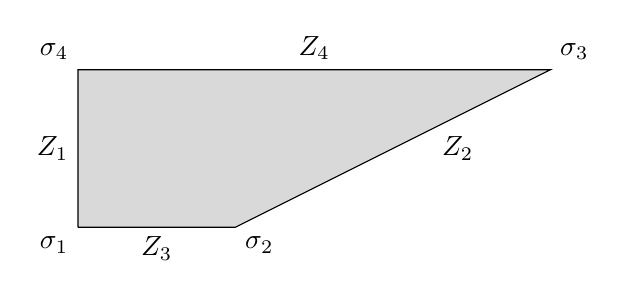
\begin{tikzpicture}
 \draw[fill=gray!30] (0,0)node[below left]{$\sigma_1$} --node[below]{$Z_3$} (2,0)node[below right]{$\sigma_2$} --node[right=.5cm]{$Z_2$} (6,2)node[above right]{$\sigma_3$} --node[above]{$Z_4$} (0,2)node[above left]{$\sigma_4$} --node[left]{$Z_1$} (0,0);
 \end{tikzpicture}
\end{center}
The cohomology ring is given by:
\[
 H^*(\mathbb F_2,\ZZ)\simeq\ZZ[Z_1,\ldots,Z_4]/\langle Z_1-Z_2,Z_4-Z_3-2Z_2, Z_1Z_2,Z_3Z_4\rangle
\]
We work out the following weights for the $\Gm^4$-action:

\begin{center}
 \begin{tabular}{||c|c||c|c||}
  \hline
  $\lambda^{\sigma_1}_{\sigma_2}=-\lambda^{\sigma_2}_{\sigma_1}$ & $\lambda_1-\lambda_2$ & $\lambda^{\sigma_3}_{\sigma_4}=-\lambda^{\sigma_4}_{\sigma_3}$ & $\lambda_2-\lambda_1$ \\
  \hline
  $\lambda^{\sigma_2}_{\sigma_3}=-\lambda^{\sigma_3}_{\sigma_2}$ & $2\lambda_1+\lambda_3-\lambda_4$ & $\lambda^{\sigma_4}_{\sigma_1}=-\lambda^{\sigma_1}_{\sigma_4}$ & $\lambda_4-2\lambda_2-\lambda_3$ \\
  \hline
 \end{tabular}
\end{center}

When thinking of them as curve classes, I shall write $F=[Z_1], D_0=[Z_4], D_\infty=[Z_3]$. I am going to compute $\langle Z_3,Z_4,Z_1Z_4\rangle^{\mathbb F_2,\epsilon}_{0,3,D_\infty+F}$ for $\epsilon=\infty,0+$.

The relevant graphs in the stable maps case are:
\begin{center}
 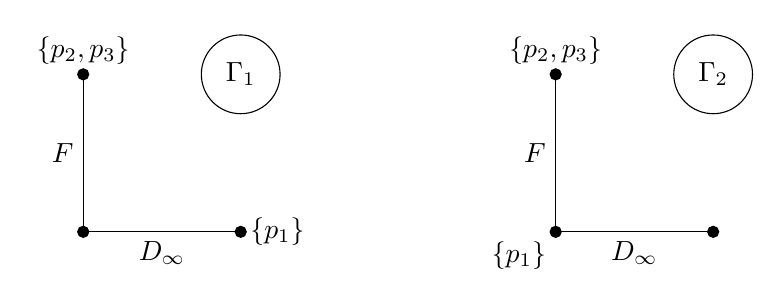
\begin{tikzpicture}[radius=2pt]
  \draw[fill=black] (0,2) circle node[above]{$\{p_2,p_3\}$};
  \draw[fill=black] (0,0) circle;
  \draw[fill=black] (2,0) circle node[right]{$\{p_1\}$};
  \draw (0,2) --node[left]{$F$} (0,0) -- node[below]{$D_\infty$} (2,0);
  \draw (2,2) circle (.5cm) node{$\Gamma_1$};
  %
  \draw[fill=black] (6,2) circle node[above]{$\{p_2,p_3\}$};
  \draw[fill=black] (6,0) circle node[below left]{$\{p_1\}$};
  \draw[fill=black] (8,0) circle;
  \draw (6,2) --node[left]{$F$} (6,0) -- node[below]{$D_\infty$} (8,0);
  \draw (8,2) circle (.5cm) node{$\Gamma_2$};
 \end{tikzpicture}
\end{center}
For $\epsilon=0+$, $\Gamma_2$ is unstable, and we have instead to consider:
\begin{center}
 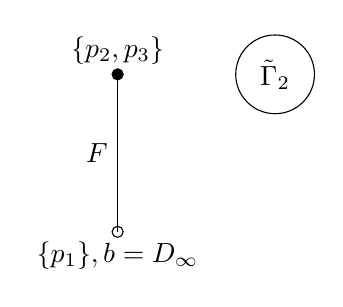
\begin{tikzpicture}[radius=2pt]
  \draw[fill=black] (0,2) circle node[above]{$\{p_2,p_3\}$};
  \draw[fill=white] (0,0) circle node[below]{$\{p_1\},b=D_\infty$};
  \draw (0,2) --node[left]{$F$} (0,0);
  \draw (2,2) circle (.5cm) node{$\tilde\Gamma_2$};
 \end{tikzpicture}
\end{center}
The white circle indicates a basepoint component. It can be verified that:
\[ \langle Z_3,Z_4,Z_1Z_4\rangle^{\mathbb F_2,\infty}_{0,3,D_\infty+F}=-1 \quad \text{while} \quad \langle Z_3,Z_4,Z_1Z_4\rangle^{\mathbb F_2,0+}_{0,3,D_\infty+F}=-2.\]



\section{Relative quasimaps}\label{sec:rel_qm}
The relative problem in Gromov-Witten theory consists in studying maps satisfying not only incidence conditions, but also a tangency requirement to a divisor. It has seen great advancements in the past twenty years, of which I will sample some most relevant ones in algebraic geometry (there is an almost parallel and similarly rich story in symplectic geometry):
\begin{itemize}
 \item R. Vakil's pioneering work on rational and elliptic curves in projective space, satisfying tangency conditions to a hyperplane \cite{Vre};
 \item A. Gathmnn's work in genus $0$, enhancing the previous one to the case of a smooth very ample divisor in any variety \cite{Ga};
 \item J. Li's moduli space of maps to expanded targets, removing the ampleness hypothesis on the divisor and developing the framework for the all important degeneration formula \cite{Li1,Li2}, which has been reviewed by B. Kim in a more explicitly logarithmic \cite{KimLog}, and by D. Abramovich and B. Fantechi in a more stacky \cite{AbramovichFantechi} context;
 \item a host of recent works around D. Abramovich, Q. Chen, M. Gross, and B. Siebert's space of logarithmic stable maps \cite{ChenLog,AbramovichChenLog,GrossSiebertLog}, which allows for example the divisor to be snc.
\end{itemize}
It would be interesting to have a full relative theory for $\epsilon$-quasimaps, including a degeneration formula and wall-crossing formulae for relative invariants as well; one application (suggested by I. Ciocan-Fontanine) would be to the study of the higher genus $\epsilon$-quasimap invariants of the quintic threefold via Maulik-Pandharipande's degeneration scheme \cite{MauPan}. In \cite{BN} we have made a first step towards this program, namely we have introduced spaces of genus $0$ relative quasimaps to a smooth very ample divisor, extending the work of Gathmann. Among the peculiarities of this approach are the fact that the tangency needs not be maximal (i.e. not all intersection points of the curve with the divisor must be marked with the respective tangency order requirement), and the fact that the relative spaces are nested (they become smaller as the tangency requirement gets higher), with a nice formula expressing their virtual classes in terms of one another, corrected by a boundary term exhibiting a clear recursive structure. This led Gathmann to the discovery of an algorithm for computing relative invariants, or, even further, restricted invariants of the hyperplane section, recursively, starting from the descendant theory of the ambient space; under positivity assumptions, he was able to realise this in a different proof of what goes under the name of Givental's mirror theorem, or the quantum Lefschetz principle \cite{Ga-MF}. In this section I will report on my work with N. Nabijou.
\subsection{Review of Gathmann's work} The starting point is the case of $\PP^N$ relative to a hyperplane $H$. The most down-to-earth approach works in this case: chosen a tangency condition $\alpha\in\N^n$ with $\sum\alpha\leq d$, Gathmann defines the relative space $\M{0}{\alpha}{\PP^N|H}{d}\subseteq \M{0}{n}{\PP^N}{d}$ as the closure of the ``nice'' locus of maps $f\colon(\PP^1,\mathbf x)\to \PP^N$ such that $f(\PP^1)\subsetneq H$ and $f^{-1}(H)-\sum\alpha_ix_i$ is an effective divisor. He then proves that the reducible maps that lie in the closure can be characterised combinatorially as follows:
 a stable map $(C,x_1, \ldots, x_n,f)$ is in $\M{0}{\alpha}{\PP^N|H}{d}$ if and only if, for each connected component $Z$ of $f^{-1}(H) \subseteq C$:
\begin{enumerate}
\item if $Z$ is a point and is equal to a marked point $x_i$, then $f$ is tangent to $H$ at $x_i$ to order $\alpha_i$ at least;
\item if $Z$ is a curve, and if we let $C^{(i)}$ for $1 \leq i \leq r$ denote the irreducible components of $C$ adjacent to $Z$, and $m^{(i)}$ denote the multiplicity of $f|_{C^{(i)}}$ to $H$ at the node $Z \cap C^{(i)}$, then:
\begin{equation} \label{Relative stable map internal component inequality} H \cdot f_* [Z] + \sum_{i=1}^r m^{(i)} \geq \sum_{x_i \in Z} \alpha_i \end{equation}
\end{enumerate}
Now this definition works well for every pair $(X|Y)$ of a variety with a smooth divisor, by just replacing $H$ with $Y$ in the description above. On the other hand, the definition as the closure of the nice locus makes it clear that $\M{0}{\alpha}{\PP^N|}{d}$ is irreducible of the expected dimension: \[\dim(\M{0}{\alpha}{\PP^N|H}{d})=\dim (\M{0}{n}{\PP^N}{d})-\sum\alpha.\]
If we then assume that $Y$ is very ample, we may use the complete linear system associated to it in order to embed $\phi_{\lvert Y\rvert}\colon X\hookrightarrow\PP^N$ and find a hyperplane $H\subseteq \PP^N$ such that $H\cap X= Y$. Set $d=\phi_{\lvert Y\rvert,*}(\beta)$ for a curve class $\beta\in H_2^+(X)$. The following cartesian diagram holds true:
\bcd
\M{0}{\alpha}{X|Y}{\beta}\ar[d]\ar[r]\ar[dr,phantom,"\Box"] & \M{0}{n}{X}{\beta}\ar[d,"\Phi_{\lvert Y\rvert}"] \\
\M{0}{\alpha}{\PP^N|H}{d} \ar[r] & \M{0}{n}{\PP^N}{d}
\ecd
Furthermore $\operatorname{R}^\bullet\pi_*f^*N_{X/\PP^N}$ provides a compatible perfect (by the unobstructedness of $\M{0}{n}{\PP^N}{d}$) obstruction theory for $\Phi_{\lvert Y\rvert}$, hence we may endow $\M{0}{\alpha}{X|Y}{\beta}$ with a virtual class
\[ \virt{\M{0}{\alpha}{X|Y}{\beta}}=\Phi_{\lvert Y\rvert}^![\M{0}{\alpha}{\PP^N|H}{d}] \]
which also has the expected codimension $\sum\alpha$ with respect to $\virt{\M{0}{n}{X}{\beta}}$.

As anticipated, the combinatorial description shows that $\M{0}{\alpha+e_k}{X|Y}{\beta}\subseteq \M{0}{\alpha}{X|Y}{\beta}$, and it is a divisor. Gathmann finds a natural line bundle with section that cuts it out, together with a number of boundary correction terms.

Let me start with some heuristic: assume $n=1$ for this. Let $Y=V(s)\subseteq X$. Then $\M{0}{(1)}{X|Y}{\beta}\subseteq \M{0}{1}{X}{\beta}$ is cut out by the section $\ev_1^*(s)$ of $\ev_1^*\OO_X(Y)$.

Now the restriction of $\ev_1$ to $\M{0}{(1)}{X|Y}{\beta}$ lands into $Y$; by composing $df_{x_1}\colon TC_{x_1}\to TX_{f(x_1)}$ with the projection to $N_{Y/X,f(x_1)}$ we get a map that has to vanish if $f$ is tangent to $H$ at $x_1$. Rearranging we get a section $\ev_1^*(d^1s)$ of $x_1^*(T^*C)\otimes\ev_1^*\OO_X(Y)$ that defines $\M{0}{(2)}{X|Y}{\beta}$ within $\M{0}{(1)}{X|Y}{\beta}$.

More generally we may use the jet bundles (or bundles of principal parts) of $\OO_X(Y)$: there is an exact sequence
\[ 0\to x_1^*\Omega_{C}^{\otimes m+1}\otimes\ev_1^*\OO_X(Y)\to ev_1^*\mathcal P^{m+1}(\OO_X(Y))\to ev_1^*\mathcal P^{m}(\OO_X(Y))\to 0\]
and $s$ induces a section $\ev_1^*(d^{m+1}s)$ of the middle term (which should be thought of as the Taylor expansion of $s$ at $x_1$ up to order $m+1$), the image of which in the rightmost term (i.e. its truncation up to order $m$) vanishes on $\M{0}{(m)}{X|Y}{\beta}$, hence inducing a section of the line bundle $x_1^*\Omega_{C}^{\otimes m+1}\otimes\ev_1^*\OO_X(Y)$ which vanishes along $\M{0}{(m+1)}{X|Y}{\beta}$. Notice though that it also vanishes (for every $m$, really) on those maps such that the irreducible component containing $x_1$ is mapped entirely into $Y$. We have thus arrived to Gathmann's formula:
\begin{thm}\cite[Theorem 2.6]{Ga}\label{thm:Gathmann_formula} In the Chow group of $\M{0}{\alpha}{X|Y}{\beta}$
 \begin{equation*} (\alpha_k \psi_k + \ev_k^* \OO_X(Y)) \cap \virt{\M{0}{\alpha}{X|Y}{\beta}} = \virt{\M{0}{\alpha+e_k}{X|Y}{\beta}} + \virt{\mathcal{D}_{\alpha,k}(X,\beta)} \end{equation*}
\end{thm}
where $\mathcal{D}_{\alpha,k}(X,\beta)$ is a sum over all
\begin{itemize}
 \item $r\geq 0$ determining the number of adjacent external components $C^{(1)},\ldots,C^{(r)}$,
 \item $M=(m^{(1)},\ldots,m^{(r)})\in \N^r_{>0}$ determining the order of contact of $C^{(i)}$ with $Y$ at the intersection with the internal component $C^{(0)}$,
 \item $A=(\alpha^{(0)},\ldots,\alpha^{(r)})$ and $B=(\beta_0,\ldots,\beta_r)$ dictating the splitting of the markings/tangency requirements and curve class respectively,
\end{itemize}
   of the following ``comb loci'':
\[\mathcal{D}_{A,B,M}(X)=\M{0}{\lvert\alpha^{(0)}\rvert+r}{Y}{\beta_0}\times_{H^r}\prod_{i=1}^r
\M{0}{\alpha^{(i)}\cup m^{(i)}}{X|Y}{\beta_i}\]
These are endowed with the product virtual fundamental class, weighted by a factor $\frac{m^{(1)}\cdot\ldots\cdot m^{(r)}}{r!}$; the denominator is just there to make the auxiliary gluing markings unordered, while in a sense the numerator is the real content of Gathmann's formula. As noticed above the section $\ev_k^*(d^ms)$ vanishes whenever $x_k$ lies on an internal component; the sum must therefore run over all those splitting types such that $\mathcal{D}_{A,B,M}(X)$ lies in $\M{0}{\alpha}{X|Y}{\beta}$ but not in $\M{0}{\alpha+e_k}{X|Y}{\beta}$, namely those satisfying $\alpha_k\in\alpha^{(0)}$ and
\[\OO_X(Y)\cdot\beta_0+\sum M=\sum \alpha^{(0)}.\]
The proof goes roughly as follows: the reduction to the case of $(\PP^N|H)$ is just a matter of virtual intersection calculus; in the unobstructed case the shape of the formula follows simply from the above arguments and a(n actual) dimension computation, so the hard part is to get the coefficients right. Locally one may reduce further to $(\PP^1,\{\infty\})$ by projecting from a generic $(N-2)$-plane inside $H$; finally the proof for $\PP^1$ is based on Vakil's observation that, for maps from cuves to curves, the obstruction theory only sees the special loci (markings, nodes, ramification points, and contracted components), so that one can split the deformation space and reduce to a much simpler moduli problem.
\begin{rmk}\label{rmk:expandedGathmann}
 Gathmann's recursion can be recovered in the framework of Jun Li's spaces of maps to expansions (or rather Kim's logarithmic stable maps). This was suggested by J. Wise and D. Ranganathan. It may seem surprising but in fact the idea of reducing from non-maximal to maximal tangency order was already contained in the proof of Gathmann's formula. Here is the strategy to get Theorem \ref{thm:Gathmann_formula} for $(\PP^N|H)$ using maps to expansions: add $h=d-\sum\alpha$ auxiliary markings of multiplicity $1$, so consider $\MK{0}{\alpha\cup(1,\ldots,1)}{\PP^N|H}{d}$. Call $c_h$ the map forgetting the auxiliary markings and the log structures, collapsing the target, and stabilising the source curve, which is an $(h!:1)$ cover of $\M{0}{\alpha}{\PP^N|H}{d}$ (generically we are just marking the $h$ simple unmarked intersections of the image of $C$ with $H$, and endowing $C$ with the pullback of the divisorial log structure on $\PP^N$; here we use that $g=0$ and the target is $\PP^N$, but notice that the approach will work whenever the nice locus is dense in the relative space). Denote instead by $c\colon \MK{0}{\alpha\cup(1,\ldots,1)}{\PP^N|H}{d}\to \M{0}{\alpha\cup(1,\ldots,1)}{\PP^N}{d}$ the map that forgets the log structures, collapses the target, and stabilises the source curve; we may then pullback Gathmann's line bundle and section along $c$. The vanishing locus of the section thus obtained consists of maps such that the target is expanded, and $x_k$ lies on a non-trivial (i.e. having either positive horizontal degree, or at least three markings) component at higher level. Notice that, as soon as there is more than one non-trivial component at higher level, $c$ has positive-dimensional fibers. Hence we are reduced to a sum over bipartite graphs with only one vertex at higher level; we recognise in these the shape of the comb loci appearing in Gathmann's formula. Also, I claim that the only term that survives pushforward under $c_h$, and in which one of the auxiliary markings (say $x_{n+1}$) may lie on the component containing $x_k$, is when the latter has zero horizontal degree and contains only $x_k$ and $x_{n+1}$ among the markings - otherwise the map collapsing the target and forgetting the auxiliary markings will have positive dimensional fibers. This recovers $\M{0}{\alpha+e_k}{\PP^N|H}{d}$. 
 \begin{center}
 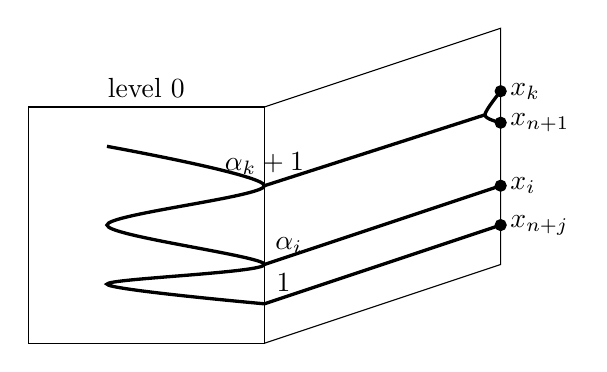
\begin{tikzpicture}
 \draw (0,0) -- (3,0) -- (3,3) -- node[above]{level $0$} (0,3) -- (0,0);
 \draw (3,0) -- (6,1) -- (6,4) -- (3,3);
 \draw[very thick] plot [smooth] coordinates {(1,2.5) (3,2) (1,1.5) (3,1) (1,0.75) (3,.5)};
 \draw[very thick] (3,2) node[above]{$\alpha_k+1$} -- (5.8,2.9) (3,1) node[above right]{$\alpha_i$} -- (6,2) (3,.5) node[above right=.5]{$1$} -- (6,1.5);
 \draw[very thick] plot [smooth] coordinates {(6,3.2) (5.8,2.9) (6,2.8)};
 \draw[black,fill=black] (6,3.2) circle[radius=2pt] node[right]{$x_k$} (6,2.8) circle[radius=2pt] node[right]{$x_{n+1}$} (6,2) circle[radius=2pt] node[right]{$x_i$} (6,1.5) circle[radius=2pt] node[right]{$x_{n+j}$};
\end{tikzpicture}
\end{center}
 
 The claim follows from the fact that the rubber space $\M{0}{\mu}{\PP_H(\OO\oplus\OO(1))}{\beta_0}^\thicksim$ has the same dimension as $\M{0}{\lvert\mu\rvert}{H}{\beta_0}$, see \cite[\S 2.4]{GraberVakil}. Now the coefficient with which each of these loci appears has been computed by several authors in the framework of the degeneration formula (see e.g. \cite[Remark 6.3.1.2]{KimLog} and \cite[Equation (1.7)]{KLR}):  the log structure is determined at the level of ghost sheaves by the underlying morphism, and the numerator counts the number of log liftings, while the denominator again clears out the ordering of the edges. There is one more subtelty, as noticed by Gathmann already \cite[Corollary 3.5]{Ga}: $\M{0}{\alpha+e_k}{\PP^N|H}{d}$ appears on one side with a coefficient $\alpha_k+1$, which is partially cancelled by an $\alpha_k$ on the other side, arising from the comparison between $\psi_k$ and $\fgt_{n+1,\ldots,n+h}^*\psi_k$. All the degeneracy loci that persist under $c_h$-pushforward cover $(h!:1)$ one of the comb loci in Gathmann's formula.
\end{rmk}

\subsection{Definitions and propositions}
I come now to the definition of relative quasimaps \cite[\S 2.3]{BN}. Let $X$ be a smooth toric variety, $Y=V(s)$ a smooth very ample divisor (not necessarily toric). As in the discussion of functoriality (Section \ref{sec:functoriality}), we may write $\OO_X(Y)=\bigotimes_{\rho\in\Sigma(1)}\OO_X(D_\rho)^{\otimes a_\rho}$ and 
\[s=\sum_{\mathbf a:[\mathbf a]=\OO_X(Y)}\mu_{\mathbf a}\prod_{\rho\in\Sigma(1)}z_\rho^{a_\rho}\]
in terms of Cox's homogeneous coordinates. For a quasimap 
\[ \Big((C,x_1,\ldots,x_n), (L_\rho,u_\rho)_{\rho \in \Sigma(1)}, (\varphi_m)_{m \in M}\Big) \]
set $L_Y=\bigotimes_{\rho\in\Sigma(1)}L_\rho^{\otimes a_\rho}$ and
\[u_s=\mu_{\mathbf a}\prod_{\rho\in\Sigma(1)}u_\rho^{a_\rho}+\sum_{\mathbf a\neq \mathbf b:[\mathbf b]=\OO_X(Y)}\mu_{\mathbf b}\varphi_{\mathbf b-\mathbf a}\left(\prod_{\rho\in\Sigma(1)}u_\rho^{b_\rho}\right)\in H^0(C,L_Y).\]
%\appendix
\begin{definition}
 A quasimap belongs to \emph{the relative space} $\Q{0}{\alpha}{X|Y}{\beta}\subseteq \Q{0}{n}{X}{\beta}$ if for every connected component $Z$ of $u_s^{-1}(0)$, the following holds:
\begin{enumerate}
\item if $Z$ is a point and is equal to a marking $x_i$, then $u_s^*(0)$ has order at least $\alpha_i$ at $x_i$;
\item if $Z$ is a curve, and if we let $C^{(i)}$ for $1 \leq i \leq r$ denote the irreducible components of $C$ adjacent to $Z$, and $m^{(i)}$ denote the multiplicity of $f|_{C^{(i)}}$ to $H$ at the node $Z \cap C^{(i)}$, then:
\begin{equation} \label{Relative quasimap internal component inequality} \deg(L_{Y}|_Z) + \sum_{i=1}^r m^{(i)} \geq \sum_{x_i \in Z} \alpha_i \end{equation}
\end{enumerate}
\end{definition}

I am going to discuss an adaptation of Gathmann's recursion formula to this setup: the idea is to push down Theorem \ref{thm:Gathmann_formula} along the collapsing morphism (Section \ref{sec:collapsing}) in the case of $(\PP^N|H)$, and then recover the general formula by virtual pullback.

\begin{lem}
 The collapsing morphism $\chi$ restricts to a proper and birational morphism \[\chi_\alpha\colon \M{0}{\alpha}{\PP^N|H}{d}\to \Q{0}{\alpha}{\PP^N|H}{d}.\]
\end{lem}
\begin{proof}
 We first show that a stable map satisfying \eqref{Relative stable map internal component inequality} is sent to a quasimap satisfying \eqref{Relative quasimap internal component inequality}: the collapsing of rational tails happens far from any markings, so we only have to discuss the case of an internal component $Z$. If the rational tail $R$ is internal, then collapsing does not affect the left hand side of the inequality (it simply transfers some degree from $R$ to $\overline{Z\setminus R}$); on the other hand, if it is external, collapsing may only increase the left hand side, since the multiplicity of contact $m^R$ is at most equal to the degree of $f_{|R}$. This proves that $\chi(\M{0}{\alpha}{\PP^N|H}{d})\subseteq \Q{0}{\alpha}{\PP^N|H}{d}$.
 
 On the other hand $\chi_\alpha$ is surjective: given a relative quasimap $\xi'$ with an internal basepoint $q_0$ of order $d_0$, choose any line $\ell$ through its image, with $\ell$ transverse to $H$, and lift $\xi'$ to a stable map $\xi$ by adjoining a $\PP^1=:R$ to the source curve at $q_0$, and defining the map $f_{|R}$ to be a $d_0$-fold cover of $\ell$ totally ramified at $q_0$ (any basepoint which is not internal is easier to deal with).
 
 Now, given any relative quasimap $\xi'\in\Q{0}{\alpha}{\PP^N|H}{d}$ we may choose a lifting $\xi\in\M{0}{\alpha}{\PP^N|H}{d}$; by Gathmann's result, $\xi$ can be smoothed to a map in the nice locus; applying $\chi$ to such a smoothing we obtain a smoothing of $\xi'$. This shows that $\Q{0}{\alpha}{\PP^N|H}{d}$ is contained in the closure of the nice locus of relative quasimaps with no basepoints and image not contained in $H$. On the other hand $\Q{0}{\alpha}{\PP^N|H}{d}$ is closed by the principle of conservation of number. Therefore $\chi_\alpha$ is proper and birational, being an isomorphism on the nice locus.
\end{proof}

\begin{prop}\label{prop:quasimap_Gathmann_formula} In the Chow group of $\Q{0}{\alpha}{X|Y}{\beta}$
 \begin{equation*} (\alpha_k \psi_k + x_k^*c_1(L_Y)) \cap \virt{\Q{0}{\alpha}{X|Y}{\beta}} = \virt{\Q{0}{\alpha+e_k}{X|Y}{\beta}} + \virt{\mathcal{D}^Q_{\alpha,k}(X,\beta)} \end{equation*}
\end{prop}
\noindent where $\mathcal{D}^Q_{\alpha,k}(X,\beta)$ is a sum of ``comb loci'', running over all splittings $A,B,M$ of the markings, curve class, and multiplicities at the internal-to-external nodes, this time required to satisfy the quasimap stability condition (in particular there are no rational tails):
\[\mathcal{D}^Q_{A,B,M}(X)=\Q{0}{\lvert\alpha^{(0)}\rvert+r}{Y}{\beta_0}\times_{H^r}\prod_{i=1}^r
\Q{0}{\alpha^{(i)}\cup m^{(i)}}{X|Y}{\beta_i}\]
endowed with the product virtual fundamental class, weighted by a factor $\frac{m^{(1)}\cdot\ldots\cdot m^{(r)}}{r!}$.
\begin{proof}
 In the case of $(\PP^N|H)$ the result follows by pushing forward Gathmann's formula along $\chi_\alpha$: for this it is useful to notice that
 \begin{equation}
  \chi^*(\psi_k)=\psi_k, \quad \text{and} \quad \chi^*(x_k^*L_Y)=\ev_k^*\OO_X(Y),
 \end{equation}
because collapsing does not affect the universal curve in a neighbourhood of the marking $x_k$. On the other hand if a comb locus $\mathcal{D}^Q_{A,B,M}(X)$ contains a rational tail (necessarily external), then the restriction of $\chi$ to $\mathcal{D}^Q_{A,B,M}(X)$ has positive dimensional fibers, because $\dim(\M{0}{(m^{(i)})}{\PP^N|H}{d})>\dim H$, so the corresponding term of Gathmann's formula vanishes under $\chi_*$.

The case of a smooth very ample divisor $(X|Y)$ follows by virtual pullback: $\Q{0}{n}{\PP^N}{d}$ is unobstructed, hence the  closed embedding $\phi_{\lvert Y\rvert}\colon X\hookrightarrow \PP^N$ induces $\Phi_{\lvert Y\rvert}\colon \Q{0}{n}{X}{\beta}\to \Q{0}{n}{\PP^N}{d}$ endowed with a perfect obstruction theory.

$\Phi_{\lvert Y\rvert}^![\Q{0}{\alpha}{\PP^N|H}{d}]=\virt{\Q{0}{\alpha}{X|Y}{\beta}}$ by the very definition of the latter, and it is easily checked that $\Phi_{\lvert Y\rvert}^![\Q{0}{a_0+r}{H}{d_0}]=\virt{\Q{0}{a_0+r}{Y}{\beta_0}}$ where the latter is defined as in \cite{CFKM}. The fact that the fundamental class of a comb locus pulls back to the corresponding virtual class follows from the splitting property of the virtual class of quasimap spaces (Section \ref{sec:cohFT}); this has been checked in all details in \cite[\S 4 and Appendix B.4]{BN}.
\end{proof}

\subsection{Gathmann's algorithm and quasimap quantum Lefschetz} Notice that in the very last step of the recursion, i.e. increasing $\sum\alpha$ from $Y\cdot \beta$ to $Y\cdot \beta+1$, there is no main term but only boundary corrections; also, for one of them there are no external components, which recovers $\Q{0}{n}{Y}{\beta}$.

Gathmann describes an algorithm for computing relative invariants of $(X|Y)$ and \ilemph{restricted} absolute invariants of $Y$ (i.e. the cohomological insertions lie in the image of the restriction map $i^*\colon H^*(X)\to H^*(Y)$) recursively, assuming that we know the descendant invariants of $X$. The proof is by induction on the numerical invariants (i) $d=Y\cdot \beta,$ (ii) $n,$ and (iii) $\sum\alpha$ (convention: for absolute invariants of $Y$ set $\sum\alpha=d+1$). If we want to compute a relative invariant with tangency condition $\alpha$ and degree $\beta$, assume $\alpha_k>0$ (if we cannot find such a $k$ then we are just considering an absolute invariant of $X$); we may then write down the formula as
\[\virt{\Q{0}{\alpha}{X}{\beta}}=((\alpha_k-1)\psi_k+\ev_k^*\OO_X(Y))\virt{\Q{0}{\alpha-e_k}{X}{\beta}}-\virt{\mathcal{D}^Q_{\alpha-e_k,k}(X,\beta)}\]
The classes appearing on the right hand side have lower numerical invariants, so we may assume they have been computed inductively. There is a delicate point, namely that we use the cohomological splitting of the diagonal of $Y\times Y$ in order to reduce the integrals on comb loci to products of relative $(X|Y)$ and absolute $Y$ invariants, but in doing so we might introduce some non-restricted insertions.

It can be proved that invariants of $Y$ comprising only one unrestricted insertion vanish: assume we are interested in $\langle\tau_{a_1}(\delta_1),\ldots,\tau_{a_n}(\delta_n)\rangle^{Y,0+}_{0,n,\beta}$ with only $\delta_1\in i^*H^*(X)^\perp$. Recall that $i_*\virt{\Q{0}{n}{Y}{\beta}}=c_{\text{top}}(\pi_*f^*\OO_X(Y))\cap \virt{\Q{0}{n}{X}{i_*\beta}}$ follows from pulling back the analogous statement for $(\PP^N|H)$, and we may write $c_{\text{top}}(\pi_*f^*\OO_X(Y))=\ev_1^*\OO_X(Y)c_{\text{top}}(E^{Y\cdot\beta})$ for a certain vector bundle $E^{Y\cdot\beta}$. Consider the following factorisation:
\bcd
\Q{0}{(1,0,\ldots,0)}{X|Y}{\beta}\ar[r,"j"]\ar[d,"\tilde\ev_1"] & \Q{0}{n}{X}{\beta}\ar[d,"\ev_1"] \\
Y\ar[r,"i"] & X
\ecd
and $\langle\tau_{a_1}(\delta_1),\ldots,\tau_{a_n}(\delta_n)\rangle^{\epsilon,Y}_{0,n\beta}$ is computed by
\begin{multline*}
 \delta_1\cdot\tilde\ev_{1,*}i^!\left(\psi_1^{a_1}\prod_{i=2}^n\ev_i^*(\delta_i)\psi_i^{a_i}c_{\text{top}}(E^{Y\cdot\beta})\cap\virt{\Q{0}{n}{X}{\beta}}\right)= \\
 \delta_1\cdot i^*\ev_{1,*}\left(\psi_1^{a_1}\prod_{i=2}^n\ev_i^*(\delta_i)\psi_i^{a_i}c_{\text{top}}(E^{Y\cdot\beta})\cap\virt{\Q{0}{n}{X}{\beta}}\right) =0
\end{multline*}
It is then possible to prove recursively that any relative invariant with only one unrestricted invariant vanishes (see \cite[Lemma 5.6]{Ga}), and this is sufficient for our application, since the external components always get at most one such insertion.

\smallskip

Under some positivity assumptions - which allow us to discard most contributions from the comb loci by dimensional reasons -, the algorithm above can be realised into a compact formula, relating some astutely chosen combination of quasimap invariants of $Y$ to those of $X$ . The following discussion (from \cite[\S 5]{BN}) is inspired by \cite{Ga-MF}, in which Gathmann applies the stable map recursion formula to obtain a new proof of the mirror theorem for hypersurfaces \cite{Givental-equivariantGW}.

From now on we make the following two assumptions:
\begin{enumerate}
\item \emph{$Y$ is semi-positive}: $-K_Y$ is nef;
\item \emph{$Y$ contains all curve classes}: the map $i_* : \Achow_1(Y) \to \Achow_1(X)$ is surjective.
\end{enumerate}
\begin{rmk}
 By adjunction, $-K_X$ pairs strictly positively with every curve class coming from $Y$, hence with every curve class by Assumption (2). Thus $-K_X$ is ample, or in other words $X$ is Fano, by Kleiman's criterion, since the effective cone of the toric variety $X$ is finitely generated in $\Achow_1(X)$, hence is closed in $\Achow_1(X)_{\mathbb{R}}$. Also note that if $\dim X \geq 3$ Assumption (2) always holds, due to the classical Lefschetz hyperplane theorem; on the other hand if $\dim X = 2$ Assumption (2) forces $X$ to be $\PP^2$.
\end{rmk}

Recall that we have fixed a homogeneous basis $\eta_0, \ldots, \eta_l$ for $\HH^*(X) = \HH^*(X,\QQ)$ and let $\eta^0, \ldots, \eta^l$ denote the dual basis with respect to the Poincar\'e pairing. Without loss of generality we may suppose that $\eta^0=\mathbbm 1_X$ and $\eta^1=[Y]$. We get an induced basis $\rho_1=i^*\eta_1, \ldots, \rho_l = i^* \eta_l$ for $i^*\HH^*(X)$. Notice that $\rho_0 = i^* \eta_0 = i^* [\pt_X] = 0$, $\rho_1 = i^* \eta_1 = [\pt_Y]$.  We can extend the $\rho_i$ to a basis $\rho_1, \ldots, \rho_k$ for $\HH^*(Y)$ by adding $\rho_{l+1}\ldots,\rho_{k}$. Let $\rho^1, \ldots, \rho^k$ denote the dual basis; notice that $\rho^i$ is \emph{not} equal to $i^* \eta^i$, and $\rho^1 = \mathbbm{1}_Y$.

We are going to analyse the behaviour of a generating function of $2$-pointed quasimap invariants with a fundamental class insertion, which in fact coincides with the small $I$-function from Section \ref{subsec:gf_and_wc}. Let me break the notation into two: for any smooth projective toric variety $X$ and any effective curve class $\beta\in \HH_2^+(X)$, define
\begin{align*} S_0^X(z,\beta) & =(\ev_1)_*\left(\frac{1}{z-\psi_1} \virt{\Q{0}{2}{X}{\beta}}\right) 
\intertext{and then the small $I$-function is}
S_0^X(z,q) &=\sum_{\beta\geq 0} q^\beta S_0^X(z,\beta)\end{align*}
where by convention $S_0^X(z,0)= \mathbbm 1_X$; this function takes values in $\HH^*(X,\Lambda)$ and the notation is reminiscent of $I(q,z)=S^{0+}(q,0,z)(\mathds 1)$.

The same definition applies to $Y$. However we may wish to consider only restricted insertions, and we therefore set
\begin{equation*} \tilde{S}^Y_0(z,\beta) = (\ev_1)_* \left( \dfrac{1}{z-\psi_1} \virt{\Q{0}{2}{Y}{\beta}} \right) \end{equation*}
where crucially $\ev_1$ is viewed as mapping to $X$ instead of to $Y$. Remark that $i_* S^Y_0(z,\beta) = \tilde{S}^Y_0(z,\beta)$ (since $X$ and $Y$ are smooth, we may use Poincar\'{e} duality to define a push-forward map on cohomology, $i_* \colon \HH^k(Y) \to \HH^{k+2}(X)$).

\begin{thm} \label{Theorem Quantum Lefschetz}
Let $X$ and $Y$ be as above. Then
\begin{equation}\label{eqn:mirror}
\dfrac{\sum_{\beta\geq 0} q^\beta\prod_{j=0}^{Y\cdot\beta}(Y+jz)S_0^X(z,\beta)}{P_0^X(q)}= \tilde{S}_0^Y(z,q)
\end{equation}
where:
\begin{align*}
 P_0^X(q) % & = 1 + \sum_{\substack{\beta>0 \\ K_Y\cdot\beta=0}} q^\beta (Y\cdot\beta) \langle [\pt_Y],\mathbbm 1_{X}\rangle_{0,(Y\cdot\beta,0),\beta}^{X|Y} \\
            & = 1 + \sum_{\substack{\beta>0 \\ K_Y\cdot\beta=0}} q^\beta(Y\cdot\beta)!\langle [\pt_X] \psi_1^{Y\cdot\beta-1} ,\mathbbm 1_{X}\rangle_{0,2,\beta}^X
\end{align*}
Notice that $P_0^X(q)$ depends not only on $X$ but also on the divisor class of $Y$ in~$X$; the superscript is supposed to indicate that the definition only involves quasimap invariants of $X$.
\end{thm}

\begin{proof}
For $m = 0, \ldots, Y \cdot \beta$, define the following generating function for $2$-pointed \emph{relative} quasimap invariants
 \[
  S_{0,(m)}^{X|Y}(z,\beta)=(\ev_1)_*\left(\frac{1}{z-\psi_1}\virt{\Q{0}{(m,0)}{X|Y}{\beta}}\right)
 \]
where we view $\ev_1$ as mapping to $X$.  Note that  $S_{0,(0)}^{X|Y}(z,\beta) = S_0^X(z, \beta)$. Also define the following generating function for ``comb loci invariants''
\[
 T_{0,(m)}^{X|Y}(z,\beta)=(\ev_1)_*\left(m \virt{\Q{0}{(m,0)}{X|Y}{\beta}}+\frac{1}{z-\psi_1} \virt{\mathcal{D}^{\mathcal{Q}}_{(m,0),1}(X|Y,\beta)} \right)
\]
where again we view $\ev_1$ as mapping to $X$. As in \cite[Lemma 1.2]{Ga-MF}, it follows from Proposition \ref{prop:quasimap_Gathmann_formula} that
\begin{equation}
 (Y+mz) S_{0,(m)}^{X|Y}(z,\beta) = S_{0,(m+1)}^{X|Y}(z,\beta)+ T_{0,(m)}^{X|Y}(z,\beta)
\end{equation}
and we can apply this repeatedly to obtain:
\begin{equation} \label{eqn:G}
\prod_{j=0}^{Y\cdot\beta}(Y+jz) S_0^X(z,\beta) = \sum_{m=0}^{Y\cdot\beta}\prod_{j=m+1}^{Y\cdot\beta}(Y+jz)T_{0,(m)}^{X|Y}(z,\beta)
\end{equation}
We now examine the right-hand side in detail. By definition, $T_{0,(m)}^{X|Y}(z,\beta)$ splits into two parts: those terms coming from the relative space and those terms coming from the comb loci.

Let us first consider the contribution of the comb loci. Since there are only two marked points and the first is required to lie on the internal component of the comb, it follows from the strong stability condition that there are only two options: a comb with zero teeth or a comb with one tooth.

First consider the case of a comb with zero teeth. The moduli space is then $\Q{0}{2}{Y}{\beta}$ and we require that $Y \cdot \beta = m$. Thus this piece only contributes to $T_{0,(Y\cdot\beta)}^{X|Y}(z,\beta)$, and the contribution is:
\begin{equation*} \sum_{i=1}^l \left\langle \dfrac{\rho_i}{z-\psi_1}, \mathbbm{1}_Y \right\rangle_{0,2,\beta}^Y \eta^i \end{equation*}

Next consider the case of a comb with one tooth. Let $\beta^{(0)}$ and $\beta^{(1)}$ denote the curve classes of the internal and external components, respectively, and let $m^{(1)}$ be the contact order of the external component with $Y$. The picture is as follows
\begin{center}
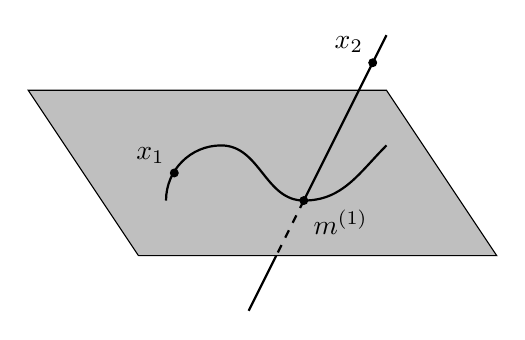
\begin{tikzpicture}[scale=0.7]
  \draw [fill=gray!50] (-.5,-1) -- (6,-1) -- (4,2) -- (-2.5,2) -- (-.5,-1);
  \draw [thick] (0,0) to [out=90,in=180] (1,1) to [out=0,in=180] (2.5,0) to [out=0,in=-135] (4,1);
  \draw [thick] (2.5,0) to (4,3);
  \draw [thick,dashed] (2.5,0) to (2,-1);
  \draw [thick] (2,-1) -- (1.5,-2);
  \draw [fill] (3.75,2.5) circle [radius=2pt] node[above left]{$x_2$};
  \draw [fill] (.15,.5) circle [radius=2pt] node[above left]{$x_1$};
  \draw [fill] (2.5,0.0) circle [radius=2pt] node[below right]{$m^{(1)}$};
 \end{tikzpicture}
\end{center}
and the invariants which contribute take the form
\begin{equation*} \bigg\langle \dfrac{\rho_i}{z-\psi_1},\rho^h\bigg\rangle_{0,2,\beta^{(0)}}^Y \bigg\langle \rho_h, \mathbbm 1_{X}\bigg\rangle_{0,(m^{(1)},0),\beta^{(1)}}^{X|Y} \end{equation*}
for $i = 1, \ldots, l$ and $h = 1, \ldots, k$. By computing dimensions, we find
\begin{align*}
0\leq \codim \rho^h &= \dim Y-\codim \rho_h \\
&= \dim Y-\vdim \Q{0}{(m^{(1)},0)}{X|Y}{\beta^{(1)}} \\
&= \dim Y-(\dim X-3-K_{X}\cdot \beta^{(1)}+2-m^{(1)})\\
&= K_Y \cdot \beta^{(1)} - Y \cdot \beta^{(1)}+m^{(1)} \\
&\leq 0
\end{align*}
where the final equality follows from adjunction and the final inequality holds because $-K_Y$ is nef and $m^{(1)}\leq Y \cdot \beta_1$. This shows that the only non-trivial contributions come from curve classes $\beta^{(1)}$ such that $K_Y \cdot \beta^{(1)}=0$, and that in this case the order of tangency must be maximal, i.e. $m^{(1)}=Y \cdot \beta^{(1)}$. Furthermore we must have $\codim \rho^h = 0$ and so $\rho^h = \rho^1 = \mathbbm{1}_Y$ which implies $\rho_h = \rho_1 = [\pt_Y]$. Finally since $m^{(1)}=Y \cdot \beta^{(1)}$ we have
\begin{equation*} m = Y \cdot \beta^{(0)}+m^{(1)}=Y \cdot (\beta^{(0)} + \beta^{(1)}) = Y \cdot \beta \end{equation*}
and so again this piece only contributes to $T_{0,(Y\cdot\beta)}^{X|Y}(z,\beta)$, and the contribution is:
\begin{equation*} \sum_{i=1}^l \left( \sum_{\substack{0 < \beta^{(1)} < \beta \\ K_Y \cdot \beta^{(1)}=0}} (Y \cdot \beta^{(1)}) \bigg\langle \dfrac{\rho_i}{z-\psi_1}, \mathbbm{1}_Y \bigg\rangle_{0,2,\beta-\beta^{(1)}}^Y \bigg\langle \rho_1, \mathbbm{1}_X \bigg\rangle_{0,(Y \cdot \beta^{(1)},0),\beta^{(1)}}^{X|Y} \right) \eta^i \end{equation*}
where the $Y \cdot \beta^{(1)}$ factor comes from the weighting on the virtual class of the comb locus. Finally, we must examine the terms of $T_{0,(m)}^{X|Y}(z,\beta)$ coming from:
\begin{equation*}\ev_{1*}(m\virt{\Q{0}{(m,0)}{X|Y}{\beta}})\end{equation*} 
Notice that we only have insertions from $i^*\HH^*(X) \subseteq \HH^*(Y)$, since $\ev_1$ is viewed as mapping to $X$. On the other hand
\begin{align*} \vdim \Q{0}{(m,0)}{X|Y}{\beta} & = \dim X-3 -K_X \cdot \beta +2-m & \\
& = \dim X - 1 -K_Y \cdot \beta + Y \cdot \beta - m \ \ & \text{by adjunction} \\
& \geq \dim X - 1 + Y\cdot\beta - m \ \ & \text{since $-K_Y$ is nef} \\
& \geq \dim X - 1 \ \ & \text{since $m \leq Y \cdot \beta$} \end{align*}
where in the second line we have applied the projection formula to $i$, and thus we have implicitly used Assumption (2), namely that every curve class on $X$ comes from a class on $Y$.

Consequently the only insertions that can appear are those of dimension $0$ and $1$. However, the restriction of the $0$-dimensional class $\eta_0 = [\pt_X]$ to $Y$ vanishes, as do the restrictions of all $1$-dimensional classes except for $\eta_1$ (by the definition of the dual basis, since $\eta^1 = Y$). Thus the only insertion is $i^*\eta_1=\rho_1=[\pt_Y]$, and since $\eta^1$ has dimension $1$ all the inequalities above must actually be equalities. Thus we only have a contribution if $-K_Y \cdot \beta = 0$ and $m = Y \cdot \beta$. The contribution to $T_{0,(Y\cdot\beta)}^{X|Y}(z,\beta)$ in this case is:
\begin{equation*} (Y \cdot \beta) \langle \rho_1 , \mathbbm{1}_X \rangle_{0,(Y \cdot \beta,0),\beta}^{X|Y} \eta^1 \end{equation*}

Thus we have calculated $T_{0,(m)}^{X|Y}(z,\beta)$ for all $m$; substituting into equation \eqref{eqn:G} we obtain
\begin{align*} \prod_{j=0}^{Y \cdot \beta} (Y + jz) & S_0^X(z,\beta) = T_{0,(Y\cdot\beta)}^{X|Y}(z,\beta) \\
= \ & \sum_{i=1}^l \left\langle \dfrac{\rho_i}{z-\psi_1}, \mathbbm{1}_Y \right\rangle_{0,2,\beta}^Y \eta^i + \\
& \sum_{i=1}^l \left( \sum_{\substack{0 < \beta^{(1)} < \beta \\ K_Y \cdot \beta^{(1)}=0}} (Y \cdot \beta^{(1)}) \bigg\langle \dfrac{\rho_i}{z-\psi_1}, \mathbbm{1}_Y \bigg\rangle_{0,2,\beta-\beta^{(1)}}^Y \bigg\langle \rho_1, \mathbbm{1}_X \bigg\rangle_{0,(Y \cdot \beta^{(1)},0),\beta^{(1)}}^{X|Y} \right) \eta^i + \\
& (Y \cdot \beta) \langle \rho_1 , \mathbbm{1}_X \rangle_{0,(Y \cdot \beta,0),\beta}^{X|Y} \eta^1
\end{align*}
where the third term only appears if $K_Y \cdot \beta=0$. We can rewrite this as:
\begin{align*} \prod_{j=0}^{Y \cdot \beta} (Y + jz) & S_0^X(z,\beta) \\
& = \tilde{S}_0^Y(z,\beta) + \sum_{\substack{0 < \beta^{(1)} \leq \beta \\ K_Y \cdot \beta^{(1)}=0}} \left( (Y \cdot \beta^{(1)}) \bigg\langle \rho_1, \mathbbm{1}_X \bigg\rangle_{0,(Y \cdot \beta^{(1)},0),\beta^{(1)}}^{X|Y} \right) \tilde{S}_0^Y(z,\beta-\beta^{(1)})
\end{align*}
It is now clear from the expression above that equation \eqref{eqn:mirror} in the statement of Theorem \ref{Theorem Quantum Lefschetz} holds, with:
\begin{equation*} P_0^X(q) = 1 + \sum_{\substack{\beta>0 \\ K_Y\cdot\beta=0}} q^\beta (Y\cdot\beta) \langle \rho_1,\mathbbm 1_{X}\rangle_{0,(Y\cdot\beta,0),\beta}^{X|Y} \end{equation*}
To complete the proof it thus remains to show that:
\begin{equation*} P_0^X(q) = 1 + \sum_{\substack{\beta>0 \\ K_Y\cdot\beta=0}} q^\beta(Y\cdot\beta)!\langle\psi_1^{Y\cdot\beta-1} [\pt_X],\mathbbm 1_{X}\rangle_{0,2,\beta}^X \end{equation*}
The aim therefore is to express the relative invariants
\begin{equation*} \langle \rho_1 , \mathbbm{1}_X \rangle_{0,(Y\cdot\beta,0),\beta}^{X|Y} \end{equation*}
in terms of absolute invariants of $X$. Unsurprisingly, we once again do this by applying Proposition \ref{prop:quasimap_Gathmann_formula}. We have:
\begin{align*} \virt{\Q{0}{(Y \cdot \beta,0)}{X|Y}{\beta}} = \ & ((Y\cdot\beta-1)\psi_1+\ev_1^*Y) \virt{\Q{0}{(Y\cdot\beta-1,0)}{X|Y}{\beta}} \ - \\
& \virt{\mathcal{D}_{(Y\cdot\beta-1,0),1}^{\mathcal Q}(X|Y,\beta)} \end{align*}
We begin by examining the contributions from the comb loci. As before, we have only contributions coming from combs with $0$ teeth and combs with $1$ tooth. The former contributions take the form
\begin{equation*} \langle \rho_1 , \mathbbm{1}_Y \rangle_{0,2,\beta}^Y \end{equation*}
which vanish because $\vdim{\Q{0}{2}{Y}{\beta}} = \dim Y -1 -K_Y\cdot\beta = \dim Y -1$ whereas the insertion has codimension $\dim Y$. The latter contributions take the form
\begin{equation*} \langle \rho_1 ,\rho^h\rangle_{0,2,\beta^{(0)}}^Y \langle \rho_h,\mathbbm 1_{X}\rangle_{0,(Y\cdot(\beta-\beta^{(0)})-1,0),\beta-\beta^{(0)}}^{X|Y}\end{equation*}
and these must also vanish since:
\begin{align*} \codim \rho^h & = \dim Y - \codim \rho_h \\
& = \dim Y - \vdim \Q{0}{(Y\cdot(\beta-\beta^{(0)})-1,0)}{X|Y}{\beta-\beta^{(0)}} \\
& = \dim Y - (\dim X - 3 - K_X \cdot (\beta - \beta^{(0)}) + 2 - Y \cdot (\beta - \beta^{(0)}) + 1) \\
&= -1 + K_X \cdot (\beta-\beta^{(0)}) + Y \cdot (\beta-\beta^{(0)}) \\
& = -1 + K_Y\cdot(\beta-\beta^{(0)}) \\
& \leq -1
\end{align*}
Thus the comb loci do not contribute at all. Applying this recursively (the same argument as above shows that we never get comb loci contributions), we find that
\begin{align*}
(Y\cdot\beta)\langle \rho_1 ,\mathbbm 1_{X}\rangle_{0,(Y\cdot\beta,0),\beta}^{X|Y} & = (Y\cdot\beta) \langle \eta_1 \prod_{j=0}^{Y\cdot\beta-1}(Y+j\psi_1) , \mathbbm{1}_X \rangle_{0,2,\beta}^X \\
& = (Y\cdot\beta)!\langle[ \pt_X]\psi_1^{Y\cdot\beta-1},\mathbbm 1_X\rangle_{0,2,\beta}^X
\end{align*}
where the second equality holds because $Y\cdot\eta_1=\eta^1 \cdot \eta_1 = [\pt_X]$ and $Y^2\cdot\eta_1=0$. This completes the proof of Theorem \ref{Theorem Quantum Lefschetz}. \end{proof}

\begin{cor}
 If $Y$ is Fano then there is no correction term:
\begin{equation*} \sum_{\beta\geq 0} q^\beta\prod_{j=0}^{Y\cdot\beta}(Y+jz)S_0^X(z,\beta) = \tilde{S}_0^Y(z,q) \end{equation*}
\end{cor}

\begin{cor}
Let $Y = Y_5 \subseteq  X = \PP^4$ be the quintic three-fold. Then
\begin{equation*} \tilde{S}_0^{Y_5}(z,q)=\dfrac{I_{\text{sm}}^{Y_5}(z,q)}{P(q)} \end{equation*}
where
\begin{equation*} I_{\text{sm}}^{Y_5}(z,q)=5H+\sum_{d>0}\frac{\prod_{j=0}^{5d}(H+jz)}{\prod_{j=0}^{d}(H+jz)^5} \ q^d \end{equation*}
and:
\begin{equation*} P(q)=1+\sum_{d>0}\frac{(5d)!}{(d!)^5}q^d \end{equation*}
\end{cor}
\begin{proof} Apply Theorem \ref{Theorem Quantum Lefschetz} and use the fact that the quasimap invariants of $\PP^4$ coincide with the Gromov--Witten invariants, which are well-known from mirror symmetry. \end{proof}

\begin{rmk}
Theorem \ref{Theorem Quantum Lefschetz} agrees with \cite[Theorem~1]{CZ-mirror} when $X$ is a projective space. It also recovers a corollary of Ciocan-Fontanine and Kim's Birkhoff factorisation in the semipositive case, as detailed in \cite[\S 5.5]{CF-K-wallcrossing} and \cite[\S 5.6]{BN}.
\end{rmk}

%%%%%%%%%%%%%%%%%%%%%%%%%%%%%%%%%%%%%%%%%%%
\chapter{On genus one}\label{ch:hg}

\section{Reduced invariants and the Li-Zinger's formula}\label{sec:redinv}
Contrary to the genus zero case, $\M{1}{n}{\PP^N}{d}$ is not a smooth stack; indeed it is not even equidimensional. A classical example is given by $\M{1}{0}{\PP^2}{3}$:
\begin{itemize}
 \item smooth planar cubics are elliptic curves by the degree-genus formula; viewing them as $E\hookrightarrow \PP^2$ gives a component of dimension $9$ of $\M{1}{0}{\PP^2}{3}$, often referred to as the \emph{main} component;
 \item a contracted elliptic curve attached to a rational tail that normalises a nodal cubic determines the generic point of a different component, which has dimension $10$ and I am going to denote by $D^1(\PP^2,3)$;
 \item finally, a contracted genus one curve with two rational tails parametrising the union of a line and a quadric in $\PP^2$ describes the generic element of yet another $9$-dimensional component, that I shall denote by $D^2(\PP^2,3)$.
\end{itemize}
We also have a neat description of the boundary of the main component: $\M{1}{0}{\PP^2}{3}^{\mathrm{main}}\cap D^1(\PP^2,3)$ consists of those maps where the rational tail normalises a cusp, and the elliptic curve is contracted precisely to the singular point (this locus has dimension $8$, thus being a divisor in \emph{main}); while $\M{1}{0}{\PP^2}{3}^{\mathrm{main}}\cap D^2(\PP^2,3)$ has the line tangent to the conic.

The description above generalises to all moduli spaces of maps to $\PP^N$ in genus one:
besides the \emph{main component}, which is the closure of the locus of maps from a smooth elliptic curve, for every positive integer $k$ and partition $\lambda\vdash d$ into $k$ positive parts, there is an irreducible \emph{boundary component} $D^{\lambda}(\PP^N,d)$ defined to be the closure of the locus where:
\begin{enumerate}[label=(\roman*)]
\item the source curve is obtained by gluing a smooth $k$-pointed elliptic curve $E$ with as many rational tails $R_i\cong\PP^1,\ i=1,\ldots,k$,
\item the map contracts the elliptic curve $E$ to a point, 
\item the map has degree $\lambda_i$ on the rational tail $R_i$.
\end{enumerate}
$D^{\lambda}(\PP^N,d)$ is irreducible, being the image of the gluing morphism from
\[\left(\oM_{1,k}\times\prod_{i=1}^k\M{0}{1}{\PP^N}{\lambda_i}\right)\times_{(\PP^N)^k}\PP^N.\]
I will denote by $D^k(\PP^N,d)$ the union of all $D^{\lambda}(\PP^N,d)$ where $\lambda$ has $k$ parts. An analogous description holds in the case of a positive number of markings, except that the combinatorial data should also include a partition $\mu\vdash n$ into $k+1$ parts (the $0$-th of which telling how many points lie on $E$).

\begin{prop}\label{prop:components} The minimal subcurve of arithmetic genus one is named the \emph{core} (it could consist of a circle of $\PP^1$).
\begin{enumerate}
 \item The ones above are all the irreducible components of $\oM_1(\PP^N,d)$: 
\[\oM_1(\PP^N,d)=\oM_1(\PP^N,d)^{\rm{main}}\cup\bigcup_{\lambda}D^{\lambda}(\PP^N,d).\]
\item A map $[f]$ lies in \emph{the boundary of the main component}  if and only if:
\begin{itemize}[leftmargin=0cm]
\item $f$ is non-constant on at least one irreducible component of the core,
\item or, if $f$ contracts the core, writing $C=Z\ {}_{\mathbf p}\!\sqcup_{\mathbf q}\bigsqcup_{i=1}^k R_i$ with $Z$ the \emph{maximal} contracted subcurve of genus one, then $\{\operatorname{d}\!f(T_{q_i}R_i)\}_{i=1}^k$ is a \emph{linearly dependent} set in $T_{f(Z)}\PP^r$.
\end{itemize}
In this case we say that $[f]$ is smoothable.
\end{enumerate}
\end{prop}
 
This is essentially due to R. Vakil and A. Zinger, see \cite[Lemma~5.9]{Vre} \cite[\S 1.2]{VZ}. I shall later discuss a proof of the second fact based on local equations for the moduli space.

Let me carry the comparison to the genus zero situation one step further: assume we are interested in the Gromov-Witten theory of a complete intersection in $\PP^N$, say a hypersurface $X$ of degree $l$, cut out by a section $s\in H^0(\PP^N,\OO_{\PP^N}(l))$. Letting $(\pi,f)\colon \mathcal C_{0,n}(\PP^N,d) \to \M{0}{n}{\PP^N}{d}\times \PP^N$ denote the universal curve and stable map, recall that there is an induced section $\tilde{s}$ of the sheaf $E=\pi_*f^*\OO_{\PP^N}(l)$ on $\M{0}{n}{\PP^N}{d}$, which vanishes along $\M{0}{n}{X}{d}$. In fact more is true: $E$ is a vector bundle of rank $dl+1$ (by cohomology and base-change, and a Riemann-Roch computation) and, after shifting, it provides us with a perfect obstruction theory for the inclusion $\iota\colon \M{0}{n}{X}{d}\hookrightarrow\M{0}{n}{\PP^N}{d}$, so that:

\begin{prop}\cite{CKL,KKP}
 With notation as above,
 \[\iota_*\virt{\M{0}{n}{X}{d}}=c_{dl+1}(E)\cap [\M{0}{n}{\PP^N}{d}].\]
\end{prop}
In particular, this result makes the restricted Gromov-Witten invariants of $X$ into \emph{twisted} Gromov-Witten invariants of projective space, thus computable e.g. by localisation \cite{KON}.

Again, the situation is much more intricate in genus one: $\pi_*f^*\OO_{\PP^N}(l)$ has rank $dl$ on the open locus of the main component, while the rank jumps to $dl+1$ on the boundary, where the elliptic curve is contracted - as can be seen by constancy of the Euler characteristic and the fact that $\operatorname{R}^1\pi_*f^*\OO_{\PP^N}(l)$, which always satisfies cohomology and base-change, is a line bundle supported on such boundary loci. In other words, the natural obstruction theory for $\M{1}{n}{X}{d}\hookrightarrow\M{1}{n}{\PP^N}{d}$ is not perfect.

A possible approach to this problem is the one taken by J. Li, R. Vakil and A.Zinger in a series of papers \cites{zsharp,zstructure,redgone,LZ,lz2,zingerstvsred,VZpreview,VZ}: roughly, they produce a \emph{desingularisation} $\VZ{n}{\PP^N}{d}$ of the main component, on which the cone $\pi_*f^*\OO_{\PP^N}(l)$ is seen to contain a vector bundle $E$ of rank $dl$, and for a hypersurface $X_l\subseteq \PP^N$ as before (more generally for a projective complete intersection) they define \emph{reduced invariants} by integrating against
\[\redu{\iota_* \VZ{n}{X}{d}}:= c_{dl}(E)\cap [\VZ{n}{\PP^N}{d}].\]
Reduced invariants may be computed by torus localisation as well \cite{Zinger-CYhyp,APopa}. Let me describe Vakil and Zinger's construction more in detail: it is an iterated blow-up that makes all the boundary components intersect \emph{main} in a divisor (within the latter). Let $\Mwt$ denote the stack of prestable curves with a weight assignment, namely to every irreducible component in the fiber we associate a non-negative integer in a way compatible with specialisation morphisms: $\Mwt$ is \'etale but non-separated over $\MM_1$, and it was first considered by \cite{Costello}. By a slight abuse of notation I will also denote by $\Mwt$ the open, bounded locus where the curve is weighted-stable, i.e. every rational component of weight zero has at least three special points. $\M{1}{n}{\PP^N}{d}$ projects down to $\Mwt$ by retaining only the degree of the map. Let $\Theta_k\subseteq \Mwt$ denote the closure of the locus where the elliptic curve has weight zero, and $k$ rational tails of positive weight attached to it. Define $\MM^{(0)}=\Mwt$ and $\MM^{(k)}$ iteratively as the blow-up of the strict transform of $\Theta_k$ in $\MM^{(k-1)}$. Notice that the blow-up loci are always smooth, hence so is $\MM^{(k)}$ for every $k$; also, by weighted-stability, for every fixed total degree $d$ the procedure stops after finitely many steps: denote by $\widetilde{\MM}$ the end result. Form the cartesian diagram
\bcd
\tVZ{n}{\PP^N}{d}\ar[d]\ar[r]\ar[dr,phantom,"\Box"] & \M{1}{n}{\PP^N}{d}\ar[d] \\
\widetilde{\MM}\ar[r] & \Mwt
\ecd
Now the pullback of any boundary component of $\M{1}{n}{\PP^N}{d}$ has the same dimension in $\tVZ{n}{\PP^N}{d}$, and intersects its main component (which is denoted by $\VZ{n}{\PP^N}{d}$ and is smooth \cite[Theorem 1.1(1)]{VZ}\cite[Theorem 2.9]{HL}) in a Cartier divisor. Denoting $\mathcal L=\tilde f^*\OO_{\PP^N}(1)$ on the universal curve, notice that $\R\tilde{\pi}_*\mathcal L$ may be resolved locally by picking a smooth section $\mathcal A$ of the universal curve passing through the core and writing:
\[0\to \tilde\pi_*\mathcal L\to \tilde\pi_*(\mathcal L\otimes \OO_{\mathcal C}(\mathcal A))\xrightarrow{\mathrm{res}_{\mathcal A}} \tilde\pi_*(\mathcal L(\mathcal A)_{|\mathcal A})\to \operatorname{R}^1\tilde\pi_*\mathcal L\to 0\]
By restricting to $\VZ{n}{\PP^N}{d}$ we see that the image of the middle arrow is $\tilde\pi_*(\mathcal L(\mathcal A)_{|\mathcal A})(-\Xi)$ where $\Xi$ denotes the boundary of the main component of the Vakil-Zinger's desingularisation, hence $\tilde\pi_*\mathcal L$ is a vector bundle (being the kernel of a vector bundle morphism). A similar argument works for all the tensor powers of $\mathcal L$, and in particular we let $E:=\tilde\pi_*\mathcal L^{\otimes l}$. The previous discussion can be made accurate by studying the arrow $\mathrm{res}_{\mathcal A}$ in local coordinates \cite[Proposition 4.13]{HL}.

It is clear from the construction above that reduced invariants ought to have a better enumerative meaning than ordinary Gromov-Witten invariants, in the sense that they discard most boundary contributions from rational curves. In the realm of symplectic geometry, it was proved by J. Li and A. Zinger \cite{LZ} that for every \emph{primary} insertion $(\delta_1,\ldots,\delta_n)\in H^*(X)^{\otimes n}$ and curve class $\beta\in H^+_2(X)$:
\[
 \langle \delta_1,\ldots,\delta_n \rangle^X_{1,n,\beta}-\langle \delta_1,\ldots,\delta_n \rangle^{X,\mathrm{red}}_{1,n,\beta}=\begin{cases}
 0 & \text{if } \dim(X)=2, \\
 \frac{2-K_X\cdot\beta}{24}\langle \delta_1,\ldots,\delta_n \rangle^X_{0,n,\beta} & \text{if } \dim(X)=3.\end{cases}
\]
Li-Zinger's equation tells us that in the case of a threefold - which is the most natural one where to look for such a comparison result because the virtual dimension (hence the meaningful insertions) does not depend on the genus - the difference between ordinary and reduced genus one invariants is given by the corresponding genus zero invariant multiplied by a correction factor. The relation has been proved in algebraic geometry for the quintic threefold \cite{CL}, and it is an extension of this project that I am going to discuss in the next few sections. Together with Cristina Manolache and Tom Coates I am also working towards a different proof of the formula: the key issue is proving that the components of the intrinsic normal cone supported on the boundary components of the moduli space compare well (as in \cite{Manolache-Push}) to their genus zero relatives, excluding those that do not contribute at all. I shall not attempt a detailed discussion here; I will rather work out the case of projective spaces of low dimension, which can be dealt with entirely by hand. Let me recall the following
\begin{lemma}\cite[Proposition 1.8]{Ful}
Let $U\overset{j}{\hookrightarrow} X \overset{i}{\hookleftarrow} Z$ be complementary open and closed subvarieties. Then the following sequence is exact:
\[A_k(Z)\overset{i_*}{\to} A_k(X)\overset{j^*}{\to} A_k(U)\to 0\]
\end{lemma}
This means that, whenever we are studying a virtual cycle of dimension $d$, we are allowed to disregard any closed substack of dimension less than $d$. Furthermore, cones and Gysin pullbacks behave well under restriction to open subsets \cite[Proposition 4.2(b) and Theorem 6.2(b)]{Ful}. Also, $\tVZ{n}{\PP^N}{d}\to \M{1}{n}{\PP^N}{d}$ is virtually birational, and all the insertions are pulled back from the latter space.  

Let me start by loooking at $\M{1}{n}{\PP^1}{d}$. Except for $d=1$, where the main component is empty, there are $n+2$ components: \emph{main}, and a boundary component for every partition of $n$ into two parts, which is the image of gluing \[\oM_{1,k+1}\times\M{0}{n-k+1}{\PP^1}{d}.\]
All components have the same dimension, which is also equal to the virtual dimension; this in particular means that we can discard all the intersections, so that every component of what remains is smooth. On any boundary component, observe from the exact triangle
\[ E^\bullet_{\oM(\PP^1)/\MM}\to E^\bullet_{\oM(\PP^1)}\to \rho^*T^\bullet_{\MM}\overset{[1]}{\to}\]
that the relative obstruction space $\mathbb E^\vee\boxtimes \ev_q^*T_{\PP^1}$ - where $\mathbb E$ is the Hodge bundle and $q$ is the gluing node - cancels out with the normal bundle of the boundary divisor in the moduli space of curves, which is $\mathbb L_{q,E}^\vee\boxtimes \mathbb L_{q,R}^\vee$ - where $\mathbb L_{x,C}$ denotes the cotangent line of the curve $C$ at the smooth point $x$. Notice that the difference between $\lambda_1$ and $\psi_1$ (when there are markings on the elliptic tail) is supported precisely on the intersection with the other boundary components, while $\operatorname{d}\!f_q$ gives an isomoprhism $\mathbb L_{q,R}^\vee\xrightarrow{\sim}\ev_q^*T_{\PP^1}$, except when the gluing node is a ramification point for the map, which only happens at the intersection with \emph{main} by Proposition \ref{prop:components}. This shows that the virtual class is the sum of the fundamental classes of all the components. Clearly no boundary component will contribute to the primary invariants.

The case of $\PP^2$ is slightly more complicated: the boundary component $D^1$ has excess dimension $1$, and two irreducible components $D^{\lambda=(d),\mu=(A_0,A_1)}$ and $D^{\lambda,\mu'}$ intersect if and only if $A_0\subseteq A_0'$ and $A_1'\subseteq A_1$, or viceversa; in this case the dimension of the intersection is equal to the virtual dimension. Remark that $\operatorname{d}\!f_q\equiv 0$ along the intersection. Finally $D^2$ has dimension equal to the virtual one as well. Notice that $D^1$ is the pull back of the boundary divisor $\mathfrak{D}^1$ in $\MM_{1,n}^{\mathrm{wt}}$, and the projection $D^1\to \mathfrak{D}^1$ is smooth, so in particular the intrinsic normal cone of $D^1\setminus \M{1}{n}{\PP^2}{d}^{\mathrm{main}}$ is a vector bundle stack; we may therefore work componentwise on $D^1\setminus \M{1}{n}{\PP^2}{d}^{\mathrm{main}}$. Comparing the normal bundle of $\mathfrak{D}^1$ in $\MM_{1,n}^{\mathrm{wt}}$ with the obstruction bundle of $D^1$, it follows from a Chern class computation that \[c_1\left(\frac{\mathbb E^\vee\boxtimes \ev_q^*T_{\PP^2}}{\mathbb L_{q,E}^\vee\boxtimes \mathbb L_{q,R}^\vee}\right)=3\cdot1\boxtimes\ev_q^*H+2\cdot\lambda_1\boxtimes1-\psi\boxtimes1-1\boxtimes\psi\]
From arguments similar to the above ones we see that $D^2$ contributes with its fundamental class. We may wrap it all up in the following tremendous formula:
\begin{multline*}
 \langle \tau_{h_1}(H^{k_1}),\ldots,\tau_{h_n}(H^{k_n})\rangle^{\PP^2}_{1,n,d}= \langle \tau_{h_1}(H^{k_1}),\ldots,\tau_{h_n}(H^{k_n})\rangle^{\PP^2,\mathrm{red}}_{1,n,d}+\\
 \hspace{-2cm}\sum_{A_0\coprod A_1=[n]}\biggr(\langle 3H^{\sum _{i\in A_0}k_i+1}-\tau_1(H^{\sum_{i\in A_0}k_i}),\tau_{h^1_1}(H^{k^1_1}),\ldots,\tau_{h^1_{n_1}}(H^{k^1_{n_1}})\rangle^{\PP^2}_{0,\{q_R\}\cup A_1,d}\int_{\oM_{1,A_0\cup \{q_E\}}}(\psi^{h^0_1}\cdots\psi^{h^0_{n_0}})+\\
 \langle H^{\sum _{i\in A_0}k_i},\tau_{h^1_1}(H^{k^1_1}),\ldots,\tau_{h^1_{n_1}}(H^{k^1_{n_1}})\rangle^{\PP^2}_{0,\{q_R\}\cup A_1,d}\int_{\oM_{1,A_0\cup \{q_E\}}}( \psi^{h^0_1}\cdots\psi^{h^0_{n_0}}(2\lambda_1-\psi_q))\biggr)+\\
 \hspace{-2.8cm}\sum_{\substack{A_0\coprod A_1\coprod A_2=[n]\\ d_1+d_2=d:\ d_1,d_2>0}}\sum_{j=0}^2\langle H^{j+\sum _{i\in A_0}k_i},\tau_{h^1_1}(H^{k^1_1}),\ldots,\tau_{h^1_{n_1}}(H^{k^1_{n_1}})\rangle^{\PP^2}_{0,1+n_1,d_1}\langle H^{2-j},\tau_{h^2_1}(H^{k^2_1}),\ldots,\tau_{h^2_{n_2}}(H^{k^2_{n_2}})\rangle^{\PP^2}_{0,1+n_2,d_2}\int_{\oM_{1,n_0+2}} (\psi^{h^0_1}\cdots\psi^{h^0_{n_0}})
\end{multline*}
Notice in particular that ordinary and reduced invariants coincide for primary insertions (using the string equation).

The case of $\PP^3$ is even more complicated: $D^1$ has excess dimension two, and $D^2$ has excess dimension $1$. They intersect in the locus pictorially represented by (the configuration of points is admittedly arbitrary):

\begin{figure}[h]
\centering
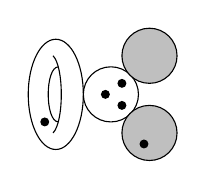
\begin{tikzpicture}[scale=.7]
\draw (0,0) circle (.5cm);
\draw[radius=2pt, fill=black] (.2,.2) circle;
\draw[radius=2pt, fill=black] (.2,-.2) circle;
\draw[radius=2pt, fill=black] (-.1,0) circle;

\draw[radius=2pt, fill=black] (-1.2,-.5) circle;
\draw[fill=gray!50] (.7,.7) circle (.5cm);
\draw[fill=gray!50] (.7,-.7) circle (.5cm);
\draw (-1,0) ellipse (.5cm and 1cm);
\draw (-1.05,.7) .. controls (-.85,.5) and (-.85,-.5) .. (-1.05,-.7);
\draw (-.95,.5) .. controls (-1.2,.5) and (-1.2,-.5) .. (-.95,-.5);
\draw[radius=2pt, fill=black] (.6,-.9) circle;
\end{tikzpicture}
\caption{``Mickey Mouse with an earring is eating a doughnut with a fly''}
\end{figure}

The local model for the space near such a boundary point is $V(xy,xz)\subseteq\Aaff^3_{x,y,z}$, where $D^1=\{x=0\}$ and $D^2=\{y=z=0\}$. The normal cone \[\Spec\left(\kk[x,y,z][A,B]/(xy,xz,zA-yB)\right)\] has two components defined by $(y,z)$ (this is a rank-two vector bundle on $D^2$, coinciding with its normal bundle) and $(x,zA-yB)$: the latter is \emph{not} a line bundle on $D^1$, as it has rank two over the origin, so in particular it is not its normal bundle; on the other hand the cycle of this cone has dimension three, and its restriction to the origin has dimension two, so we may effectively delete it, and behave \emph{as if} it were just the normal bundle of $D^1$. We may therefore argue as before, and we find that the relevant bundles are \[\frac{\mathbb E^\vee\boxtimes \ev_q^*T_{\PP^3}}{\mathbb L^\vee_{q,E}\boxtimes \mathbb L^\vee_{q,R}}\]
on $D^1$, of which we take $c_2$, while on $D^2$ we compute $c_1$ of \[\frac{\mathbb E^\vee\boxtimes \ev_q^*T_{\PP^3}}{\mathbb L^\vee_{q_1,E}\boxtimes \mathbb L^\vee_{q,R_1}\oplus\mathbb L^\vee_{q_2,E}\boxtimes \mathbb L^\vee_{q,R_2}}.\]
$D^3$ has dimension equal to the virtual dimension. A Chern class calculation implies (with schematic notation suggested by N. Nabijou):
\begin{multline*}
 \virt{\M{1}{n}{\PP^3}{d}}=[\reduced]+ 4[\Dunouno]+4[\Dunodue]+\\
 -3[\Dunotre]-3[\Dunoquat]+[\Dunocin]+2[\Dunosei]+\\
 [\Dunoset]+3[\Dunoott]-8[\Dunonov]+6[\Dunodiec]+\\
 4[\Ddueuno]-3[\Dduedue]+[\Dduetre]+[\Dduequat]+\\
 [\Dduecin]+[\Dduesei]+[\Dtre]
\end{multline*}
If we restrict our attention to primary invariants, the only survivors are:
\begin{multline*}
 [\reduced]+ 4[\Dunouno]-3[\Dunotre]-3[\Dunoquat]+\\
 [\Dunocin]+2[\Dunosei]+3[\Dunoott]-8[\Dunonov]
\end{multline*}
They contribute tidily as follows:
\begin{enumerate}
 \item gives the reduced invariants,
 \item $4\langle\psi\rangle_{1,1}\langle H,-\rangle^{\PP^3}_{0,n+1,d}=\frac{4d}{24} GW_0$ by divisor,
 \item $-3\langle\lambda_1\psi,1\rangle_{1,2}\langle -\rangle^{\PP^3}_{0,n,d}=\frac{-3n}{24} GW_0$ since there are $n$ choices for the marking on the genus one curve,
 \item $-3\langle\lambda_1\rangle_{1,1}\langle \psi,-\rangle^{\PP^3}_{0,n+1,d}=\frac{-3(n-2)}{24} GW_0$ by dilaton,
 \item $\langle\psi^2,1\rangle_{1,2}\langle -\rangle^{\PP^3}_{0,n,d}=\frac{n}{24} GW_0$,
 \item $2\langle\psi\rangle_{1,1}\langle \psi,-\rangle^{\PP^3}_{0,n+1,d}=\frac{2(n-2)}{24} GW_0$ by dilaton,
 \item vanishes since $\langle\lambda_1^2,1\rangle_{1,2}=0$,
 \item $-8\langle\lambda_1\rangle_{1,1}\langle H,-\rangle^{\PP^3}_{0,n+1,d}=\frac{-8d}{24} GW_0$ by divisor.
\end{enumerate}
Summing up we obtain the following:
\begin{prop}[Li-Zinger formula for primary insertions on $\PP^3$] \[\langle \delta_1,\ldots,\delta_n \rangle^{\PP^3}_{1,n,d}=\langle \delta_1,\ldots,\delta_n \rangle^{\PP^3,\mathrm{red}}_{1,n,d}+\frac{2-4d-3n}{24}\langle \delta_1,\ldots,\delta_n \rangle^{\PP^3}_{0,n,d}.\] \end{prop}
Notice that this differs from Li-Zinger's original formula by the contribution of the markings (which is not of interest in the CY3 case). An alternative approach would be to compare every boundary component to its genus zero relative by virtual pushforward: if we are only interested in primary insertions, notice that the components of $D^1$ such that more than one marking dwells on the elliptic curve will not contribute, since the excess bundle has rank two.

\section{Maps from curve singularities}\label{sec:singularities}
A different approach to reduce the complexity of $\M{1}{n}{\PP^N}{d}$ is the one followed by M. Viscardi in \cite{VISC}, building on work of D.I. Smyth on the minimal model program for $\oM_{1,n}$ \cite{SMY1}. Rather than blowing up and desingularising the main component, the idea is to collapse a number of boundary components, filling in their intersection with \emph{main} and the boundary components of smaller dimension. Vakil's description of the smoothable elements of $\M{1}{n}{\PP^N}{d}$ (see Proposition \ref{prop:components}(2)) suggests to do so by allowing maps from more singular (than nodal) curves, and simultaneously making their semistable models unstable, in order to preserve the separatedness of the moduli space.

The easiest example is the following: the cusp
\[\kk[\![x,y]\!]/(y^2-x^3)\]
is the only unibranch singularity of genus one (meaning that there exists a flat family of smooth elliptic curves degenerating to an irreducible curve of geometric genus $0$ and with only one singular point, around which the curve is formally isomorphic to the spectrum of the ring above). It is a well-known computation \cite[\S 3.C]{HM} that the semistable reduction of the cusp has a rational tail (normalising the singularity) attached to an elliptic curve at the preimage of the singular point; this indicates that we should make curves of genus one with only one special point unstable. On the other hand the only singularities appearing in the fibers of the miniversal deformation of the cusp are nodes, hence for a curve being \emph{at worst cuspidal} (i.e. smooth, nodal or cuspidal) is an open condition. Consider then the following:
\begin{dfn}
 The moduli space of $1$-stable maps $\Mone{n}{X}{\beta}$ parametrises $f\colon (C,\mathbf p)\to X$ such that
 \begin{enumerate}
  \item $C$ is an at worst cuspidal, projective curve of arithmetic genus one, and $\mathbf p$ is an $n$-tuple of smooth and disjoint sections of $C$;
  \item if $C_0$ is a minimal subcurve of $C$ contracted by $f$, the number of markings on $C_0$ added to the number of intersections of $C_0$ with $\overline{C\setminus C_0}$ is at least $3$ if $p_a(C_0)=0$, and \emph{at least $2$} if $p_a(C_0)=1$;
  \item $f_*[C]=\beta\in H^+_2(X)$ and $\Aut(C,f)$ is finite.
 \end{enumerate}
\end{dfn}
\begin{lemma}
 $\Mone{n}{X}{\beta}$ is a proper DM stack of finite type over $\kk$.
\end{lemma}
For example $\oM^{(1)}_1(\PP^2,3)$ only has two irreducible components, since there is no $D^1$ anymore. The intersection of $D^1$ with \emph{main} and with $D^2$ has been filled in with maps from cuspidal curves. This is the main instance of Smyth-Viscardi's spaces that I am going to be concerned with, but there is a well-developed theory which I shall quickly review here.
\subsection{Gorenstein singularities of genus one and $1$-stabilisation}
\begin{dfn}\label{def:genus}
 Let $(C,p)$ be the germ of a curve singularity, with normalisation $\nu\colon\widetilde{C}\to C$. Let me denote by $m$ the number of branches of $C$ at $p$ (i.e. irreducible components of $\widetilde{C}$) and by $\delta=\dim_{\kk}(\nu_*\OO_{\widetilde{C}}/\OO_C)$. The \emph{genus} of $(C,p)$ is defined by \[g=\delta-m+1.\]
\end{dfn}
\begin{prop}\cite[Proposition A.3]{SMY1}
 There is up to isomorphism only one germ of Gorenstein curve singularity $(C,p)$ of genus one with $m$ branches, namely
 \[\hat\OO_{C,p}\simeq\begin{cases} \kk[\![x,y]\!]/(y^2-x^3) & \text{(cusp) if } m=1, \\ \kk[\![x,y]\!]/y(y-x^2) &  \text{(tacnode) if } m=2,\end{cases}\]
 and the germ of $m$ generic lines through the origin in $\Aaff^{m-1}$ for $m\geq 3$. It is called the \emph{elliptic $m$-fold point}.
\end{prop}
All these singularities are smoothable (see the proof of \cite[Theorem 3.8]{SMY1}). Smyth studied their semistable models: pick a smoothing $\overline{\mathcal C}$ of the $m$-fold elliptic point and consider its semistable model with \emph{regular} total space $\widetilde{\mathcal C}$; let $(E,q_1,\ldots,q_m)$ be the exceptional locus of the contraction (the fiber over the $m$-fold elliptic point) marked with its intersection with the rest of the curve ($m$ rational trees). Call a semistable genus one curve $(E,q_1,\ldots,q_m)$ a \emph{semistable tail} if it arises in this way. Smyth shows \cite[Proposition 2.12]{SMY1} that semistable tails can be characterised combinatorially as those curves such that the distance (on the dual graph) from $q_i$ to the core of $E$ is constant for all $i=1,\ldots,m$ (\emph{balancing condition}). The idea is that $\overline{\mathcal C}$ is a normal surface, and it is Gorenstein if and only if the central fiber is. In this case, denoting by $\phi\colon \widetilde{\mathcal C}\to\overline{\mathcal C}$ the contraction, $\phi^*\omega_{\overline{\mathcal C}}=\omega_{\widetilde{\mathcal C}}(D)$ for some divisor $D$ supported on the exceptional locus $E$ and such that $\omega_{\widetilde{\mathcal C}}(D)_{|E}\simeq\OO_E$; we can find appropriate weights on the components of $E$ such that this holds precisely in the balanced case. On the other hand, if balancing holds, we may contract $E$ by applying the Proj construction to $\omega_{\widetilde{\mathcal C}}(D)$ (possibly twisted by some horizontal divisor away from $E$) as above, and then show that the resulting $\overline{\mathcal C}$ is Gorenstein by relating its dualising sheaf to the $\OO_{\overline{\mathcal C}}(1)$ given by the Proj construction. The Smyth's singularity one gets when contracting a balanced curve is determined by the number of rational trees attached to it,  which is exactly the number of branches of the singularity. These singularities have no moduli (on the other hand the global configuration of the curve may have moduli, i.e. the positioning of special points). This discussion indicates what are the stable curves/maps that we should make unstable in order to keep the moduli space separated. Before passing to maps, let me make a few remarks.

\begin{rmk}
 It is well known that the cusp is obtained by collapsing the double point in $\PP^1$, i.e. it is the pushout of the following diagram:
 \bcd
 \Spec k[\epsilon]\ar[r]\ar[d]\ar[dr,phantom,"\lrcorner"] & \Spec k\ar[d] \\
 (\PP^1,0)\ar[r] & (\overline C, \bar 0)
 \ecd
 where the vertical arrow on the left is any but the zero tangent vector. In fact a similar statement is true for every elliptic $m$-fold, which is the collapsing of a generic tangent vector at the \emph{rational} $m$-fold. At the level of algebra, this boils down to the statement that $\widehat\OO_{\overline C,\bar 0}= R\times_{k[\epsilon]} k$, where $R\subseteq \kk[\![t_1]\!]\oplus\ldots\oplus \kk[\![t_m]\!]$ is the subalgebra $\{(p_1,\ldots,p_m):\ p_1(0)=\ldots=p_m(0)\}$ and the map $R\to \kk[\epsilon]$ sends $(p_1,\ldots,p_m)$ to $\epsilon\sum_{i=1}^m p_i^\prime(0)$.
\end{rmk}

I will record here a useful fact for the study of maps to $\PP^N$ that descend to a Smyth's singularity. Observe that, if $\nu\colon (C,0)\to (\overline{C},\bar{0})$ is the semi-normalisation of a Gorenstein genus one singularity (i.e. $(C,0)$ is a \emph{rational} $m$-fold point, or the pushout of a point in $m$ copies of $\PP^1$), then $\nu^*\colon \Pic^{(d_1,\ldots,d_m)}(\overline{C})\to \{\OO_{C}(d_1,\ldots,d_m)\}$ has kernel isomorphic to $\mathbb G_a$. On the other hand the pullback of sections of a line bundle $\mathcal L$ of non-negative multidegree on $\overline{C}$ gives a hyperplane in $H^0(C,\OO_{C}(d_1,\ldots,d_m))$ by Riemann-Roch.
\begin{lemma}\label{lem:fundamental}
 Two sections $s$ and $t$ of $H^0(C,\OO_{C}(d_1,\ldots,d_m))$ descend to the same line bundle $\mathcal L$ on $\overline{C}$ if and only if they satisfy: \begin{equation}\label{eq:descending}s(0)\sum_{i=1}^m t_i^\prime(0)=t(0)\sum_{i=1}^m s_i^\prime(0).\end{equation}
\end{lemma}
\begin{proof}
 Notice that \eqref{eq:descending} is invariant under scaling on the line bundle fibers, as well as under automorphisms of the curve that fix $0$ (these act as scalar multiplication up to first order), so it does not depend on the choice of coordinates. Assume first that $t$ does not vanish at $0$. Then $s/t$ is a rational function on $C$ with poles away from $0$, so it must satisfy a linear condition on the derivatives along the different branches, which up to automorphisms of $C$ we may assume to be $\sum_{i=1}^m (s/t)_i^\prime(0)=0$; multiplying by $t(0)^2$ we get the desired equation. This defines a hyperplane inside $H^0(C,\OO_{C}(d_1,\ldots,d_m))$ and we can associate to it $\frac{1}{t(0)}\sum_{i=1}^m t_i^\prime(0)\in \mathbb G_a$. Otherwise assume that all the sections of $\mathcal L$ vanish at $\bar{0}$; then they have to do so to order higher than one, because $\bar{0}$ is not a Cartier divisor in $\overline{C}$, but this defines too small a subspace of $H^0(C,\OO_{C}(d_1,\ldots,d_m))$, hence there is no such an $\mathcal L$.
\end{proof}

\begin{rmk}
 The operation of collapsing elliptic tails to cusps ($1$-stabilisation) works well in families (in fact, even when the elliptic tail is a component of a curve of higher genus \cite{Schubert}). On the other hand, the $m$-stabilisation is not well-defined. Here is an example from \cite[Remark 4.12]{BCM}:
 \begin{figure}[h]
\centering
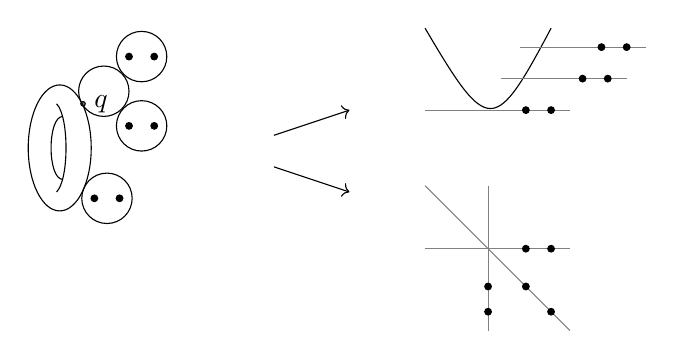
\begin{tikzpicture}[scale=.8]
\draw (-.1,0) circle (.4cm);
\draw[fill=gray] (-.43,-.20) circle[radius=1pt] node[right=.02cm]{$q$};
\draw (.5,.55) circle (.4cm);
\draw[fill=black] (.3,.55) circle[radius=1.5pt];
\draw[fill=black] (.7,.55) circle[radius=1.5pt];
%\node [above right] at (.8,.7) {$d_1$};
\draw (.5,-.55) circle (.4cm);
\draw[fill=black] (.3,-.55) circle[radius=1.5pt];
\draw[fill=black] (.7,-.55) circle[radius=1.5pt];
%\node [above right] at (.8,-.45) {$d_2$};
\draw (-.8,-.9) ellipse (.5cm and 1cm);
\draw (-.85,-.2) .. controls (-.65,-.4) and (-.65,-1.4) .. (-.85,-1.6);
\draw (-.75,-.4) .. controls (-1,-.4) and (-1,-1.4) .. (-.75,-1.4);
\draw (-.05,-1.7) circle (.4cm);
\draw[fill=black] (.15,-1.7) circle[radius=1.5pt];
\draw[fill=black] (-.25,-1.7) circle[radius=1.5pt];
%\node [above right] at (.25,-1.8) {$d_3$};

\draw[->] (2.6,-.7) -- (3.8,-.3);
\draw[->] (2.6,-1.2) -- (3.8,-1.6);

\draw[gray] (5,-.3)-- (7.3,-.3);
\draw[fill=black] (7,-.3) circle[radius=1.5pt];
\draw[fill=black] (6.6,-.3) circle[radius=1.5pt];
%\node [right] at (7,-.2) {$d_3$};
\draw (5,1) .. controls (6,-.7) and (6.1,-.7) .. (7,1);
\draw[gray] (6.5,.7)-- (8.5,.7);
\draw[fill=black] (7.8,.7) circle[radius=1.5pt];
\draw[fill=black] (8.2,.7) circle[radius=1.5pt];
%\node [right] at (8.5,.8) {$d_1$};
\draw[gray] (6.2,.2)-- (8.2,.2);
\draw[fill=black] (7.5,.2) circle[radius=1.5pt];
\draw[fill=black] (7.9,.2) circle[radius=1.5pt];
%\node [right] at (8.2,.3) {$d_2$};

\draw[gray] (5,-2.5)-- (7.3,-2.5);
\draw[fill=black] (7,-2.5) circle[radius=1.5pt];
\draw[fill=black] (6.6,-2.5) circle[radius=1.5pt];
%\node [right] at (7,-2.4) {$d_3$};
\draw[gray] (6,-1.5)-- (6,-3.8);
\draw[fill=black] (6,-3.5) circle[radius=1.5pt];
\draw[fill=black] (6,-3.1) circle[radius=1.5pt];
%\node [right] at (6.2,-1.5) {$d_2$};
\draw[gray] (5,-1.5)-- (7.3,-3.8);
\draw[fill=black] (7,-3.5) circle[radius=1.5pt];
\draw[fill=black] (6.6,-3.1) circle[radius=1.5pt];
%\node [right] at (7,-3.4) {$d_1$};
\end{tikzpicture}
\caption{Two different plausible $3$-stabilisations.}
\end{figure}
the curve on the left is not $3$-stable. We could contract the maximal unpointed subcurve of genus one, but it is not balanced; on the other hand, say we could consistently contract the minimal genus one subcurve: by smoothing the node $q$ and doing so, we would get a family of $3$-fold elliptic points specialising to the tacnode, which can be excluded by studying the miniversal deformation of the latter. This problem is studied in \cite[\S 4.1]{SMY2}. \end{rmk}
I will discuss a specific variation on this \cite[Theorem 4.4]{BCM} that I am going to need later. Recall that $\mathfrak M_{1}^{\operatorname{wt}=d,\text{st}}$ is the open and bounded substack within the Artin stack of prestable curves with a weight assignment, defined by the conditions that the total weight is $d$ and the curve is weighted-stable; similarly $\mathfrak M_{1}^{\operatorname{wt}=d,\text{st}}(1)$ is the stack of weighted $1$-stable (at worst cuspidal) curves.
\begin{prop}\label{prop:1-stab}
There exists a morphism $\mathfrak M_{1}^{\operatorname{wt}=d,\text{st}}\to\mathfrak M_{1}^{\operatorname{wt}=d,\text{st}}(1)$ which extends the identity on the smooth locus.
\end{prop}

The proof is inspired by \cite[\S2]{HassettHyeon} and \cite[\S3.7]{RSPW}. We construct the contraction over $\MM_1^{\rm{div}}$ (the moduli space of nodal curves of genus one with a simple smooth divisor of total degree $d$ that makes them weighted-stable) first, and then show that it descends to $\MM_1^{\rm{wt,st}}$. We work on $\MM_1^{\rm{div}}$ in order to have a natural polarisation.

Let $\pazocal E$ be the locus inside the universal curve over $\MM^{\rm{wt,st}}_1$ spanned by elliptic tails of weight $0$; this is a Cartier divisor, and abusing notation I will denote by $\pazocal E$ all its pullbacks. Moreover let $\mathfrak D^1$ be its image in $\MM^{\rm{wt,st}}_1$, which is a Cartier divisor as well.

Consider the following line bundle on the universal curve over $\MM_1^{\rm{div}}$: 
\begin{equation*}\label{eq:linebundlecontraction}
\mathcal N:=\omega_{\pi}(\pazocal E)\otimes\mathcal O_{\cC}(2\pazocal D),
\end{equation*} where $\pazocal D$ is the universal Cartier divisor over $\MM_1^{\rm{div}}$.

\begin{prop}\label{1-stabilization-div}
Let $\hC=\underline{\operatorname{Proj}}_{\MM_1^{\rm{div}}}(\bigoplus_{n\geq 0}\pi_*\mathcal N^{\otimes n})$. Then $\hC$ is a family of weighted $1$-stable curves and $\phi$ is a regular morphism:
 
 \bcd
 (\cC,\pazocal D)\ar[rr,"\phi"]\ar[dr,"\pi"] & & (\hC,\phi(\pazocal D))\ar[ld,"\bar{\pi}" above left] \\
 & \MM_1^{\rm{div}} &
 \ecd
This defines the $1$-stabilisation morphism $\MM_1^{\rm{div}}\to\MM_1^{\rm{div}}(1)$.
\end{prop}

Notice that $\mathcal N$ is trivial on the locus of elliptic tails, so this will be contracted by $\phi$. We need to prove that $\mathcal N$ is $\pi$-semiample (regularity of $\phi$) and that $\pi_*\mathcal N$ is locally free (flatness of $\bar{\pi}$). This is clear on the smooth locus; to prove it along $\mathfrak D^1$ we use \cite[Lemma~3.7.2.2]{RSPW}.
\begin{lem}[Pullback with a boundary]\label{DVR}
Let $\pi\colon\cC\to S$ be a proper family of curves over a smooth basis, and let $\mathcal N$ be a line bundle on $\cC$ such that $\operatorname{R}^1\pi_*\mathcal N$ is a line bundle supported on a Cartier divisor $\mathfrak D\subseteq S$. Then for every DVR scheme $\dvr$ with closed point $0$ and generic point $\eta$, and for every morphism $f\colon \dvr\to S$ such that $f(0)\in\mathfrak D$ and $f(\eta)\in S\setminus\mathfrak D$ we have
\[f^*\pi_*\mathcal N\cong \pi_{\dvr,*}f_\cC^*\mathcal N.\]
\end{lem}

\begin{lem}\label{lemma:semiample}
The line bundle $\mathcal N$ is $\pi$-semi-ample, i.e. the natural map
\[\pi^*\pi_*\mathcal N^{\otimes n}\to \mathcal N^{\otimes n}\]
is surjective for $n\gg 0$.
\end{lem}
\begin{proof}
Outside the locus of elliptic tails $\mathcal N$ is $\pi$-ample. We are left with checking at points of an elliptic tail; thanks to the above Lemma we can reduce to the case that $C$ is the central fiber of a one-parameter smoothing with regular total space. The fact is then proved within Smyth's contraction lemma \cite[Lemma~2.12]{SMY1}.
\end{proof}

\begin{lem}
$\pi_*\mathcal N$ is locally free on $\MM_1^{\rm{div}}.$
\end{lem}
\begin{proof} Compare with \cite[Proposition~3.7.2.1]{RSPW}.
We check that $\pi_*\mathcal N$ has constant rank.
On $\MM_1^{\rm{div}}\setminus \mathfrak{D}^1$, $\operatorname{R}^1\pi_*\mathcal N=0$, so $\pi_*\mathcal N$ satisfies Cohomology and Base Change \cite[Theorem III.12.11]{HAR} and its rank is determined by Riemann-Roch, hence constant.
Given a point $x$ on the boundary $\mathfrak{D}^1$, we can pick a one-parameter smoothing as above, and we can check the rank at $x$ by looking at $\pi_*f^*\mathcal N$ over $\dvr.$ Now $f^*\mathcal N$ is flat over $\dvr$, so $\pi_*f^*\mathcal N$ is as well, which implies torsion-free and thus constant rank.
\end{proof}

\begin{proof}\eqref{1-stabilization-div}
Let $S\to \MM_1^{\rm{div}}$ be a smooth atlas, then we have:
 \bcd
 (\cC_S,\pazocal D_S)\ar[rr,"\phi_S"]\ar[dr,"\pi_S"] & & (\hC_S,\phi(\pazocal D_S))\ar[ld,"\bar{\pi}_S" above left] \\
 & S &
 \ecd
where $\hC_S=\underline{\operatorname{Proj}}_{S}(\bigoplus_{n\geq 0}\pi_{S,*}\mathcal N^{\otimes n})$, $\phi_S$ is a proper and birational, and $\bar{\pi}_S$ is a flat family. 
To verify that this defines a morphism $S\to \MM_1^{\rm{div}}(1)$ we have to argue that $\hC_S$ has reduced fibers and only nodes and cusps as singularities. After pulling back to a generic $\dvr$, this is again Smyth's contraction lemma \cite[Lemma~2.13]{SMY1}. $\mathcal D$ is pushed forward along $\phi$ and it satisfies weighted-stability, since $\phi$ is an isomorphism outside the locus of elliptic tails. To conclude that this defines a morphism $\MM_1^{\rm{div}}\to \MM_1^{\rm{div}}(1)$ it is enough to verify that there is an isomorphism
 $\rm{pr}_1^*\hC_S\cong\rm{pr}_2^*\hC_S$ satisfying the cocycle condition, where $\rm{pr}_i\colon S'= S\times_{\MM_1^{\rm{div}}} S\rightrightarrows S$.%and that $\rm{pr}_{ij}\colon S\times_{\MM_1^{\rm{div}}} S\times_{\MM_1^{\rm{div}}} S\to  S\times_{\MM_1^{\rm{div}}} S $ satisfy the cocycle condition.

 Now $\pr_i^*\hC_S$ is obtained by applying the Proj construction to 
 $\rm{pr}_i^*(\pi_{S,*}\mathcal{N})\cong\pi_ {S',*} (\rm{pr}_i^*\mathcal N)$, which are isomorphic because $S'\to S$ is flat. On the other hand $\rm{pr}_1^*\mathcal N\cong \rm{pr}_2^*\mathcal N$ since $\mathcal N$ is the pullback of a line bundle on $\MM_1^{\rm{div}}$. The cocycle condition is derived similarly. 
\end{proof}


\begin{lemma}
The $1$-stabilisation for curves with a divisor induces an analogous morphism at the level of weighted curves:
\bcd
\MM_1^{\rm{div}}\ar[r]\ar[d]\ar[dr,phantom,"\circlearrowright"] & \MM_1^{\rm{div}}(1)\ar[d] \\
\MM_1^{\rm{wt,st}}\ar[r,"\exists"] & \MM_1^{\rm{wt,st}}(1)
\ecd
\end{lemma}
\begin{proof}
{\'E}tale locally on $\MM_1^{\rm{wt,st}}$ we can choose smooth sections $s_i$ of the universal curve so that the Cartier divisor $\pazocal D=\sum s_i$ has degree compatible with the weight function, so in particular it makes $\mathcal N=\omega_{\pi}(\pazocal E)\otimes\mathcal O_{\cC}(2\pazocal D)$ trivial on the elliptic tails and $\pi$-ample elsewhere.
For a smooth atlas $S\to \MM_1^{\rm{wt,st}}$, this observation allows us to define a lifting $S\to \MM_1^{\rm{div}}$, and thus a morphism $\xi\colon S\to  \MM_1^{\rm{wt,st}}(1)$ via the construction of Proposition \ref{1-stabilization-div}.

In order to show that this descends to a morphism $\MM_1^{\rm{wt,st}}\rightarrow \MM_1^{\rm{wt,st}}(1)$ we need to verify that there exists $\rm{pr}_1^*(\xi)\cong\rm{pr}_2^*(\xi)$ satisfying the cocycle condition, where $\rm{pr}_i\colon S'= S\times_{\MM_1^{\rm{wt,st}}} S\rightrightarrows S$.

This boils down to checking that for two different choices of a lifting $\pazocal D_1,\pazocal D_2\colon S\to\MM_1^{\rm{div}}$ there exists a unique isomorphism 
\[\hC_1=\underline{\operatorname{Proj}}_S\left(\bigoplus_{n\geq 0}\pi_*(\mathcal N_1^{\otimes n})\right)\cong \underline{\operatorname{Proj}}_S\left(\bigoplus_{n\geq 0}\pi_*(\mathcal N_2^{\otimes n})\right)=\hC_2. \]
By construction there is a birational map $\psi$:
 \bcd
&\cC_S \ar[dl,"\phi_1" above left]\ar[dr,"\phi_2"]  \\
 \hC_1\ar[rr,dashed, "\psi"] & &\hC_2.
 \ecd

We want to show that $\psi$ extends to a regular morphism. 
Notice that $ \hC_i$ is normal, $i=1,2$: indeed since $S$ is smooth and the singularities of the fibers are in codimension $1$, $ \hC_i$ is regular in codimension $1$; since both $S$ (smooth) and the fibers (Cohen-Macaulay) satisfy Serre's condition $S_2$, so does the total space of $\hC_i$ by \cite[Theorem~23.9]{MAT}. By Zariski's connectedness theorem $\phi_{i,*}\OO_{\cC_S}\cong \OO_{\hC_i}$.
By construction $\operatorname{Exc}(\phi_1)=\operatorname{Exc}(\phi_2)$ is the locus of elliptic tails of weight $0$, so in particular $\phi_2$ contracts all the fibers of $\phi_1$. Then \cite[Lemma 1.15]{debarre}
implies that $\phi_2$ factors through $\phi_1$, and viceversa. This proves the regularity of $\psi$ and its inverse. Notice that $\psi$ is unique as it is the only extension of $\phi_2\circ\phi_1^{-1}$.
\end{proof} 

This concludes the proof of Proposition \ref{prop:1-stab}.

\subsection{Viscardi's moduli spaces of maps} I finally come to M. Viscardi's definition of alternative compactification of the space of maps from a smooth elliptic curve \cite[Definition 2.15]{VISC}.

\begin{dfn}
 The moduli space of $m$-stable maps $\oM^{(m)}_{1,n}(X,\beta)$ parametrises $f\colon (C,\mathbf p)\to X$ of class $\beta$ such that:\begin{enumerate}
                                                                                                                                      \item $C$ has only nodes and $l$-fold elliptic points as singularities, with $l\leq m$, $p_a(C)=1$ and $\mathbf{p}=(p_1,\ldots,p_n)$ are smooth and disjoint sections,
                                                                                                                                      \item if $E\subseteq C$ is a connected subcurve contracted by $f$, and $p_a(E)=1$, then its \emph{level} is \[\lvert \{i\in[n]:\ p_i\in E\}\rvert+\lvert E\cap \overline{C\setminus E}\rvert >m,\]
                                                                                                                                      \item $\lvert\Aut(C,f)\rvert<+\infty$.
                                                                                                                                     \end{enumerate}

\end{dfn}
The usual Behrend-Fantechi's construction \cite[Proposition 6.2]{BF} endows $\oM^{(m)}_{1,n}(X,\beta)$ with a virtual class of the usual dimension. Setting $m=0$ recovers the usual space of Kontsevich's stable maps.

\begin{prop}\cite[Theorem 3.6]{VISC}
 $\oM^{(m)}_{1,n}(X,\beta)$ is a proper DM stack of finite type over $\kk$.
\end{prop}
Checking the valuative criterion for properness goes as follows: assume the generic fiber is smooth (in general we may work componentwise on the generic fiber); we may first complete the family over $\dvr$ as an ordinary stable map. If $f$ contracts the core and it does not satisfy $m$-stability, we can make it into doing so by a sequence of operations: alternate between contracting the core to a Smyth's singularity and \emph{sprouting}, i.e. blowing up at markings or nodes along the core. Notice that more sprouting may be required in order for the map to descend to the singularity (see \cite[Remark 2.6]{BCM}).

As anticipated, Viscardi's moduli space of $m$-stable maps to $\PP^N$ ``collapses'' the boundary components $D^k_1(\PP^N,d)$ for $k\leq m$ (the pointed case is subtler, as usual), hence the following result \cite[Corollary 5.10]{VISC}.
\begin{prop}
 There exists an $m_0=m_0(d,n)$ such that, for $m\geq m_0$, $\oM^{(m)}_{1,n}(\PP^N,d)$ is irreducible.
\end{prop}
\subsection{Aligned log structures and factorisation} Finally, I would like to discuss how these two lines of thought (Li-Vakil-Zinger's desingularisation and reduced invariants, compared to Smyth-Viscardi's alternative compactifications) are not unrelated. A main issue with the Vakil-Zinger desingularisation is that the iterated blow-up procedure makes the modular interpretation of the resulting space not so immediately clear. This has been recently fixed by D. Ranganathan, K. Santos-Parker and J. Wise with the introduction of the notion of an \emph{aligned} log curve. Recall the description of log smooth curves, due to F. Kato \cite{KatoF}, and the parallel with marked prestable curves. Let us work over a geometric point $S=\Spec(\kk=\bar\kk)$, and assume we have a log smooth curve of genus one $(C,\mathcal M_C)\to(S,\mathcal M_S)$. We can modify the usual dual graph construction by collapsing all the vertices corresponding to components of the core (in case the latter is a circle of $\PP^1$) to one vertex, called the \emph{circuit} and denoted by $\circ$. Define a piecewise-linear $\oM_S$-valued function on the dual graph $\Gamma(C)$ by \[\lambda(v)=\sum_{e\in[\circ,v]}\rho_e,\] i.e. by associating to a vertex/component the sum of all the smoothing parameters of the edges/nodes separating it from the circuit.
\begin{dfn}
 Let $S$ be a log scheme and $C\to S$ a family of log smooth curves of genus one. We say that $C$ is \emph{radially aligned} if for every geometric point $s\in S$ the values of $\lambda(v)$ are \emph{comparable} in $\oM_{S,s}$ for every vertex $v$ of $\Gamma(C_s)$, with respect to the partial order $m_1\leq m_2$ if there is $m_{1-2}\in\oM_{S,s}$ such that $m_1+m_{1-2}=m_2$.
\end{dfn}
There exist \emph{minimal} radially aligned log structures, hence the moduli problem over $(LogSch)$ is the enhancement of a moduli stack over $(Sch)$ endowed with a log structure, after work of D. Gillam \cite{Gillam}. At this level
\[\MM^{\mathrm{rad}}_{1,n}\to\MM_{1,n}\]
is a log modification, due to the key observation that a log blow-up along a log ideal $K$ determines on every one of its charts a minimal element among the generators of $K$, hence a sequence of log blow-ups will serve the goal of ordering a collection of sections of $\oM_S$ \cite[Lemma 3.36]{Kelithesis}. Pictorially, it corresponds to a subdivision of the dual minimal monoid (see \cite[\S 3.3-3.4]{RSPW}). On the other hand, for every \emph{stable} radially aligned curve over a geometric point $S$, and for every integer $m\geq0$, we may find a section $\delta_m$ of $\oM_S$ such that $\delta_m=\lambda(v)$ for some vertex of $\Gamma(C)$, and the circle of radius $\delta_m$ has inner valence less than $m$ and outer valence strictly larger than $m$. $\delta_m$ behaves well under specialisation/generisation, by semicontinuity of the inner and outer valence \cite[Proposition 3.5.2]{RSPW}, hence it can be defined over any base. The power of log structures is two-fold at this point:
\begin{enumerate}
 \item it produces a log-modification $\widetilde{C}\to C$ by subdividing the edges where they meet the circle of radius $\delta_m$ (i.e. blowing up some nodes and markings on the components with $\lambda(v)<\delta_m$) \cite[Proposition 3.6.1]{RSPW};
 \item by combining $\lambda$ and $\delta_m$, it produces a $\tilde{\pi}$-semiample line bundle on $\widetilde{C}$, the morphism associated to which contracts the strict interior of the circle of radius $\delta_m$, producing a diagram, with $\bar{\pi}\colon\overline{C}\to S$ an $m$-stable Smyth's curve \cite[Proposition 3.7.3.1]{RSPW}:
 \bcd[cramped]
 & \widetilde{C}\ar[dl]\ar[dr] & \\
 C\ar[dr,"\pi"] & & \overline{C}\ar[dl,"\bar{\pi}"] \\
 & S &
 \ecd
\end{enumerate}
\begin{rmk}
 It may seem that this construction sometimes happens to contract unbalanced curves, but it is not the case; notice that the blow-ups in point (1) above may occur along non-reduced centers. In fact, the strict interior of a circle around the circuit is the correct generalisation of a balanced elliptic tail when $C\to S$ is not just a one-parameter smoothing with regular total space.
\end{rmk}
This construction in the stable case provides a resolution of indeterminacy of the birational map between different Smyth's compactifications:
\bcd[cramped]
& \oM_{1,n}^{\mathrm{rad}}\ar[dr]\ar[dl] & \\
\oM_{1,n} \ar[rr,dashed] & & \oM_{1,n}^{(m)}
\ecd
More to the point, there is an extension of this construction to the realm of maps.
\begin{dfn}
 A \emph{centrally aligned map} $f\colon(C,\mathbf p)\to X$ over $S$ is a log morphism (where $X$ has the trivial log structure) with a section $\delta_0$ of $\oM_S$, such that $\delta_0=\lambda(v)$ for $v$ of minimal distance to the circuit among the non-contracted components, $\lambda(w)$ is comparable with $\delta_0$ for every $w$, and the $\lambda(w)$ are comparable with one another whenever they are smaller than $\delta_0$.
\end{dfn}
The section $\delta_0$ together with $\lambda$ defines a modification $\widetilde{C}$ and a contraction to $\overline{C}$ with a Smyth's singularity as above.
\begin{dfn}
 A centrally aligned map satisfies the \emph{factorisation property} if its pullback to $\widetilde{C}$ descends to $\overline{C}$:
 \bcd[cramped]
 & \widetilde{C}\ar[dl]\ar[dr] & \\
 C\ar[dr,"f"] & & \overline{C}\ar[dl,dashed,"\exists\bar{f}"] \\
 & X &
 \ecd
\end{dfn}
\begin{thm}\cite[Theorems 4.6.3.2 and 4.5.1]{RSPW}
 The moduli space of centrally aligned maps to projective space is isomorphic to the Vakil-Zinger blow-up. The factorisation property identifies the main component.
\end{thm}
Notice that by construction $\bar{f}$ is non-constant on at least one branch of the core. For every Gorenstein curve of genus one with no separating nodes, the dualising sheaf is trivial \cite[Lemma 3.3]{SMY1}. Therefore $H^1(\overline{C},\bar{f}^*\OO_{\PP^N}(1))=0$ by Serre duality, and the projection to $\MM^{\mathrm{cen}}_{1,n}$ is unobstructed (a perfect obstruction theory is given by $\R\bar{\pi}_*\bar{f}^*T_{\PP^N}$), so every element satisfying factorisation is smoothable; on the other hand factorisation is a closed condition \cite[Theorem 4.3]{RSPW}. This proves the second claim.

\begin{rmk}
 From the discussion above we see that the construction in \cite{RSPW} might be suitable to extend the definition of reduced invariants to a larger class of varieties than projective complete intersections. It is enough that $\VZ{n}{X}{\beta}$ is irreducible and $Y\subseteq X$ is such that $N_{Y/X}$ is an ample vector bundle, so that $\operatorname R^1\bar{\pi}_*\bar{f}^*N_{Y/X}=0$ and the inclusion $\VZ{n}{Y}{\beta}\hookrightarrow\VZ{n}{X}{\beta}$ admits a perfect obstruction theory. On the other hand if we want to prove that $\VZ{n}{X}{\beta}$ is smooth following in the steps above, we need $T_X$ ample, which is quite a restrictive condition (the only smooth variety with ample tangent bundle is the projective space, by a theorem of Mori \cite{Mori}, on the other hand it could be possible e.g. to extend to the orbifold theory of weighted projective spaces).
\end{rmk}
\subsection{Reduced vs cuspidal invariants} In the next section I am going to discuss a result that I have obtained with F. Carocci and C. Manolache, which illustrates the relation between the Li-Vakil-Zinger's and the Smyth-Viscardi's projects under a slightly different light: namely, the idea is that the reduced invariants may be recovered as $m$-stable invariants, whenever $m$ is big enough that all the boundary components contributing non-trivially to the right hand side of the Li-Zinger's formula have been collapsed. We demonstrate this principle in the case of the quintic threefold, for which only $D^1$ matters, so that it is enough to allow maps from cuspidal curves.

\begin{thm}\cite{BCM}\label{thm:redvscusp}
 For a smooth quintic threefold $X_5=V(\mathbf w)\subseteq \PP^4$, \[GW_1^{\mathrm{red}}(X_5)=GW_1^{(1)}(X_5).\]
\end{thm}
This is really a result about the virtual cycles, hence it holds for any (descendant) insertion. Here is an idea of how the proof could go: recall from Proposition \ref{prop:1-stab} that there is a well-defined $1$-stabilisation morphism at the level of weighted-stable curves; the following fiber product
\bcd
\mathcal Z_X\ar[r,"\alpha"]\ar[d]\ar[dr,phantom,"\Box"] & \oM^{(1)}(X_5,d)\ar[d] \\
\mathfrak M_{1}^{\operatorname{wt}=d,\text{st}}\ar[r] & \mathfrak M_{1}^{\operatorname{wt}=d,\text{st}}(1)
\ecd
is endowed with a class $\virt{\mathcal Z_X}$ by virtual pullback, such that $\alpha_*\virt{\mathcal Z_X}=\virt{\oM^{(1)}(X_5,d)}$, because $\mathfrak M_{1}^{\operatorname{wt}=d,\text{st}}\to \mathfrak M_{1}^{\operatorname{wt}=d,\text{st}}(1)$ is proper \cite[Lemma 4.19]{BCM} and birational, and by commutativity of virtual pullbacks with proper pushforward \cite{Manolache-Pull}. On the other hand there is a closed embedding of $\mathcal Z_X$ into ordinary stable maps $\oM_1(X,d)$ \cite[Lemma 4.13]{BCM}; it is an isomorphism with the substack of maps satisfying factorisation through the $1$-stabilisation of the underlying weighted curve. In particular $\mathcal Z_X$ has a main component, and all the boundary components except $D^1(X,d)$. Unfortunately it is hard to study the intrinsic cone of $\oM_1(X,d)$ directly, hence we resort to an indirect approach, extending work of H.L. Chang, Y. Hu, Y.-H. Kiem and J. Li to the situation at hand.

\subsection{A word on genus two}

This section is based on discussions I have had with F. Carocci. The geometry of the moduli space of maps of genus two to $\PP^N$ is more complicated than that of genus one. A key focus of recent research has been towards verifying the \cite{BCOV} prediction for the higher genus Gromov-Witten potential (of the quintic threefold). Zinger managed to do so in genus one \cite{Zinger-CYhyp}, as the culmination of the articulate project I have tried to outline in the previous sections. An approach to the genus two case \`a la Li-Vakil-Zinger, i.e. through a partial desingularisation of the moduli space, has been attempted by Hu and Li in \cite{HL2}: it is quite subtle, even though incomplete, and it appears to have remained dormant for more than five years now. On the other hand there has been a recent breakthrough, due to S. Guo, F. Janda, and Y. Ruan \cite{GJR}, based on torus localisation on a compactification - inspired by the theory of log stable maps - of the moduli space of maps with $p$-fields (in fact of a more general GLSM moduli space \cite{CJRS}). Nonetheless I believe it would be relevant to gain a better understanding of the geometry of the moduli space of maps, possibly with a view towards the definition of reduced invariants, which should provide a modular definition of BPS numbers \cite{PandhaHodge}, at least under some extra hypotheses (e.g. the curve class is primitive).

Following Smyth's procedure in \cite[Appendix A]{SMY1}, we are able to classify the unibranch singularities of genus two. Let $(R,\m)$ be the completion of the local ring of the curve at the singularity, with normalisation:
\[(\tR,\tm)\simeq\left(\kk[\![t_1]\!]\oplus\ldots\oplus\kk[\![t_m]\!],\langle t_1,\ldots,t_m\rangle\right).\]
So $m$ is the number of branches, and $\delta=m+1$ for $g=2$ (compare with Definition \ref{def:genus}). It is an observation of Smyth's that $\tR/R$ is graded by:
\[ (\tR/R)_i:=\tm^i/(\tm^i\cap R)+\tm^{i+1};\]
furthermore he notices that:
\begin{enumerate}
\item $m+1=\delta(p)=\sum_{i\geq 0}\dim_\kk(\tR/R)_i;$
\item $2=g=\sum_{i\geq 1}\dim_\kk(\tR/R)_i;$
\item if $(\tR/R)_i=(\tR/R)_j=0$ then $(\tR/R)_{i+j}=0$.
\end{enumerate}
The following facts will also turn out to be useful:
\begin{enumerate}[resume]
 \item $\sum_{i\geq k}(\tR/R)_i$ is a grading of $\tm^k/(\tm^k\cap R)$;
 \item there is an exact sequence:
 \[ 0\to \frac{\tm^k\cap R}{\tm^{k+1}\cap R}\to \frac{\tm^k}{\tm^{k+1}}\to \left(\tR/R\right)_k\to 0.\]
\end{enumerate}

Notice that in the unibranch case $\dim_\kk(\tR/R)_1\leq 1$, hence equality must hold (by observation (3) above). We are thus left with two cases:
 \begin{enumerate}
  \item either $\dim_\kk(\tR/R)_2=1$ and $\dim_\kk(\tR/R)_i=0$ for all $i\geq 3$: in this case $\tm^3\subseteq\m$ by observation (4). Indeed we see by (5) that \[\tm^3=\m,\] hence $R\simeq\kk[\![t^3,t^4,t^5]\!],$ a non-Gorenstein singularity.
  
  \item or $\dim_\kk(\tR/R)_3=1$ and $\dim_\kk(\tR/R)_i=0$ for $i=2$ and for all $i\geq 4$: in this case $\tm^4\subseteq\m$ by observation (4). On the other hand from $\dim_\kk(\tm^2\cap R/\tm^3\cap R)=1$ we deduce that there is a generator of degree $2$, and from $\dim_\kk(\tm^3\cap R/\tm^4\cap R)=0$ there is none of degree $3$; so we see that \[\m/\m^2=\langle t^2,t^5\rangle,\] i.e. $R\simeq\kk[\![x,y]\!]/(x^5-y^2)$, which is planar (hence Gorenstein).
 \end{enumerate}

We can show that the semistable models are as follows:
 \begin{enumerate}
  \item the non-Gorenstein singularity is obtained by collapsing a genus two tail which is attached to a rational tree at a non-Weierstrass point;
  \item the planar singularity is obtained by collapsing a genus two tail which is attached to a rational tree at a Weierstrass point.
 \end{enumerate}
The idea is again that the normal surface you get after contracting is Gorenstein if and only if it has Gorenstein central fiber, if and only if the line bundle used to perform the contraction may be written as $\omega_{\mathcal C}(D)$ with $D$ supported on the exceptional locus, and such that $\omega_{\mathcal C}(D)_{|\operatorname{Exc}(\phi)}$ is trivial.

\begin{rmk}
 It was pointed out by D.I. Smyth that we cannot always construct simultaneous smoothings of the singularity and a semistable curve mapping to it (compare with \cite[Lemma 2.11]{BCM}). In particular it will not be true that any map that factors through a genus two singularity (and does not contract all of its branches) is automatically smoothable. Consider the map $f_0\colon\PP^1\to\PP^3$ given in coordinates by \[ [s:t]\mapsto[s^3t^2:t^5:st^4:s^5].\]
 It is the normalisation of a curve with a singularity of type (2) above. Now attach a genus two curve with a non-Weierstrass point to $(\PP^1_{[s:t]},[1,0])$, and let it be collapsed by the map. Assume the resulting genus two stable map were smoothable: then, by pulling back $\OO_{\PP^3}(1)$ and taking the relative Proj construction, we would get a family $\overline{\mathcal C}$ with central fiber of type (1), and such that the map $f\colon\mathcal C\to\PP^3$ factors through $\overline{\mathcal C}$. But this map should restrict to an isomorphism of the central fiber with its image (because it is birational, and the two curves have the same normalisation and $\delta$-invariant), which is a contradiction.
\end{rmk}

\begin{rmk}
 There are a number of genus two singularities with two branches. The complexity of carrying out an algebraic study as above increases steeply with the number of branches. On the other hand every genus two singularity with two branches is obtained by gluing two singularities $R_1$ and $R_2$ with $g(R_i)\leq 2$ along a closed subscheme of length $\leq 3$.
 This is clear if we look at the factorisation of the normalisation $R\hookrightarrow \widetilde{R}=k[\![t_1]\!]\oplus k[\![t_2]\!]$ through $R\hookrightarrow R_1\oplus R_2\hookrightarrow \widetilde{R},$ where 
 the first partial normalisation corresponds to separating the branches. Algebraically, this can be achieved by considering the quotient $K^{\rm{br}}$ of $\widetilde{R}/R$ generated by those conditions involving only one branch at the time, and then taking the kernel of $\widetilde{R}\to K^{\rm{br}}.$ For example $\kk[\![x,y]\!]/(y(x^3-y))$ is obtained by gluing two smooth branches. Compare with \cite[Appendix A]{SMYtowards}.
\end{rmk}

Finally, the components of $\M{2}{n}{\PP^N}{d}$, $d\geq 3$, are included in the following list (I will not mention the various possible distributions of the markings, and I will represent the decorated dual graph of a general element of each component):
\begin{enumerate}
 \item \emph{main} is the closure of the locus of maps from a smooth curve of genus two;
 \item $\mathcal D^k=\left\{\Dk\right\}$
  \item $\mathcal D^{\rm{hypell},k}=\left\{\hypell\right\}$
 \item $\mathcal E^k=\left\{\Ek\right\}$
 \item $\mathcal E^{(k_1,k_2)}=\left\{\Ekk\right\}$
 \item $\mathcal E^{\rm{nct}}=\left\{\pacman\right\}$
\end{enumerate}
Here is a funny example: consider $\oM_2(\PP^1,3)$. From the theory of limit linear series \cite{EH}, no element of $\mathcal D^{\rm{hypell},1}$ is smoothable: let the underlying curve be $Z\coprod_q R$, where $Z$ has genus two and $R\simeq\PP^1$. The aspect of the linear series supported on $Z$ is $\omega_Z(q)$, with vanishing sequence $(1,3)$ (if $q$ Weierstrass) and $(1,2)$ (otherwise), so the aspect $\mathcal L$ supported on $R$ has vanishing sequence $(0,2)$ or $(1,2)$; in any case $\mathcal L(-2Z)$ has only one section, so it cannot give a map to $\PP^1$. On the other hand $\mathcal D^{\rm{hypell},1}$ intersects $\mathcal D^2$, $\mathcal D^3$, $\mathcal E^1$, $\mathcal E^{0,1}$, $\mathcal E^{0,2}$, and $\mathcal E^{1,1}$. 

\section{p-fields, local equations and a splitting of the cone}\label{sec:techniques}

The indirect approach to the proof of Theorem \ref{thm:redvscusp} can be outlined as follows: we introduce the moduli space of $1$-stable maps with $p$-fields, $\oM_1^{(1)}(\PP^4,d)^p$, the geometry of which is closely related to that of $\oM_1^{(1)}(\PP^4,d)$ (in fact, it is a line bundle over the boundary, while the open main components are isomorphic); $\oM_1^{(1)}(\PP^4,d)^p$ is endowed with a cosection localised virtual class carrying the same information as $\virt{\oM_1^{(1)}(X,d)}$. By pulling back along the $1$-stabilisation as above, we may define $\mathcal Z_{\PP^4}$ and $\mathcal Z^p$; unfortunately $\mathcal Z^p$ does not compare directly with $\oM_1(\PP^4,d)^p$. After studying local equations for the moduli space and a Vakil-Zinger blow-up, we are able to split the normal cone of $\tZp$ directly, and show that the only non-trivial contribution to the invariants comes from the main component.

\subsection{$1$-stable maps with $p$-fields} In \cite{CL-pfields}, Chang and Li developed a general theory of moduli spaces of sections: let us work over a base $B$ - an algebraic stack - and let $\pi\colon \cC\to B$ be a family of proper l.c.i. curves (they restrict to the nodal case, but all their arguments carry through unchanged, as we have checked in \cite[\S 3]{BCM}). Let $\mathcal V$ be representable, quasi-projective, and smooth over $\cC$. The \emph{moduli space of sections} of $\mathcal V$ over $\cC$ is a $B$-stack $\mathfrak S$ defined by:
 \[\mathfrak{S}(S\to B)=\left\{\text{sections of}\ \mathcal V_S\to\cC_S\right\};\]
it has a dual perfect obstruction theory relative to $B$ \cite[Proposition 2.5]{CL-pfields}:
\[ \phi_{\mathfrak S/B}\colon T^{\bullet}_{\mathfrak S/B}\to E^{\bullet}_{\mathfrak S/B}:=\R\pi_{\mathfrak S,*}\mathfrak e^* T_{\mathcal V/\cC}.\]
This applies in particular when $\mathcal V$ is a vector bundle over $\mathcal C$ (or an open within one), and in this case we get a \emph{cone} of sections $C(\mathcal V)$; in fact by Serre duality \[C(\mathcal V)=\underline{\Spec}_B\operatorname{Sym}^\bullet(\operatorname{R}^1\pi_* (V^\vee\otimes \omega_{\mathcal C/B})).\] If we let $B=\mathfrak{P}$ be the universal Picard stack over $\MM$, we recover the moduli space of stable maps to $\PP^N$ as an open (defined by stability and the fact that the sections do not vanish simultaneously) inside $C(\pi_*(\mathcal L)^{\oplus N+1})$; the relative obstruction theory $\R\pi_*\mathcal L^{\oplus N+1}$ over $\mathfrak{P}$ is compatible with the usual one $\R\pi_*f^*T_{\PP^N}$  over $\MM$, by the Euler sequence and $T^{\bullet}_{\mathfrak P/\MM}\simeq\R\pi_*\OO_{\mathcal C}[1]$ \cite[Lemma 2.8]{CL-pfields}. This is familiar from the theory of quasimaps (a variation of the stability condition cuts a different open within the Artin stack of sections).
\begin{dfn}
 The moduli space of $1$-stable maps with $p$-fields $\oM_1^{(1)}(\PP^4,d)^p$ parametrises $1$-stable maps $\bar{f}\colon\overline{C}\to\PP^4$ together with a \emph{$p$-field}: \[\psi \in  H^0(\overline{C},\bar{f}^*\OO_{\PP^4}(-5)\otimes\omega_{\bar{\pi}}).\]
\end{dfn}
 \noindent It is the cone of sections of the line bundle $\overline{\mathcal P}=\bar{f}^*\OO_{\PP^4}(-5)\otimes\omega_{\bar{\pi}}$ over $\oM_1^{(1)}(\PP^4,d)$. Notice that it is isomorphic to $\oM_1^{(1)}(\PP^4,d)$ on the open locus of the main component, while it is a line bundle over the boundary components; in particular it is not proper. It has a perfect obstruction theory relative to $\overline{\mathfrak P}=\mathfrak{Pic}(\overline{\mathcal C}\to\MM_1(1))$ given by $\R\bar{\pi}_*(\overline{\mathcal L}^{\oplus 5}\oplus \overline{\mathcal P}),$
 where $\overline{\mathcal P}$ is defined as above replacing $\bar{f}^*\OO_{\PP^4}(1)$ by the universal line bundle $\overline{\mathcal L}$.

The quintic polynomial $\mathbf w$ determines a cosection of the obstruction bundle as follows: there is a morphism of vector bundles on the universal curve over $\hP$,
$ h_1\colon\rm{Vb}(\hL^{\oplus 5}\oplus\overline{\mathcal P})\to \rm{Vb}(\omega_{\bar\pi})$, given by $h_1(\mathbf{x},p)=p\w(x_0,\ldots,x_4).$
By differentiating it and pulling back along the universal section/evaluation
\bcd
& \rm{Vb}(\hL^{\oplus 5})\setminus\{0\}\oplus\rm{Vb}(\overline{\mathcal P})\ar[d] \\
\hC\ar[ru,bend left,start anchor=north, end anchor=west,"\mathfrak e"]\ar[d,"\bar\pi"]\ar[r] & \hC\ar[d,"\bar\pi"] \\
 \oM_1^{(1)}(\PP^4,d)^p\ar[r] & \rm \hP
\ecd
%here and in future $\oplus$ at the level of geometric vector bundles means the fiber product over the base
 we obtain a cosection of the relative obstruction sheaf
\begin{multline}\label{eqn:cosection}
 \sigma_1\colon\rm{Ob}_{\oM_1^{(1)}(\PP^4,d)^p/\hP}=\operatorname{R}^1\bar\pi_*(\hL^{\oplus 5}\oplus\overline{\mathcal P})\to \operatorname{R}^1\bar\pi_*(\omega_{\bar\pi})\simeq \OO_{\oM_1^{(1)}(\PP^4,d)^p} \\
 \sigma_{1|(u,\psi)}(\mathring{\mathbf{x}},\mathring{p})=\mathring{p}\w(u)+\psi\sum_{i=0}^4\partial_i\w(u)\mathring{x}_i
\end{multline}

The degeneracy locus of this cosection is precisely $\oM_1^{(1)}(X,d)$ by Serre duality and smoothness of $X$. We may therefore apply Kiem-Li's machinery of cosection-localised virtual cycles \cite{KL}\cite[\S 5]{CL-pfields}, to obtain a class supported on the degeneracy locus of $\sigma_1$: \[\virloc{\oM_1^{(1)}(\PP^4,d)^p}=0^{!}_{\sigma_1,\rm{loc}}[\mathfrak{C}_{\oM_1^{(1)}(\PP^4,d)^p/\hP}]\;\in\; A_0\left(\oM_1^{(1)}(X,d)\right).\] 

\begin{thm}\label{thm:p-fields-quintic}
 \[\deg[\Mone{1}{\PP^4}{d}^p]^{\rm{vir}}_{\rm{loc}}= (-1)^{5d}\deg[\oM_1^{(1)}(X,d)]^{\rm{vir}}\]
\end{thm}
This is proved by deforming to the normal cone, and working out explicitly the localised virtual pullback along $\oM_1^{(1)}(N_{X/\PP^4},d)^p\to \oM_1^{(1)}(X,d)$, which has a symmetric obstruction theory, at the level of $0$-cycles. All the details are spelled out in \cite{CL-pfields} and summarised in \cite[\S 3]{BCM}.
\subsection{Auxiliary spaces} Consider now the fiber diagram:
\bcd
\mathcal Z^p \ar[r]\ar[d]\ar[rd,phantom,"\Box"] & \overline{\mathcal M}_1^{(1)}(\PP^4,d)^p \ar[d] \\
\XP \ar[r]\ar[d]\ar[rd,phantom,"\Box"] & \overline{\mathfrak{P}} \ar[d] \\
\MM_1^{\rm{wt,st}}\ar[r] & \MM_1^{\rm{wt,st}}(1)
\ecd

\begin{rmk}\label{rmk:Zp}
The stack $\XP$ parametrises $\cC\to \hC$ with a line bundle $\hL$ on $\hC$. By pulling back $\hL$ to $\cC$ we obtain a morphism $\XP\to \mathfrak{P}$. This is generically an isomorphism, but has $1$-dimensional fibers over the locus of elliptic tails, due to the fact that $\Pic(\overline{C})\to\Pic(C)$ has kernel $\mathbb G_{\rm a}$ when $\overline{C}$ has a cusp; on the other hand the line bundle thus obtained is always trivial on the elliptic tail, therefore $\XP\to \mathfrak{P}$ is not surjective, as it misses the non-trivial line bundles of degree $0$ on elliptic tails.

Similarly the stack $\mathcal Z^p$ parametrises $C\xrightarrow{\phi}\overline{C}\xrightarrow{\bar{f}} \PP^4$ with a $p$-field $\psi\in H^0(\hC_S,f_S^*\OO_{\PP^4}(-5)\otimes\omega_{\bar\pi_S})$. We were not able to compare $\Zp$ with $\oM_1(\PP^4,d)^p$ directly, since, denoting by $\hL=\bar{f}^*\OO_{\PP^4}(1)$ and by $\mathcal L=\phi^*\hL$, we only have a map $\operatorname{R}^1\bar\pi_*\hL\to\operatorname{R}^1\pi_*\mathcal L$ on $\Zp$ which is not an isomorphism (while we would need the inverse).
\end{rmk}

$\mathcal Z^p$ has a localised virtual cycle of the same degree as $[\Mone{1}{\PP^4}{d}^p]^{\rm{vir}}_{\rm{loc}}$, by commutativity of localised virtual pullback with proper pushforward \cite[Lemma 4.17]{BCM}.

\subsection{Local equations} In order to study the intrinsic cone of $\Zp$ we need to embed it, at least locally, in a smooth space, and understand the equations of the embedding. Since locally $\Zp$ sits inside $\mathcal Z_{\PP^4}\times \Aaff^1$, it is enough to find local equations for $\mathcal Z_{\PP^4}$. Recall that $\mathcal Z_{\PP^4}$ is an open inside the cone of sections $\bar{\pi}_*\hL^{\oplus 5}$ over $\hP$. As already discussed, it is standard to resolve $\R\bar{\pi}_*\hL$ twisting by a sufficiently $\bar{\pi}$-ample line bundle on $\hC$, but in the genus one case this can be performed very efficiently by twisting with a local section $\mathcal A$ passing through the smooth locus of the core (a line bundle of positive degree on a Gorenstein genus one curve has no $h^1$); $\bar{\pi}_*\hL$ is the kernel of the restriction map $\bar{\pi}_*\hL(\mathcal A)\to \bar{\pi}_*\hL(\mathcal A)_{|\mathcal A}$. Furthermore the latter can be expressed very explicitly in local coordinates.

For technical reasons we work over $\mathfrak Z^{\rm{div}}:=\mathfrak Z\times_{\MM_1(1)}\MM_1^{\textrm{div}}(1)$: locally on $\mathcal Z_{\PP^4}$ we can choose a hyperplane $H_0\subseteq\PP^4$ that pulls back to a simple divisor contained in the smooth locus of the curve, say $D=\sum_{i=1}^d \delta_i$, and choose coordinates on $\PP^4$ such that $H_0=\{x_0=0\}$. Locally we thus get a map $\mathcal Z_{\PP^4}\to \mathfrak Z^{\rm{div}}$ by associating $(C\to\overline{C}\supseteq D=\bar{f}^{-1}(H_0))$ to $(C\to \overline{C}\xrightarrow{\bar{f}}\PP^4)$. By choosing a distinct local section $\mathcal B$ through the core, and possibly by restricting the chart $\mathcal U\to\mathcal Z_{\PP^4}$, we may write \cite[Lemma 4.10]{HL}:
\begin{enumerate}
 \item $\bar{\pi}_*\hL=\bar{\pi}_*\hL(-\mathcal B)\oplus\OO_{\mathcal U}$,
 \item $\bar{\pi}_*\hL(-\mathcal B)=\operatorname{Ker}\left(\bar{\pi}_*\hL(\mathcal A-\mathcal B)\xrightarrow{\rm{res}_{\mathcal A}}\bar{\pi}_*\OO_{\mathcal A}(\mathcal A)\right)$, and
 \item $\bar{\pi}_*\hL(\mathcal A-\mathcal B)=\bigoplus_{i=1}^d \bar{\pi}_*\OO_{\overline{\mathcal C}}(\delta_i+\mathcal A-\mathcal B)\xrightarrow{\oplus \rm{res}^i_{\mathcal A}}\bar{\pi}_*\OO_{\mathcal A}(\mathcal A)$.
\end{enumerate}

Let me introduce some notation: around a point $[\overline{C}]\in\MM_1^{\rm{wt,st}}(1)$, for every node $q$ of $\overline{C}$ there is a coordinate $\zeta_q$ on $\MM_1$ whose vanishing locus is the divisor where that node persists. Denote by $\zeta_{[\delta_i,\pazocal A]}=\prod\zeta_q$
where the product runs over all the nodes separating $\delta_i$ from the core.
 
\begin{prop}\cite[Proposition 4.13]{HL}\label{prop:res}
The line bundles $\bar\pi_*\OO_{\overline{\mathcal C}}(\pazocal \delta_i+\A-\B)$ and $\bar\pi_*\OO_{\A}(\A) $ admit trivialisations such that:
\[\rm{res}^i_{\mathcal A}=\zeta_{[\delta_i,\A]}.\]
\end{prop}
\begin{prop}\label{prop:equations} \cite[Theorems 2.17-19]{HL}
A local chart $\pazocal U$ for $\mathcal Z_{\PP^4}$ can be embedded as an open inside:
\[ (F_0=\ldots=F_4=0)\subseteq \operatorname{Vb}_{\hP}(\bar{\pi}_*\hL(\A)^{\oplus 5}),\qquad F_j:=\sum_{i=1}^d \zeta_{[\delta_i,\pazocal A]}w_i^j \]
where $w_i^j$ are coordinates on the fiber of the $j$-th copy of $\rm{Vb}(\bar{\pi}_*\hL(\A))$ over (a chart of) $\hP$.
\end{prop}
The local equations and the method adopted to find them is essentially the same as in the case of stable maps \cite{HL}, except that there is no boundary component $D^1(\PP^4,d)$ in the $1$-stable case. Local equations can be used to give a proof of Vakil's criterion of smoothability (see Proposition \ref{prop:components}(2)), that I will include here.
\begin{proof}
 Let me start with the easiest degenerate situation: a contracted elliptic curve attached to a $\PP^1$ of degree $d$ at a single node $q$. Equations for the moduli space of maps around such a point look like: 
 \[\zeta_q\sum_{i=1}^d w_i^j=0,\;\;\;\text{for} \;\;\;j=1,\ldots,r.\]
 
 
  This point corresponds to a smoothable map if and only if the equations admit a solution with $\zeta_q\neq 0$, that is $\sum_{i=1}^d w_i^j=0$ for every $j$. Taking a coordinate $z$ on  $\PP^1$ centred at the node $q$,   the $i$-th basis vector corresponds to a polynomial vanishing at $q$ and at $\delta_l,\;\forall l\neq i$. This can be written as:
  \[e_i(z)=z\prod_{l\neq i}\frac{(z-\delta_l)}{-\delta_l},\] 
  where we have chosen a convenient normalisation. So the restriction to the rational tail of the map corresponding to the point of coordinates $(w_i^j)_{i=1,\ldots,d}^{j=1,\ldots,N}$ can be written as:
  \[[1:\sum_{i=1}^d w_i^1e_i(z):\ldots:\sum_{i=1}^d w_i^Ne_i(z)].\] 
  Differentiating with respect to $z$ we see that the image of the tangent vector at $q$ is given in affine coordinates around $f(E)$ by:
  \[(\sum_{i=1}^d w_i^1,\ldots,\sum_{i=1}^d w_i^N).\] 
  Hence smoothability is equivalent to the image of the tangent vector being zero.
 
 More generally we may assume that the dual graph is terminally weighted \cite[\S 3.1]{HL}. Assume there are $k$  rational tails of positive weight $R_h,\ h=1,\ldots,k$. Denote by $D(h)$ the set of indices $i$ such that $\delta_i$ belongs to the $R_h$, and by $E(h)$ the set of nodes separating the core from $R_h$. The equations will then take the following form:
 \[\sum_{h=1}^k\left(\prod_{q\in E(h)}\zeta_q\right)\left(\sum_{i\in D(h)}w_i^j\right)=0,\ j=1,\ldots,r,\]
 which can be assembled in matrix form as follows:
 $$W\cdot\underline\zeta:=\left(\sum_{i\in D(h)}w_i^j\right)_{j,h}\cdot\left(\prod_{q\in E(h)}\zeta_q\right)_h=0.$$
 We see that smoothability is equivalent to the linear dependence of the rows of the above matrix $W$. On the other hand we can choose a suitable coordinate $z_h$ around the node $q_h$ on $R_h$ and write the map as: 
 \[[1:p_h^1(z_h):\ldots:p_h^N(z_h)],\]
  where: 
 \[p_h^j(z_h)=\sum_{i\in D(h)}w_i^je_i^h(z_h) \quad \text{and} \quad e_i^h(z_h)=z_h\prod_{l\in D(h)\setminus\{i\}}\frac{(z_h-\delta_l)}{-\delta_l}.\] The elliptic curve is contracted to the point $[1:0:\ldots:0]$ and the tangent vector to $R_h$ at $q_h$ is mapped to the $h$-th row of $W$ (in affine coordinates around $f(E)$). Again we see that the map is smoothable if and only if the image of the tangent vectors to the rational tails at the nodes are linearly dependent in $T_{f(E)}\PP^N$.
 \end{proof}

\subsection{A Vakil-Zinger blow-up}
At this point we perform a modular blow-up of $\MM_1^{\rm{wt,st}}(1)$: we successively blow $\overline{\Theta}_k$ up, $k\geq 2$, that is the closure of the locus where the core has weight $0$ and there are $k$ rational tails of positive weight. After the $k$-th blow-up, the strict transform of $\overline{\Theta}_{k+1}$ is smooth, so the final result  $\widetilde{\MM}_1^{\rm{wt,st}}(1)$ is smooth as well. 

The fiber product 
\[\widetilde{\MM}_1^{\rm{wt,st}}(1)\times_{\MM_1^{\rm{wt,st}}(1)}\MM_1^{\rm{wt,st}}\]
recovers the Hu-Li blow-up $\widetilde{\MM}_1^{\rm{wt,st}}$. Indeed $\Theta_1$ is already a Cartier divisor in $\MM_1^{\rm{wt,st}}$, and the inverse image of $\overline{\Theta}_k$ is precisely $\Theta_k$; 
using the universal property of the blow-up, it can be shown that there are maps in both directions, and they are inverse to one another. 

After blowing up, the equations above are simplified and assume the following form:
\begin{equation}\label{eqn:VZblowup}\tilde\zeta\tilde w^j=0,\quad j=0,\ldots,4\end{equation}
where $\{\tilde\zeta=0\}$ is one of the newly created boundary divisors $\widetilde{\Theta}_k$ in $\widetilde{\MM}_1^{\rm{wt,st}}(1)$ (i.e. one of the exceptional divisors produced by the blow-up process), and $\tilde w$ is a suitably defined coordinate on the fiber of $\rm{Vb}(\bar{\pi}_*\hL(\A))$.


Summing up, we get:
\bcd
   &  \widetilde{\mathcal Z}^p \ar[r]\ar[d]\ar[rd,phantom,"\Box"] & \tM_1^{(1)}(\PP^4,d)^p \ar[d] \\
\tM_1(\PP^4,d)\ar[d] & \widetilde{\mathcal Z}_{\PP^4} \arrow[left hook->,swap]{l}{i}\ar[r]\ar[d]\ar[rd,phantom,"\Box"] & \tM_1^{(1)}(\PP^4,d) \ar[d] \\
\widetilde{\mathfrak{Pic}}_1\ar[d] &\widetilde{\XP}\ar[l]\ar[r]\ar[d]\ar[rd,phantom,"\Box"] & \widetilde{\mathfrak{Pic}}_1 (1)\ar[d]\\
\widetilde{\MM}^{\rm{wt,st}}_1 & \widetilde{\MM}^{\rm{wt,st}}_1\ar[equal]{l}\ar[r] & \widetilde{\MM}_1^{\rm{wt,st}}(1)
\ecd

Notice that the components of $\tZp$ are in bijection with those of $\Zp$, however all the boundary ones have the same dimension $5d+4$, and their intersection with \emph{main} is a divisor in the latter.
The blow-up procedure does not affect the invariants:
\begin{lem}\label{lem:tilding}\cite[Proposition~2.5]{CL}
The following identity holds:
\[\deg\virloc{\tZp}=\deg\virloc{\Zp}.\]
\end{lem}

\subsection{Splitting the cone} The restriction of the intrinsic cone to the open strata is easily understood, see \cite[Lemma 4.3]{CL-pfields}. Recall that $\tZp\to\tXP$ has a dual perfect obstruction theory $E^{\bullet}_{\tZp/\tXP}=\R\bar\pi_*(\hL^{\oplus 5}\oplus\overline{\mathcal P})=:E^{\bullet}_1\oplus E^{\bullet}_2$.
\begin{lem}\label{lem:open_cones}
The intrinsic normal cone $\mathfrak{C}_{\tZp/\tXP}$ has the following properties:
\begin{enumerate}
\item Its restriction to the open $\tZ^{p,\circ}= \tZ^{p,\rm{main}}\setminus \bigcup_{k\geq 2}D^k \tZp$ is the zero section of $h^1/h^0(E^{\bullet}_{\tZp/\tXP})\rvert_{\tZ^{p,\circ}}$.
\item Its restriction to the open $\tZ^{p,\rm{gst},\circ}=\tZp - \tZ^{p,\rm{main}}$  is a rank $2$ subbundle stack of $h^1/h^0(E^{\bullet}_{\tZp/\tXP})\rvert_{\tZ^{p,\rm{gst},\circ}}$.
\end{enumerate}
\end{lem}
\begin{proof}\begin{enumerate}[leftmargin=.8cm]
\item Observe that $\tZ^{p,\circ}\cong \tZ^{\circ}$ because here $H^0(\overline{C}, \overline{L}^{\otimes -5}\otimes \omega_{\overline{C}})=0$. Moreover $\tZ^{\circ}$ is unobstructed on its image, which is an open of $\tXP$, because $\operatorname{R}^1\bar{\pi}_*\hL=0$.
So the normal cone is $[\tZ^{p,\circ}/\bar{\pi}_*\hL^{\oplus 5}_{\rvert\tZ^{p,\circ}}]$, which is the zero section of $h^1/h^0(E^{\bullet}_{\tZp/\tXP})\rvert_{\tZ^{p,\circ}}=[0\oplus \operatorname{R}^1\bar{\pi}_*\widehat{\mathcal P}/\bar{\pi}_*\hL^{\oplus 5}\oplus 0]\rvert_{\tZ^{p,\circ}}$.

\item We know that $\tZ^{p,\rm{gst},\circ}$ is a line bundle over $\tZ^{\rm{gst},\circ}$. From equation \ref{eqn:VZblowup} we see that the latter is smooth over its image $\pazocal W$ in $\tXP$, which is the codimension $2$ locus where the core has weight $0$, the line bundle is trivial on it, and there are at least two rational tails of positive degree. Recall that every smooth morphism $A\to B$ of relative dimension $n$ factors as $A\xrightarrow{\acute{e}t} B\times \Aaff^n\xrightarrow{\pr_1} B$. So we have
\bcd
\tZ^{p,\rm{gst},\circ} \ar[r,"\acute{e}t"] & \pazocal W\times\Aaff^{5d+6}\ar[r,hook]\ar[d,"q"] & \tXP\times \Aaff^{5d+6}\ar[d] \\
& \pazocal W \ar[r,hook] & \tXP
\ecd
where the bottom horizontal arrow is a codimension $2$ regular embedding. Thus 
\[\mathfrak{C}_{\tZp/\tXP}\rvert_{\tZ^{p,\rm{gst},\circ}}\cong \left[ q^* N_{\pazocal W/\tXP}/ \bar{\pi}_*\hL^{\oplus 5}\oplus\bar{\pi}_*\overline{\mathcal P}\right]\]
is a rank $2-(5d+6)$ subbundle stack of  $h^1/h^0(\mathbb E_{\tZp/\tXP})\rvert_{\tZ^{p,\rm{gst},\circ}}.$
\end{enumerate}
\end{proof}
Notice that the image of $\tZ^{\circ}$ in $\tM_1(\PP^4)$ contains $\tM_1(\PP^4)^{\rm{main}}\cap \widetilde{D}^1(\PP^4).$

Recall the definition of the \emph{closure of the zero section of a vector bundle stack}: let $B$ be an integral algebraic stack and let $F^{\bullet}=[F_0\xrightarrow{d} F_1]$ be a complex of locally free sheaves on $B$. The zero section is $0_{F^{\bullet}}\colon [F_0/F_0]\to h^1/h^0(F^{\bullet})=[F_1/F_0]$, which is in general not a closed embedding; its closure is defined as:
\[ \overline{0}_{F^{\bullet}}=[\overline{dF_0}/F_0]. \]
$\overline{0}_{F^{\bullet}}$ is an integral stack.

\begin{ex}
When $h^0(F^{\bullet})=0$, the closure of the zero section looks like $B$ with some further stacky structure on the vanishing locus of $d$. Consider for example $B=\PP^1$ and $F^{\bullet}=[\OO_{\PP^1}\xrightarrow{x}\OO_{\PP^1}(1)]$. Then the action of $e\in F_0$ on $F_1$ is given by $f\mapsto f+xe$. Clearly $\overline{dF_0}$ is the whole line bundle $F_1$; the $F_0$-action is transitive on the fibers over $\{x\neq 0\}$ and trivial on the fiber over $0$. Hence $\overline{0}_{F^{\bullet}}$ is isomorphic to $\PP^1\setminus\{x=0\}$ with a gerbe $[\Aaff^1/\mathbb G_{\rm a}]$ at $0$.
\end{ex}

We may now split the cone $\mathfrak{C}_{\tZp/\tXP}$ in the following manner: we denote by $\mathfrak C^{\rm{main}}$ the closure of the zero section of $h^1/h^0(E^{\bullet}_{\tZp/\tXP})\rvert_{\tZ^{p,\rm{main}}}$, which is an irreducible cone supported on the main component. All the rest is supported on the boundary components, possibly on their intersection with \emph{main}, and we are going to pack all the components supported on $D^k\tZp$ together and label them $\mathfrak C^k$ accordingly, so in the end we obtain a splitting:
\[
 \mathfrak{C}_{\tZp/\tXP}=\mathfrak C^{\rm{main}}+\sum_{k\geq 2} \mathfrak C^k
\]
We are going to show that:
\begin{enumerate}
 \item the contribution of $\mathfrak C^{\rm{main}}$ gives exactly the reduced invariants of $X$;
 \item the other cones $\mathfrak C^k,\ k\geq 2,$ are enumeratively irrelevant.
\end{enumerate}
\subsection{Contribution of the main component}
In order to prove the first claim we proceed as in \cite[\S5]{CL-pfields}; let us recall the splitting of the obstruction theory $E^{\bullet}:=E^{\bullet}_{\tZp/\tXP}$ as $E^{\bullet}_1\oplus E^{\bullet}_2$ where $E^{\bullet}_1=\R\bar\pi_*(\hL^{\oplus 5})$ and $E^{\bullet}_2=\R\bar\pi_*(\overline{\mathcal P})$. When we restrict to $\tZ^{p,\rm{main}}$ we see that $h^1/h^0(E^{\bullet}_1)$ is the closure of its own zero section; it follows that:
\[
 \mathfrak C^{\rm{main}}=\overline{0}_{E^{\bullet}\rvert_{\tZ^{p,\rm{main}}}}=h^1/h^0(E^{\bullet}_1)\rvert_{\tZ^{p,\rm{main}}}\oplus \overline{0}_{E^{\bullet}_2\rvert_{\tZ^{p,\rm{main}}}}
\]
Then by standard intersection theory (pullback the right-hand side by $\bar\pi_{E^{\bullet}}^*=\bar\pi_{E^{\bullet}_1}^*\circ\bar\pi_{E^{\bullet}_2}^*$):
\[
 0^!_{E^{\bullet}}[\mathfrak C^{\rm{main}}]=0_{E^{\bullet}_2}^![\overline{0}_{E^{\bullet}_2\rvert_{\tZ^{p,\rm{main}}}}]
\]

At this point we recall the following \cite[Lemma 5.3]{CL-pfields}:
\begin{lem}
Let $E^{\bullet}=[E_0\to E_1]$ be a complex of locally free sheaves on an integral Deligne-Mumford stack $B$, such that
$h^1(E^{\bullet})$ is a torsion sheaf on $B$ and the image sheaf of $E_0\to E_1$ is locally free.
Let $U\subseteq B$ be the complement of the support of $h^1(E^{\bullet})$, and let $\mathbf{B}\subseteq h^1/h^0(E^{\bullet\vee}[-1])$
be the closure of the zero section  of the vector bundle $h^1/h^0(E^{\bullet\vee}[-1]|_U)= h^0(E^{\bullet}|_U)^\vee$. Then
$$0^![\mathbf{B}]=c_{\rm{top}}(h^0(E^{\bullet})^\vee)\in A_*(B).
$$
\end{lem}

We apply this to $\R\bar{\pi}_*\hL^{\otimes 5}=E^{\bullet\vee}_2$ on $\tZ^{p,\rm{main}}$. Notice that it satisfies the hypotheses by virtue of Proposition \ref{prop:res} and equation \eqref{eqn:VZblowup}: indeed the question may be addressed locally; looking at the resolution of $E^{\bullet\vee}_2$:
\[
 \bar\pi_*\hL^{\otimes 5}(\A)\to \bar\pi_*\hL^{\otimes 5}(\A)\rvert_{\A}
\]
we deduce from the equations that the image of this map is $\pi_*\hL^{\otimes 5}(\A)\rvert_{\A}\otimes\OO_{\tZ^{p,\rm{main}}}(-\Xi)$, where $\Xi$ denotes the Cartier divisor $\Xi=\tZ^{p,\rm{main}}\cap\left(\bigcup_{k\geq 2}D^k\tZp\right)$. Then $\bar\pi_*\hL^{\otimes 5}$ is a vector bundle, being the kernel of a vector bundle map.

\begin{lem}\label{lem:main-compo}
 If we let $i$ be the inclusion of $\tZ$ in $\tM_1(\PP^4,d)$, then:
 \[
  i_*(c_{\rm{top}}(\bar{\pi}_*\hL^{\otimes 5})\cap[\tZ^{p,\rm{main}}])=c_{\rm{top}}({\pi}_*\mathcal L^{\otimes 5})\cap[\tM_1(\PP^4,d)^{p,\rm{main}}]
 \]
\end{lem}
\begin{proof}
 Recall that the projection $(-)^p\to (-)$ is an isomorphism on open \emph{main}, so $i_*[\tZ^{p,\rm{main}}]=[\tM_1(\PP^4,d)^{p,\rm{main}}]$ makes sense and holds true. On the other hand notice that on $\tZ^{p,\rm{main}}$ we have:
 \[
  \pi_*\mathcal L=\bar{\pi}_*\phi_*\phi^*\hL=\bar{\pi}_*\hL
 \]
by projection formula and $\phi_*\OO_{\cC_{\tZ^{p,\rm{main}}}}=\OO_{\hC_{\tZ^{p,\rm{main}}}}$. The result follows from the projection formula for Chern classes.
\end{proof}

\subsection{Contribution of the boundary components} We are left with showing that the rest of the $\mathfrak C^k$ do not contribute to the invariants. This is essentially a dimensional computation. The arguments of \cite[\S\S6-8]{CL-pfields} may be adapted. We introduce the notation $\tZ^{p,\rm{gst}}:=\bigcup_{k\geq 2} D^k\tZp$ for the union of the boundary components, and $\mathfrak C^{\rm{gst}}=\bigcup_{k\geq 2}\mathfrak C^k$.

\subsubsection{Step I: reduction to a cone inside a vector bundle}

This section deals with removing the technicalities of working with a cone stack inside a vector bundle stack.

The key point is that $E^{\bullet}:=E^{\bullet}\rvert_{\tZ^{p,\rm{gst}}}$ has locally free $h^0$ \emph{and} $h^1$. When we fix a resolution by locally free sheaves $E^{\bullet}=[F_0\xrightarrow{d} F_1]$, the image sheaf $d(F_0)$ is a subbundle of $F_1$. Consider the projections:
\[
 \beta\colon F_1\to h^1/h^0(E^{\bullet}) \quad \text{and} \quad \beta'\colon F_1\to \tilde{V}:=\operatorname{R}^1\bar{\pi}_*(\hL^{\oplus 5}\oplus\overline{\mathcal P});
\]
the second is also flat since $d(F_0)$ is a vector bundle. The cone stack $\mathfrak C^{\rm{gst}}$ can be descended to a cone $C^{\rm{gst}}\subseteq \tilde{V}$ by taking the quotient of $\beta^{-1}\mathfrak C^{\rm{gst}}$ by the free action of $d(F_0)$; $C^{\rm{gst}}$ should then be thought of as the coarse moduli of $\mathfrak C^{\rm{gst}}$. Recall that we started with a cosection $\sigma_1$ of $V$ (see Eq. \eqref{eqn:cosection}) and pulled it back to all the relevant spaces. 
It follows from the commutativity of localised Gysin pullback with flat pullback that:
\[
 s^!_{h^1/h^0(E^{\bullet}),\tilde\sigma_1}[\mathfrak C^{\rm{gst}}]= s^!_{\tilde V,\tilde\sigma_1}[C^{\rm{gst}}]
\]
See \cite[Proposition 6.3]{CL-pfields}.



\subsubsection{Step II: compactification and reduction to a non-localised virtual class}
Recall that the construction of a localised virtual class refines the standard one, namely:
\[\iota_*\virloc{Y}=\virt{Y},\]
where $\iota\colon Y(\sigma)\hookrightarrow Y$ is the degeneracy locus of the cosection. In particular, when $Y$ itself is a proper Deligne-Mumford stack, the degree of the localised virtual class can be computed after pushing it forward to $Y$.

In order to compute $s^!_{\tilde V,\tilde\sigma_1}[C^{\rm{gst}}]$ we can compactify $\tZ^{p,\rm{gst}}$ in the \emph{naive} way; extending the cosection will introduce a pole at infinity, \emph{unless we twist the obstruction theory}. A more sophisticated solution is needed for higher genus, and is at the base of \cite{CJRS}.

Since $\tZ^{p,\rm{gst}}\cong\operatorname{Vb}_{\tZ^{\rm{gst}}}\left(\bar{\pi}_*\overline{\mathcal P}\right)$, we can take its standard compactification:
\[\bar{\gamma}\colon \overline{\mathcal Z}^{p,\rm{gst}}:=\PP\left(\bar{\pi}_*\overline{\mathcal P}\oplus \OO_{\tZ^{\rm{gst}}}\right)\to \tZ^{\rm{gst}}.\]
In order for the cosection \eqref{eqn:cosection}
$\sigma_{1|(u,\psi)}(\mathring{x},\mathring{p})=\mathring{p}\w(u)+\psi\sum_{i=0}^4\partial_i\w(u)\mathring{x}_i$
to make sense, since the field $\psi$ is allowed to go to infinity in the compactification, we shall better extend the obstruction theory to $\oZp$ by defining:
\[\tilde{V}^{\rm{cpt}}_1=\bar{\gamma}^*V_1(-D_{\infty}),\qquad \tilde{V}^{\rm{cpt}}_2=\bar{\gamma}^*V_2.\]
The cosection extends thus without poles and we get:
\[\bar{\sigma}\colon \tilde{V}^{\rm{cpt}}=\tilde{V}^{\rm{cpt}}_1\oplus \tilde{V}^{\rm{cpt}}_2\to\OO_{\oZp}. \]
 
 The compatibility of $\tilde\sigma$ with $\bar\sigma$, and the fact that $\oZp$ is proper, together with the observation at the beginning of this section, explain the following:
 \begin{prop}
 Let $\iota_{!}\colon Z_*(\tilde{V}(\widetilde{\sigma}))\to Z_*(\tilde{V}^{\rm{cpt}})$ be defined by 
 $\iota_{!}[C]=[\overline{C}].$ And $i\colon D(\widetilde{\sigma})\to \tZ^{\rm{gst}}$ the inclusion. Then
 \[\bar{\gamma}_*\circ s^{!}_{\tilde{V}^{\rm{cpt}}}\circ\iota_{!}=i_*\circ s^{!}_{\tilde\sigma,\rm{loc}}\colon  Z_*(\tilde{V}(\widetilde{\sigma}))\to A_*(\tilde{Z}^{\rm{gst}}).\]
 \end{prop}
 See \cite[Proposition~6.4]{CL} for full details.
 
 Furthermore, from functoriality of Gysin pullbacks and the deformation to the normal cone it follows that:
 \[s^!_{\tilde V^{\rm{cpt}}}[\overline C]=s^!_{\tilde V_2^{\rm{cpt}}}\circ s^!_{\tilde V_1^{\rm{cpt}}}[N_{\overline C\cap 0\oplus\tilde V_2^{\rm{cpt}}}\overline C].\]
 
 \subsubsection{Step III: homogeneous cones}
Chang an Li introduce the notion of \emph{homogeneity} for substacks of $\tilde V$ on $\tZ^{p,\rm{gst}}$: write 
\[\tilde V=\tilde V_1\oplus\tilde V_2\;\;\text{ with} \;\;\tilde V_1=\operatorname{R}^1\bar{\pi}_*(\hL^{\oplus 5})\;\; \text{and}\;\; \tilde V_2=\operatorname{R}^1\bar{\pi}_*(\overline{\mathcal P}),\]
 and $\gamma\colon \tZ^{p,\rm{gst}}\to\tZ^{\rm{gst}}$ the projection. Since $\tZ^{p,\rm{gst}}$ is the total space of a line bundle over $\tZ^{\rm{gst}}$, it comes with a natural $\Gm$-action on the fibers of $\gamma$. Moreover, since the highest non-zero derived pushforward always satisfies cohomology and base-change, $\tilde V_i=\gamma^*V_i$ for the corresponding vector bundles $V_i$ on $\tZ^{\rm{gst}}$, so the total space of $\tilde V_i$ can be endowed with a $\Gm$-action that makes the projection to $\tZ^{p,\rm{gst}}$ equivariant. We say that a closed substack of $\tilde V$ is $0$\emph{-homogeneous} if it is the pullback of a closed substack of $V$ along $\gamma$. In fact there are different $\Gm$-actions on $\tilde V$ that make the projection to $\tZ^{p,\rm{gst}}$ equivariant: namely, we can twist the trivial action on the fibers by two characters of $\Gm$, one for each $\tilde V_i$. Then we say that a substack of $\tilde V$ is $(l_1,l_2)$\emph{-homogeneous} if it is invariant with respect to the action defined by the characters $l_1$ and $l_2\in\Z$. Here is how we are going to use the homogeneity:

\begin{lem}
 Let $C\subseteq \tilde V$ be an $(l_1,l_2)$-homogeneous sub\emph{cone} of $\tilde V$; then the cone $\overline{C}\cap(0\oplus\tilde V_2^{\rm{cpt}})$ is pulled back from a cone in $V_2$ on $\tZ^{\rm{gst}}$.
\end{lem}
\begin{proof}
 Locally we may pick coordinates $t$ on the fibers of $\gamma$, $x_1,\ldots,x_5$ on the fibers of $\tilde V_1^{\rm{cpt}}$, and $y_1,\ldots,y_{5d+5}$ on the fibers of $\tilde V_2^{\rm{cpt}}$, such that the ideal of $\overline{C}$ is generated by separately homogeneous polynomials $p_j$ in $t^{-l_1}x_i$ and $t^{-l_2}y_i$. The ideal of $\overline{C}\cap(0\oplus\tilde V_2^{\rm{cpt}})$ is then given by $\langle x_1,\ldots, x_5,p_j(0,t^{-l_2}y)\rangle_j$, where $p_j(0,t^{-l_2}y)$ results from setting $x_i=0$ in $p_j$. Notice now that $\overline{C}$ being a cone, it is invariant by scalar multiplication on the fibers of $\tilde V^{\rm{cpt}}$, so we may as well say that $\overline{C}\cap(0\oplus\tilde V_2^{\rm{cpt}})$ is cut by the ideal $\langle x_1,\ldots, x_5,p_j(0,y)\rangle_j$. This makes it clear that $\overline{C}\cap(0\oplus\tilde V_2^{\rm{cpt}})$ is pulled back from $(0\oplus V_2)$ on $\tZ^{\rm{gst}}$.
\end{proof}

Finally Chang and Li point out that the coarse moduli cone $C^{\rm{gst}}$ is $(0,1)$-homogeneous \cite[Proposition 6.7]{CL-pfields}.
%recalling the interpretation of $\Mone{1}{\PP^4}{d}^p$ as an open inside the cone of sections of $\mathcal V=\rm{Vb}(\mathcal L^{\oplus 5}\oplus \overline{\mathcal P})$ over $\hC_{\mathfrak{Pic}_1^{(1)}}$, the desired $\Gm$-action on the fibers of $\gamma\colon \tZ^{p,\rm{gst}}\to\tZ^{\rm{gst}}$ is induced by endowing $\rm{Vb}(\mathcal L^{\oplus 5}\oplus \overline{\mathcal P})$ with the $\Gm$-action that is trivial on the fibers of every copy of $\rm{Vb}(\mathcal L)$, and has character $1$ on those of $\rm{Vb}(\overline{\mathcal P})$, with an underlying trivial action on $\mathfrak{Pic}_1^{(1)}$. This influences the obstruction theory  $\R^\bullet\bar\pi_*\left(\mathfrak e^* T_{\mathcal V/\hC_{\mathfrak{Pic}_1^{(1)}}}\right)$ of $\Mone{1}{\PP^4}{d}^p$ in the obvious way, and consequently $E^{\bullet}$ on $\tZp$.


 
\subsubsection{Step IV: considerations on the support of the cone}
Proving that $C^{\rm{gst}}$ is supported on a small sublocus of $\tilde{V}_2^{\rm{cpt}}$ is the key to showing that it pushes forward to zero when comparing with moduli spaces of maps of genus zero. See \cite[Proposition 7.1]{CL-pfields} for more details. Let $\Xi$ denote $\tZ^{\rm{main}}\cap\tZ^{\rm{gst}}$.
\begin{lem}
 There is a line subbundle $F$ of $V_2\rvert_\Xi$ such that:
 \[
  \overline{C^{\rm{gst}}}\cap 0\oplus\tilde{V}_2^{\rm{cpt}}\subseteq 0_{\tilde{V}_2^{\rm{cpt}}}\cup \tilde F:= \oZp\cup \bar\gamma^* F
 \]
\end{lem}
It is enough to show this before taking the closure. First they use the fact that there is a triple of compatible obstruction theories for the triangle:
\bcd
\tZp \ar[rr,"\gamma"]\ar[dr] & & \tZ \ar[dl] \\
& \widetilde{\XP} &
\ecd
such that their restrictions to $\tZ^{p,\rm{gst}}$ have locally free $h^0$ and $h^1$. By taking $h^1$ of the dual obstruction theories we obtain a commutative diagram:
\bcd
h^1(L^{\bullet\vee}_{\tZp/\tZ}\rvert_{\tZ^{p,\rm{gst}}}) \ar[r]\ar[d] & h^1(L^{\bullet\vee}_{\tZp/\XP}\rvert_{\tZ^{p,\rm{gst}}})\ar[r]\ar[d] &h^1(\gamma^*L^{\bullet\vee}_{\tZ/\XP}\rvert_{\tZ^{p,\rm{gst}}})\ar[d] \\
\tilde{V}_2\ar[r,"i_2"] & \tilde{V}_1\oplus\tilde{V}_2 \ar[r,"\pr_1"] & \tilde{V}_1
\ecd
The vertical arrows are injective by the definition of an obstruction theory, and the bottom triangle is exact. Notice that $0\oplus\tilde{V}_2$ is precisely the kernel of $\pr_1$. It follows that, in order to understand the support of $C^{\rm{gst}}\cap 0\oplus\tilde{V}_2$, it is enough to study that of $N$, where $N$ is the coarse moduli cone of $\mathfrak C_{\tZp/\tZ}$, living in the upper left corner of the above diagram.

This is an easier task, since we know that $\tZp/\tZ$ is a line bundle on $\tZ^{\rm{gst}}$ and an isomorphism on $\tZ^{\rm{main},\circ}$. Hence we can always find a local chart $S\to \tZ$ and a diagram as follows:
\bcd
\tZp\ar[d] & T\ar[l]\ar[ld,phantom,"\Box"]\ar[d]\ar[r,hook,"V(\tilde\zeta t)"] & S\times\Aaff^1_t\ar[ld] \\
\tZ & S\ar[l,"\acute{e}t"] &
\ecd
where $\tilde\zeta$ is a local equation for the boundary. Then $\tau^{\geq-1}L^{\bullet}_{\tZp/\tZ}\rvert_T=[I/I^2\xrightarrow{\delta}\Omega_{\Aaff^1_S/S}]$; $I$ is generated by $\tilde\zeta t$, whose image under $\delta$ is $\tilde\zeta \rm{d}t$, which restricts to $0$ on $\tZ^{p,\rm{gst}}\times_{\tZp}T=\{\tilde\zeta=0\}$. So the action is trivial, and the coarse moduli cone is precisely $\Spec_{T^{\rm{gst}}}\operatorname{Sym}^{\bullet} I/I^2$, which is a line bundle supported on $\widetilde{\Xi}\times_{\tZp}T$ and trivial otherwise. By gluing different charts we get the line bundle $\tilde F$ on $\widetilde{\Xi}=\tZ^{p,\rm{main}}\cap\tZ^{p,\rm{gst}}$.

The last part of the statement, namely that $\tilde F$ descends to a line bundle $F$ on $\Xi$ is proved by homogeneity: the normal cone of $\tZp/\tZ$ is homogeneous with respect to the $\Gm$-action with character $1$ on the fibers of $\tilde{V}_2\to \tZ^{p,\rm{gst}}$, but being a cone it is $0$-homogeneous as well (see the above discussion of homogeneity), so it is $\bar\gamma^*F$ for some line bundle $F$ on $\Xi\subseteq \tZ$.

\subsubsection{Step V: the boundary cones push forward to zero} Recall that we need to show that the degree of the following class is $0$:
\[
 s_{\tilde{V}^{\rm{cpt}}}^![\overline {C^{\rm{gst}}}]=s_{\tilde{V}_2^{\rm{cpt}}}^!\circ s_{\tilde{V}_1^{\rm{cpt}}}^![N_{\overline {C^{\rm{gst}}}\cap (0\oplus {\tilde{V}_2^{\rm{cpt}}})}\overline {C^{\rm{gst}}}]
\]

It follows from the previous section that $s_{\tilde{V}_1^{\rm{cpt}}}^![N_{\overline {C^{\rm{gst}}}\cap (0\oplus {\tilde{V}_2^{\rm{cpt}}})}\overline {C^{\rm{gst}}}]$ can be represented as the sum of two cycles, one (call it $N_1$) supported on a line subbundle of $\tilde{V}_2^{\rm{cpt}}$ on $\widetilde\Xi$, the other one (call it $N_2$) supported on the zero section of $\tilde{V}_2^{\rm{cpt}}$, i.e. $\tZ^{p,\rm{gst}}$.

\begin{lem}\label{lem:boundary}
 Both $N_1$ and $N_2$ are $5d+1$-dimensional cycles, and for $i=1,2$: \[\deg(s_{\tilde{V}_2^{\rm{cpt}}}^![N_i])=0.\]
\end{lem}
\begin{proof}
 Compare with \cite[Lemma 8.1]{CL-pfields}. The dimension of $\tZ^{\rm{gst}}$ is $5d+3$, being locally a $5(d+1)$ vector bundle over a dimension $-2$ stack; so $\tZ^{p,\rm{gst}}$, which is a line bundle on the former, has dimension $5d+4$. The coarse moduli cone has then dimension $5d+6$, as can be argued from Lemma \ref{lem:open_cones}. $\tilde{V}_1^{\rm{cpt}}\rvert_{\oZp}$ has rank $5$, so $s_{\tilde{V}_1^{\rm{cpt}}}^![\overline {C^{\rm{gst}}}]$ is represented by a cycle of dimension $5d+1$. We shall exploit the commutativity of Gysin pullback with proper pushforward.

Since $\deg(s_{\tilde{V}_2^{\rm{cpt}}}^![N_1])=\deg(s_{V_2}^!\bar{\gamma}_*[N_1])$, but $\bar{\gamma}_*[N_1]\in A_{5d+1}(F)$ must be trivial because $F$ has dimension $5d$, being a line bundle on $\Xi$, which is a divisor in $\mathcal Z^{\rm{main}}$.

On the other hand $N_2\subseteq \tilde{V}_2^{\rm{cpt}}$ admits a further splitting into $N_{2,\lambda}\subseteq \tilde{V}_{2,\lambda}^{\rm{cpt}}$ according to the component $D^{\lambda}\oZp$ on which they are supported, with $\lambda\vdash d$ in $k$ parts. There exists a comparison morphism:
\[\beta_{\lambda}\colon D^\lambda\oZp\to D^\lambda\mathcal Z=D^\lambda\oM_1(\PP^4,d)\to \pazocal W_{\lambda}\]
where $\pazocal W_{\lambda}:=\prod_{i=1}^k \M{0}{1}{\PP^4}{d_i}\times_{(\PP^r)^k}\PP^r$ is a moduli space of maps from the \emph{rational} $k$-fold point. The map $\beta_{\lambda}$ is given by forgetting the $p$-field,  the Vakil-Zinger blow-up and the $k$-pointed elliptic curve contracted by the map to $\PP^4$. It is interesting because $\tilde{V}_2^{\rm{cpt}}$ is the pullback along $\beta_{\lambda}$ of a vector bundle on $\pazocal W_{\lambda}$. First construct a connected curve $\overline \cC_\lambda$ by gluing the universal curve over each factor along the given sections, to which the universal maps to $\PP^4$ descend by the property of pushouts:
\bcd
\overline \cC_\lambda \ar[d,"\bar\pi"]\ar[r,"\bar f"] & \PP^4 \\
\pazocal W_\lambda &
\ecd
Notice now that the sheaf $V_\lambda:=\bar\pi_*\bar f^*\OO_{\PP^4}(5)$ is a vector bundle of rank $5d+1$ on $\pazocal W_\lambda$, and $\tilde{V}_{2,\lambda}^{\rm{cpt}}=\beta_{\lambda}^*(V_\lambda^\vee)$. Finally the actual dimension of $\pazocal W_\lambda$ is $5d+4-2k <5d+1$ for $k\geq 2$ by Kleiman-Bertini theorem, so $\beta_{\lambda,*}[N_{2,\lambda}]=0$.

\end{proof}
\begin{proof}\ref{thm:redvscusp}
Summarising:
\begin{itemize}[leftmargin=.5cm]
\item $p$-fields and the quintic are the same theory up to a sign (Theorem \ref{thm:p-fields-quintic}): \[\deg[\Mone{1}{\PP^4}{d}^p]^{\rm{vir}}_{\rm{loc}}= (-1)^{5d}\deg[\Mone{1}{X}{d}]^{\rm{vir}}.\]
\item $\Zp$ and $\Mone{1}{\PP^4}{d}^p$ are virtually birational, see Remark \ref{rmk:Zp}:
\[\deg\virloc{\Zp}=\deg\virloc{\Mone{1}{\PP^4}{d}^p}.\]
\item The VZ blow-up $\tZp\to \Zp$ does not alter the invariants (Lemma \ref{lem:tilding}): \[\deg\virloc{\tZp}=\deg\virloc{\Zp}.\]
\item The main component of $\tZp$ contributes with the reduced invariants up to a sign, while the boundary is irrelevant, see Lemmas \ref{lem:main-compo} and \ref{lem:boundary}:
\[\deg\virloc{\tZp}=(-1)^{5d}\deg\left(c_{\rm{top}}(\tilde\pi_*\tilde f^*\OO_{\PP^4}(5)\cap[\widetilde{\pazocal M}_1(\PP^4,d)^{\rm{main}}]\right).\]
\end{itemize}


\end{proof}
\section{On the relative problem}\label{sec:relativeone}
I will outline here a joint work in progress with N. Nabijou and D. Ranganathan. In Chapter \ref{ch:qm} we have seen that Gathmann's formula (and consequently his proof of quantum Lefschetz) for invariants relative to a smooth, very ample divisor is based on a deep understanding of the case of $(\PP^N|H)$, and a good deal of virtual intersection theory; in particular it is essential that $\M{0}{n}{\PP^N}{d}$ is unobstructed in order to have a perfect obstruction theory and apply virtual pullback. We are working towards an extension of the same techniques to the Vakil-Zinger desingularisation of $\M{1}{n}{\PP^N}{d}^{\rm{main}}$.
\subsection{The na\"ive definition}
\begin{dfn}
 Let $\alpha$ be an $n$-tuple of tangency conditions at the markings, with $\sum\alpha\leq d$. The relative space for $(\PP^N|H)$ is \[\VZ{\alpha}{\PP^N|H}{d}=\overline{\left\{f\colon (E,\mathbf x)\to \PP^N| E\text{ sm. ell.}, f(E)\nsubseteq H, f^*H\geq\sum\alpha_ix_i\right\}}\]
\end{dfn}
\begin{rmk}
 $\VZ{\alpha}{\PP^N|H}{d}$ is irreducible. A parametrisation of the nice locus can be given from the vector bundle:
\[ \operatorname{Vb}\left(\pi_*\OO_{\mathcal E}(\sum_{j=n+1}^{n+\delta}\sigma_j)\oplus\pi_*\OO_{\mathcal E}(\sum_{j=1}^{n+\delta}\sigma_j)^{\oplus N}\right) \quad \text{on} \quad \mathcal{M}_{1,n+\delta}\]
where $\pi\colon\mathcal E\to\mathcal M$ is the universal curve and $\delta=d-\sum\alpha_i$. It also has the expected codimension by deformation theory.
\end{rmk}
\textbf{Question:} how can the boundary elements be characterised?
They will certainly satisfy \emph{Vakil's criterion for smoothability} (Proposition \ref{prop:components}), and \emph{Gathmann's relative condition}: for every connected component $Z$ of $f^{-1}(Y)$, either:
\begin{enumerate}
\item if $Z=x_i$ is a marking, then we require that the multiplicity of $f$ at $x_i$ along $H$ is at least $\alpha_i$ (if $Z$ is a single point, but not a marking then there is no condition);
\item if $Z \subseteq C$ is a subcurve, we require that
\begin{equation*} f^*[H]|_Z -\sum_{x_i\in Z}\alpha_ix_i\end{equation*}
is an effective class in $\Achow_0(Z)$.
\end{enumerate}
\begin{rmk}
If $Z$ is a smooth elliptic curve, recall that every line bundle of positive degree on it is effective, hence the relative condition can be rephrased as the following numerical criterion:
\begin{equation*} f_*[Z]\cdot [H]+\sum_{j=1}^r m^{(j)}\geq \sum_{x_i\in Z}\alpha_i \end{equation*}
where $m^{(j)}$ is the multiplicity of the external tail $R_j$ at the node $y_j$, with the additional requirement that, when the above is an equality, there is an isomorphism of line bundles:
\begin{equation}\label{eqn:eq_in_Pic}
(f|_{Z})^*\OO_{\PP^N}(1) \otimes \OO_Z\left(\sum_{j=1}^r m^{(j)}y_j\right)=\OO_Z\left(\sum_{x_i\in Z}\alpha_ix_i\right) 
\end{equation}
 
 If $Z$ is reducible, the correct extension is not to impose the same condition componentwise; rather, we should ask the numerical condition for the total degree, and, if $Z$ is obtained by gluing a smooth elliptic curve $E$ with a forest of rational trees $T_i$ at roots $q^E_i$, then the line bundle equality \eqref{eqn:eq_in_Pic} should be required in $\Pic(E)$ after counting each $q^E_i$ towards the left hand side with multiplicity
 \[f_*[T_i]\cdot [H]+\sum_{\text{external components attached to $T_i$}} m^{(j)}- \sum_{x_j\in T_i}\alpha_j.\]
 
 %That this is the right thing to do follows from the proof that Gathmann's relative space is the projection of Jun Li's moduli space of maps to the expanded pair after contracting the higher levels of the accordion.
\end{rmk}
Will this be enough? There are at least two subtleties one should be careful with: first of all, the Vakil-Zinger blow-up introduces a number of exceptional divisors, and we have to understand how the closure of the nice locus intersects them (we are taking a strict transform); second, it may not be enough for a map to be smoothable, and to satisfy the relative condition, in order to be \emph{smoothable as a relative map}. Indeed the first issue is clear even only by dimensional reasons.
\begin{example}
Consider $\VZ{(3)}{\PP^1|H}{3}$. It has (virtual) dimension $4$. Here is a parametrisation of the nice locus: choose an object $(E,p) \in \mathcal{M}_{1,1}$, fix $s_0 \colon\OO_E\hookrightarrow\OO_E(3p)$, and let $s_1$ be any other section of $\OO_E(3p)$ not vanishing at $p$ (notice that $\h^0(E,\OO_E(3p))=3$). Then $(E,p,[\lambda s_0,s_1])$ gives a well-defined element of the nice locus for $\lambda \in \Gm$.

Consider now the following weighted graph for a map in the boundary
\begin{center}
\begin{tikzpicture}
\draw[color=gray!50] (0,0) node[left]{$E$} -- (4,0);
\draw[fill=black] (1,0) circle[radius=2pt] node[above]{$x_1$};
\draw[fill=black] (2,0) circle[radius=2pt] node[below right]{$y_1$};
\draw[fill=black] (3,0) circle[radius=2pt] node[below right]{$y_2$};
\draw (2,1.5) node[left]{$R_1$} (3,1.5) node[left]{$R_2$};
\draw (2,-1) -- (2,2) node[above]{$2$} (3,-1) -- (3,2) node[above]{$1$};
\draw[->] (5,0.5) -- (8,0.5);
\draw (9,-1) -- (9,2) node[above]{$\PP^1$};
\draw[fill=black] (9,0) circle[radius=2pt] node[right]{$H$};
\end{tikzpicture}
\end{center}
where the gray line represents a contracted elliptic curve. It satisfies Vakil's criterion. $(E,x_1,y_1,y_2)$ is a point of $\mathcal{M}_{1,3}$ subject to the divisorial condition $3x_1-2y_1-y_2=0\in \Achow_0(E)$; furthermore we have to choose the second branch point of the $2:1$ map from $R_1$ to $\PP^1$. This already makes up a $3$-dimensional moduli space of degenerate relative maps corresponding to such a graph. The Vakil-Zinger's blow-up introduces a $\PP^1$-bundle over this locus, so overall the boundary has the same dimension as the nice locus.
\end{example}
We use aligned log structures in order to shed some light on the interaction between the relative space and the boundary of the Vakil-Zinger's desingularisation.

\textbf{Claim}: there is a desingularisation of the main component of the space of log stable maps to $(\PP^N|H)$, which is obtained by imposing an alignment on the log structure of the curve, and requiring factorisation of the map from the resulting Smyth's singularity.

This space is proper, and its image is precisely the closure of the nice locus; we may therefore characterise the latter as those centrally aligned maps that lift to the log space. We introduce the following:

\emph{Compatibility condition:} when the core is contracted to a point in $H$, we require that the following diagram of minimal monoids admits a completion
\bcd
Q_{\rm{min}}^{\rm{prestable}}\ar[r]\ar[d] & Q_{\rm{min}}^{\rm{log.map}}\ar[r,"\exists"] & \N \\
Q_{\rm{min}}^{\rm{cen.align}}\ar[dashed,urr]
\ecd
Choosing a morphism $Q_{\rm{min}}^{\rm{log.map}}\to \N$ is the same as testing with the standard log point. In the presence of a one-parameter smoothing (over a DVR scheme) the morphism to $\N$ is determined by the valuation of the smoothing parameters of the nodes.
\begin{example}
 Start with an elliptic curve $E$ contracted to $H$, with two external components $R_1, R_2$ attached to it and a single marking $x\in E$. The tropical picture is:
\begin{center}
 \begin{tikzpicture}[radius=2pt,scale=0.5]
 \draw[fill=black] (0,0) circle;
 \draw (0,0) -- (4,0);
 \draw[fill=black] (0,2) circle;
 \draw[fill=black] (0,4) circle;
 \draw (0,2) -- (2,3);
 \draw (0,4) -- (2,3);
 \draw (2,3) -- (4,3);
 \draw[fill=white] (2,3) circle;
 \draw[->] (2,1.5) -- (2,.5);
 \end{tikzpicture}
\end{center}
The dual monoids in the compatibility condition give us the picture:
\begin{center}
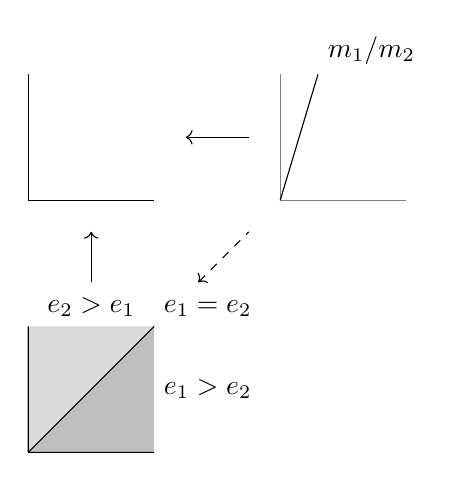
\begin{tikzpicture}[scale=0.8]
 \draw (0,0) -- (0,2)  (0,0)--(2,0);
 \draw[->] (1,-1.3) -- (1,-.5);
 \fill[gray!30] (0,-4) -- (0,-2) -- (2,-2) -- (0,-4);
 \fill[gray!50] (0,-4) -- (2,-4) -- (2,-2) -- (0,-4);
 \draw (0,-4) -- (0,-2) (0,-4) -- (2,-4) (0,-4) -- (2,-2) node[above right]{$e_1=e_2$};
 \draw (1,-2) node[above]{$e_2>e_1$} (2,-3) node[right]{$e_1>e_2$};
 \draw[<-] (2.5,1)--(3.5,1);
 \draw[gray!=30] (4,0) -- (4,2)  (4,0)--(6,0);
 \draw (4,0) -- (4.6,2) node[above right]{$m_1/m_2$};
 \draw[<-,dashed] (2.7,-1.3)--(3.5,-.5);
\end{tikzpicture}
\end{center}
So e.g. the factorisation exists for the subcone $e_2>e_1$ only when $m_1>m_2$, which is compatible with the fact that $\mathbb N^2=Q_{\rm{min}}^{\rm{prestable}}\to Q_{\rm{min}}^{\rm{log.map}}=\mathbb N$ is given by
$e_1\mapsto m_2, e_2\mapsto m_1.$
\end{example}

In fact we plan to work around the problem by directly looking at the desingularisation of the main component of Kim's moduli space of logarithmic maps to expanded targets. We do so because on one hand we are able to carry out Gathmann's recursion in the expanded setting (Remark \ref{rmk:expandedGathmann}), and on the other Kim's approach blends nicely the condition for being smoothable as a relative map into that of being a log morphism.

\subsection{Logarithmic maps with expansions, alignments, factorisations} I will recall the basic definitions from \cite{KimLog,ChenDeg}; see also \cite{OlsCurves,AbramovichMarcusWiseComparison}. Kim's moduli space parametrises log morphisms to an expansion, where the target has the nodal+divisorial log structure, and the minimal log structure on the base is locally free, twisted (in the sense that the irreducible elements are allowed to be roots of the smoothing parameters of the nodes in both the source and target), and identifies all the smoothing parameters of the distinguished nodes of $C$ that map to the same component of the singular locus of $X^{\rm{exp}}=W$ (corank condition). Kim's moduli space should be thought of as the saturation of J. Li's moduli space. In the following $\pM_S^{C/S}$ denotes the log structure on $S$ pulled back from the canonical one on the moduli space of prestable curves (i.e. the minimal log structure on $S$ viewed as the base of a family of log smooth curves), and similarly $\pM_S^{W/S}$.

\begin{definition}
 An \emph{extended log twisted expansion} of $(X,Y)$ is a quadruple $(\pi\colon W\to S, \pi_X\colon W\to X, D\subseteq W, \pM_S^{W/S}\to\pM_S)$ such that:
 \begin{enumerate}
  \item $\pi$ makes $W$ into a flat, proper algebraic space over $S$, with fibers at worst nodal in codimension 1, admitting a lifting to a special log morphism $\pi\colon (W,\pM_W^{W/S})\to(S,\pM_S^{W/S})$, such that:
  \begin{enumerate}
   \item $\pM_W^{W/S}$ and $\pM_S^{W/S}$ are locally free log structures;
   \item for every geometric point $\bar{w}\to W$, either $\bar{w}$ is in the smooth locus of $\pi_S$ and $\pi^\flat\colon \pi^*\overline{\pM}_{S,\bar{w}}^{W/S}\to \overline{\pM}_{W,\bar{w}}^{W/S}$ is an isomorphism, or $\bar{w}$ is in the nodal locus and the following diagram is cocartesian:
   \bcd
   \N\ar[r,"{(1,1)}"]\ar[d,"h"]\ar[dr,phantom,"\lrcorner"] & \N^2\ar[d] \\
   \pi^*\overline{\pM}_{S,\bar{w}}^{W/S}\ar[r] & \overline{\pM}_{W,\bar{w}}^{W/S}
   \ecd
   with $h(1)$ irreducible;
   \item for every geometric point $\bar{s}\to S$ there is a bijection between the irreducible elements of $\overline{\pM}_{S,\bar{s}}^{W/S}$ and the irreducible components of $W_{\bar{s}}^{\text{sing}}$.
  \end{enumerate}
  \item $D\subseteq W$ is a Cartier divisor, smooth over $S$, and such that $\pi_X(D)=Y$;
 \item $\pM_S$ is twisted by integers $(r_1,\ldots,r_l)$ and expanded with respect to $\pM_S^{W/S}$, namely \'{e}tale locally at every point $s\in S$ the morphism of log structures $\pM_S^{W/S}\to\pM_S$ admits a chart:
 \bcd
 \N^l\ar[d]\ar[r,"{(r_1,\cdots,r_l)}"] &\N^l\ar[r,"{(id,0)}"]&\N^l\oplus\N^k\ar[d] \\
 \pM_S^{W/S}\ar[rr] & & \pM_S
 \ecd
  
 \end{enumerate}
\end{definition}
 The log structure on $W$ is then given by
 \[ \pM_W=\pi^*\pM_S\oplus_{\pi^*\pM_S^{W/S}}\pM_W^{W/S}\oplus_{\OO^*_W}\pM^D\]
 where $\pM^D$ is the divisorial log structure associated to $D$. 
Notice that with this definition $(W,\pM_W)\to(S,\pM_S)$ is log smooth.

Similarly a \emph{log twisted curve} is $((C,p_1,\ldots,p_n)\to S, \pM_S^{C/S}\to\pM_S)$ with
\[\pM_C=\pi^*\pM_S\oplus_{\pi^*\pM_S^{C/S}}\pM_C^{C/S}\oplus_{\OO^*_C}\bigoplus_{i=1}^n\pM^{p_i}\]
A log twisted curve is \emph{minimal} if the log structure $\pM_S$ is locally free, and for every geometric point $\bar{s}\to S$ and irreducible element $b\in\overline{\pM}_S$, we can find an irreducible $a\in\overline{\pM}^{C/S}_S$ and a positive integer $l$ such that $a\mapsto lb$ (by definition this means that the morphism of log structures $\pM_S^{C/S}\to\pM_S$ is \emph{simple}).

Finally, fix an $n$-tuple of non-negative contact orders $(c_1,\ldots,c_n)$.
\begin{definition}
 A \emph{relative log prestable map} with tangency condition $\mathbf{c}$ is given by a diagram of log morphisms:
 \bcd
 ((C,\mathbf p),\pM_C)\ar[rr,"f"]\ar[dr] & & ((W,D),\pM_W)\ar[rr,"\pi_X"]\ar[dl] & & (X,Y)\times S \\
  & (S,\pM_S) & & &
 \ecd
 \begin{enumerate}
  \item $((C,\mathbf p),\pM_C)\to (S,\pM_S)$ is a minimal log twisted curve; $((W,\pM_W)\to (S,\pM_S), \\ (W,D)\to(X,Y))$ is an extended twisted log expansion of $(X,Y)$;
  \item (\emph{corank condition}) for every geometric point $\bar{s}\in S$, the rank of \[\operatorname{Coker}(\pM^{W/S}_{S,\bar{s}}\to \pM_{S,\bar{s}})\] is equal to the number of non-distinguished nodes of $C_{\bar{s}}$; recall that a node of $C_{\bar{s}}$ is \emph{distinguished} if it is mapped under $f$ to the singular locus of $W_{\bar{s}}$.
  \item (\emph{log admissibility}) the morphism of log structures $f^\flat\colon f^*\pM_W\to\pM_C$ is simple at every distinguished node;
  \item (\emph{tangency condition}) the underlying map $\underline{f}\colon C\to (W,D)$ is non-degenerate, namely no component of $C$ is mapped entirely into $D$, and locally around every marking $p_i$ we can find a chart
  \bcd
  \N\ar[r,"\cdot c_i"]\ar[d] & \N\ar[d] \\
  f^*\pM^D\ar[r] & \pM^{p_i}
  \ecd
  for the restriction of $f^\flat$ to the $f^*\pM^D$ factor.
  \end{enumerate}
\end{definition}
\begin{definition}
 A relative log prestable map as above is \emph{stable} if for every geometric point $\bar{s}\in S$ the group of automorphisms $(\sigma,\tau)$ is finite, where:
 \begin{enumerate}
  \item $\sigma$ is an automorphism of $((C,\pM_C)\to (S,\pM_S))_{\bar{s}}$ preserving the markings $\mathbf p$;
  \item $\tau$ is an automorphism of $((W,\pM_W)\to (S,\pM_S))_{\bar{s}}$ preserving $D$ and $\pi_X\colon W_{\bar{s}}\to X$;
  \item $\tau\circ f_{\bar{s}}=f_{\bar{s}}\circ \sigma$.
 \end{enumerate}
\end{definition}
\begin{rmk}
 The corank and simplicity condition imply the following: the rank of the locally free log structure $\pM_S$ at $\bar{s}$ amounts to the number of irreducible components of $W_{\bar{s}}^{\text{sing}}$ plus the number of non-distinguished nodes of $C_{\bar{s}}$; all the smoothing parameters of the distinguished nodes mapping to the same component of $W_{\bar{s}}^{\text{sing}}$ are identified \emph{up to twisting}. Indeed, at a distinguished node $q$ of $C$, letting $R$ be the local ring of $S$ at $\pi(q)$, we can find \'{e}tale local charts
 \bcd
 \N^2\oplus_{\N} \pM_{S}\ar[r,"{(id,\cdot m_q)}" below]\ar[d] & \N^2\oplus_{\N} \pM_{S}\ar[d] \\
 f^*\pM_W \ar[r,"f^\flat" below]\ar[d] & \pM_C\ar[d] \\
 R[z_1,\ldots,z_{\dim(X)-1},x,y]/(xy-t)\ar[r,"\left(\substack{x\mapsto a^{m_q}\\ y\mapsto b^{m_q}\\ t\mapsto s^{m_q}}\right)" below=.2cm] & R[a,b]/(ab-s)
 \ecd
 where the twist at $f(q)$ is given by $l$, the one at $q$ is given by $r_q$, and the equality $l=r_qm_q$ must be satisfied.
\end{rmk}
The following is a variation on \cite[\S 3.3]{RSPW2}. I will focus on the case of $(\PP^N|H)$.
\begin{definition}
 Let $(C,\mathbf p)\to (W,D)$ be a radially aligned Kim's log map to $(\PP^N|H)$, and let $\varphi\colon \plC\to\mathbb R_{\geq 0}$ be its tropicalisation, with circuit $\plC_0$. If $\varphi$ does not contract the circuit, set the contraction radius $\delta_f=0$. Otherwise let $\delta_f$ be the minimal distance from the circuit to a vertex supporting a flag that is not contracted by $\varphi$.
\end{definition}
To every Kim's log map we can associate an ordinary (not expanded) log map by collapsing the target and stabilising the curve \cite[Proposition 6.1]{GrossSiebertLog}. Furthermore, by choosing generic hyperplanes that meet the image of the curve transversally at smooth points of the latter, and by pulling back to $C$ the resulting (toric) log structure on $\PP^N$, we may lift any log map to $(\PP^N|H)$ to one to $(\PP^N|\Delta)$, where $\Delta$ denotes the toric boundary of $\PP^N$. Notice that, when looking at the tropicalisation, any generic choice of hyperplanes will add flags only to vertices that already have a non-contracted flag, hence the resulting $\delta_f^{\Delta}$ is the same as $\delta_f$, and does not depend on this choice.

It is discussed in \cite[Proposition 2.4.2.1]{RSPW2} how log morphisms from an fs log scheme $C\to Z$, where $Z$ is a toric variety with the log structure associated to its boundary, are equivalent to the data of $M\xrightarrow{\alpha} H^0(C,\pM_C^{\rm{gp}})$, such that for every $x\in C$ we can find a cone $\sigma$ in the fan of $Z$ and a factorisation:
\bcd
M\ar[r] & H^0(C,\pM_C^{\rm{gp}})\ar[r] & \overline{\pM}_{C,x}^{\rm{gp}} \\
S_\sigma\cap M\ar[u,hook]\ar[rr,dashed] & & \overline{\pM}_{C,x}\ar[u,hook]
\ecd
where $M$ is the character lattice of the torus $T\subseteq Z$, and $S_\sigma$ is the dual cone of $\sigma$. This is useful because it allows them to impose factorisation of $C\to Z\dashrightarrow \PP^1$ to the Smyth's singularity determined by $\delta_f^\Delta$ without having to modify $Z$ (and $C$, and $S$), see \cite[Definition 3.3.3]{RSPW2}.
\begin{dfn}
 A log map $f\colon C\to Z$ from an aligned curve to a toric variety satisfies the factorisation property for a subtorus $H\subseteq T$ if the associated composition \[M_{T/H}\to M\xrightarrow{\alpha} H^0(C,{\pM}_C^{\rm{gp}})\to H^0(\widetilde{C},\pM_{\widetilde{C}}^{\rm{gp}})\] descends to $M_{T/H}\to H^0(\overline{C},\pM_{\overline{C}}^{\rm{gp}})$, where the modification and contraction $C\leftarrow \widetilde{C}\to \overline{C}$ are determined by the contraction radius $\delta_{\alpha}$, that is the largest distance of a vertex from the circuit such that the line bundle associated to $\bar\alpha$ is trivial on the interior of the circle of radius $\delta_\alpha$.
 
 A map $f\colon C\to Z$ is \emph{well-spaced} if it satisfies factorisation for every subtorus $H\subseteq T$.
\end{dfn}

\begin{dfn}
 Let $\alpha\in\N^n$ be a maximal tangency condition. The space $\VZK{\alpha}{\PP^N|H}{d}$ parametrises Kim's log maps from an aligned curve to an expansion such that the associated log map to $(\PP^N|\Delta)$ (for any generic choice of hyperplanes $H_1,\ldots,H_N$) satisfies well-spacedness.
\end{dfn}

I claim that this construction provides a desingularisation of the main component of Kim's space in genus one: indeed it includes the locus of maps from a smooth elliptic curve whose image is not contained in $H$, and its smoothness can be argued as follows. The morphism $\VZK{\alpha}{\PP^N|H}{d}\to \VZa{\alpha}{\PP^N|H}{d}$ is toroidal (this can be argued from \cite[Lemma A and \S 4.3]{AbramovichMarcusWiseComparison} and the analogous statement for the universal target). On the other hand, locally we may find $U_{\VZK{\alpha}{\PP^N|\Delta}{d}}\to U_{\VZK{\alpha}{\PP^N|H}{d}}$ which is \'etale by the infinitesimal criterion (lifting is tantamount to deforming the extra hyperplanes $H_1,\ldots,H_n$). We are then reduced to \cite[Theorem 3.5.1]{RSPW2}.

\subsection{Description of the boundary} As in Gathmann's work, there is a line bundle with section that forces the $k$-th marked point to have tangency of order $\alpha_k+1$ to $H$, which in the maximal tangency situation and in the expanded setup (as is the case for us) really forces the target to break, and the $k$-th marking $x_k$ to lie on a non-trivial component mapped to the highest level of the accordion. The line bundle and section $(\mathcal L_{\alpha,k},s_{\alpha,k})$ are the pullback of $(x_k^*\Omega_{C}^{\otimes \alpha_k+1}\otimes\ev_1^*\OO_\PP^N(1),\ev_k^*(d^{\alpha_k+1}s))$ from the collapsed and stabilised map. The description of the boundary in the case of $(\PP^N|H)$ boils down to a dimension computation, and is already present in the work of Vakil \cite{Vre}. There are three relevant combinatorial types, corresponding to bipartite graphs:
\begin{enumerate}[label=(\alph*)]
 \item $\Yagraph$ \begin{multline*}\mathcal Y^a=\left(\VZ{\alpha^{(1)}\cup\{m^{(1)}\}}{\PP^N|H}{d_1}\times\prod_{i=2}^r\M{0}{\alpha^{(i)}\cup\{m^{(i)}\}}{\PP^N|H}{d_i}\right)\times_{H^r} \\ \M{0}{(-m^{(1)},\ldots,-m^{(r)})\cup\alpha^{(0)}}{\PP_H(\OO\oplus\OO(1)}{d_0}^\thicksim\end{multline*}
 \item $\Ybgraph$ \begin{multline*}\mathcal Y^b=\left(\M{0}{\alpha^{(1)}\cup\{m^{(1)},m^{(2)}\}}{\PP^N|H}{d_1}\times\prod_{i=3}^r\M{0}{\alpha^{(i)}\cup\{m^{(i)}\}}{\PP^N|H}{d_i}\right)\times_{H^r}\\ \M{0}{(-m^{(1)},-m^{(2)}\ldots,-m^{(r)})\cup\alpha^{(0)}}{\PP_H(\OO\oplus\OO(1)}{d_0}^\thicksim\end{multline*}
 \item $\Ycgraph$\begin{multline*}\mathcal Y^c= \prod_{i=1}^r\M{0}{\alpha^{(i)}\cup\{m^{(i)}\}}{\PP^N|H}{d_i}\times_{H^r}\VZdrc{(-m^{(1)},\ldots,-m^{(r)})\cup\alpha^{(0)}}{\PP_H(\OO\oplus\OO(1)}{d_0}^\thicksim\end{multline*}
\end{enumerate}
A few remarks on the notation are in order: a white circle in the graphs always stands for a genus one component; the tilde denotes moduli spaces of rubber maps, which were introduced in \cite{GraberVakil} (material on how they compare to the ordinary moduli space of maps to the underlying $H$ can be found in \cite[Chapter 5]{GathmannThesis}). DRC stands for ``double ramification cycle'', i.e. for the extra equation in $\Pic$ that needs to be satisfied:
\[f_{|E}^*\mathcal O_H(1)\cong\mathcal O_E\left(\sum_{x_j\in E}\alpha_jx_j-\sum_{i=1}^r m^{(i)}y_i\right).\]
In the genus one case, this is a divisorial condition. When the left hand side is trivial, e.g. when $H=\{\infty\}\subseteq \PP^1$, an explicit tautological formula was already known to R. Hain \cite{Hain} (later confirmed and generalised in \cite{JPPZ}). What we can do exploiting Gathmann's argument is computing (relating) a number of $\psi$-integrals against the DRC, more in the spirit of \cite{BSZ}.

It is worth subdividing case (c) above into $\mathcal Y^c_+$ (for $d_0>0$) and $\mathcal Y^c_0$ (for $d_0=0$): notice that the generic element of the latter is already aligned (indeed the minimal monoid is $\N$, since all the nodes are distinguished and map to the same component of the singular locus of the target); on the other hand we need to impose the well-spacedness condition, which will hopefully be expressible as a tautological integral, by expanding on the analysis of Lemma \ref{lem:fundamental}. The data above depend on a splitting $(A,B,M)$ of the markings, degree, and external multiplicities, such that $d_0+\sum m^{(i)}=\sum A^{(0)}$, and factorisation should impose $N-1$ independent conditions, unless all the $m^{(i)}\geq 2$, in which case there are only $N-2$ conditions (this would be the dimensionally relevant case). Finally, let me observe that all the insertions that we are interested in are pulled back from the moduli space of maps to the collapsed target, hence any locus with positive-dimensional fibers for the collapsing may be overlooked; this is the case when there is more than one non-trivial component mapping to higher level in the accordion, which is the reason why only the three graph types above appear. All the boundary divisors appear in the vanishing locus of $s_{\alpha,k}$ with positive multiplicity $\frac{m^{(1)}\cdots m^{(r)}}{r!}$ (the $r!$ is only there to make the gluing nodes unordered), as already predicated in \cite{Vre} and discussed in Remark \ref{rmk:expandedGathmann}.

The formula in the case of non-maximal tangency can be proven by adding $h=d-\sum\alpha$ auxiliary markings of multiplicity $(1,\ldots,1)$, and then forgetting them (which is generically an $h!\colon 1$ cover), pretty much along the lines of \cite[Corollary 3.5]{Ga}. Importantly, the difference between $\psi_k$ on the space with auxiliary markings and $\fgt_{n+1,\ldots,n+h}^*\psi_k$ can be expressed in terms of boundary classes. It may be useful to notice that as soon as there is more than one non-trivial component at higher level, or the only such component has zero horizontal degree and contains more than one of the auxiliary markings, then the corresponding locus has positive-dimensional fibers for forgetting $x_{n+1},\ldots,x_{n+h}$ and collapsing. Also, forgetting a point on the genus one component at level one in case (c) may make the difference between having to impose the DRC condition or not. So after all the general formula takes the following shape:
\begin{multline*}(\alpha_k\psi_k+\ev_k*H)\cap[\VZ{\alpha}{\PP^N|H}{d}]=[\VZ{\alpha+e_k}{\PP^N|H}{d}]+\\ \sum_{(I)}[\mathcal Y_a]+\sum_{(I)}[\mathcal Y_b]+\sum_{(I)}[\mathcal Y_c]+\sum_{(II)}[\mathcal Y_c^{\rm{no DRC}}]\end{multline*}
where $(I)$ and $(II)$ range over all the splittings $(A,B,M)$ such that $\alpha_k\in A^{(0)}$ and
\begin{enumerate}[label=(\Roman*)]
 \item $d_0+\sum m^{(i)}=\sum A^{(0)}$,
 \item $d_0+\sum m^{(i)}=\sum A^{(0)}+1$.
\end{enumerate}

\subsection{Sample computations} I will exemplify the use of the recursion in some low-dimensional situations. Let me introduce the following shorthand notation: I will write $H_k$ for $\ev_k^* H$ and $\psi_k^{\{n_1,\ldots,n_h\}}$ for $\fgt_{\{n_1,\ldots,n_h\}}^*\psi_k$.
\begin{ex}
 Consider the following step of the recursion:
 \begin{multline*} (2\psi_1+H_1)\cdot [\VZ{(2,0)}{\PP^1|\infty}{2}]=\\ 2\ {\tikz[baseline=-3pt,scale=.7]{
\draw (2,0) node[above]{$\{x_1,x_2\}$} -- (0,0)node[below]{$d=2$};
\draw (2,0) circle(2pt)[fill=black];
\draw (0,0) circle(2pt)[fill=white];
\draw (-1,1.5) -- (1,1.5) -- (1,-1.5) -- (-1,-1.5) -- (-1,1.5);
\draw (1,1.5) -- (3,2) -- (3,-1) -- (1,-1.5);
}}+
{\tikz[baseline=-3pt,scale=.7]{
\draw (2,0) node[above]{$\{x_1\}$} to[out=210,in=-30] (0,0)node[above]{$\{x_2\}$}node[below=.15cm]{$d=2$} (2,0) -- (0,0);
\draw (2,0) circle(2pt)[fill=black];
\draw (0,0) circle(2pt)[fill=black];
\draw (-1,1.5) -- (1,1.5) -- (1,-1.5) -- (-1,-1.5) -- (-1,1.5);
\draw (1,1.5) -- (3,2) -- (3,-1) -- (1,-1.5);
}}+
2\ {\tikz[baseline=-3pt,scale=.7]{
\draw (2,0) node[above]{$\{x_1\}$} -- (0,0)node[above]{$\{x_2\}$}node[below]{$d=2$};
\draw (2,0) circle(2pt)[fill=white];
\draw (0,0) circle(2pt)[fill=black];
\draw (-1,1.5) -- (1,1.5) -- (1,-1.5) -- (-1,-1.5) -- (-1,1.5);
\draw (1,1.5) -- (3,2) -- (3,-1) -- (1,-1.5);
}}+
{\tikz[baseline=-3pt,scale=.7]{
\draw (2,0) node[above]{$\{x_1\}$} -- (0,.5)node[above]{$d=1$} (2,0)--(0,-.5)node[below]{$d=1$};
\draw (2,0) circle(2pt)[fill=white];
\draw (0,0.5) circle(2pt)[fill=black] (0,-0.5) circle(2pt)[fill=black];
\draw (-1,1.5) -- (1,1.5) -- (1,-1.5) -- (-1,-1.5) -- (-1,1.5);
\draw (1,1.5) -- (3,2) -- (3,-1) -- (1,-1.5);
}}
\end{multline*}
Notice that in the $\mathcal Y_a$ term $x_2$ has to be at level one to ensure stability (yet this results in a positive dimensional moduli space with no insertions at level zero, so this term will never contribute to the invariants); in the $\mathcal Y_b$ and in the first $\mathcal Y_c$ term it has to be at level zero, otherwise there would be a positive dimensional moduli space with no insertions; while I have remained agnostic as to where $x_2$ lies in the second $\mathcal Y_c$ term. Now choosing $\psi_1\psi_2H_2$ as insertion, we see that the only contributing term on the right hand side is the first $\mathcal Y_c$ term, so we get the following equality:
\[\langle \psi(2\psi +H),\psi H\rangle^{\PP^1|\infty,\rm{red}}_{1,(2,0),2}=2\langle \psi H,1\rangle^{\PP^1|\infty}_{0,(2,0),2}\langle\psi,1\rangle^{\rm{DRC}}_{1,(-2,2)}\]
The next step of the recursion involves an auxiliary marking $x_3$. Knowing the insertion, the only non-trivial contributions are
 \begin{multline*} (\psi_1+H_1)\cdot [\VZ{(1,0,1)}{\PP^1|\infty}{2}]= 2\ {\tikz[baseline=-3pt,scale=.7]{
\draw (2,0) node[above]{$\{x_1,x_3\}$} -- (0,0)node[above]{$\{x_2\}$} node[below]{$d=2$};
\draw (2,0) circle(2pt)[fill=black];
\draw (0,0) circle(2pt)[fill=white];
\draw (-1,1.5) -- (1,1.5) -- (1,-1.5) -- (-1,-1.5) -- (-1,1.5);
\draw (1,1.5) -- (3,2) -- (3,-1) -- (1,-1.5);
}}+
2\ {\tikz[baseline=-3pt,scale=.7]{
\draw (2,0) node[above]{$\{x_1,x_3\}$} -- (0,0)node[above]{$\{x_2\}$} node[below]{$d=2$};
\draw (2,0) circle(2pt)[fill=white];
\draw (0,0) circle(2pt)[fill=black];
\draw (-1,1.5) -- (1,1.5) -- (1,-1.5) -- (-1,-1.5) -- (-1,1.5);
\draw (1,1.5) -- (3,2) -- (3,-1) -- (1,-1.5);
}}+\ldots
\end{multline*}

By comparing $\psi_1$ with $\psi_1^{\{3\}}$ on the left hand side, a term appears cancelling with the $\mathcal Y_a$ on the right hand side; after forgetting $x_3$, we recognise $\VZ{(2,0)}{\PP^1|\infty}{2}$ in the latter. Also, the $\mathcal Y_c$ term has no DRC condition. By substituting in the above we get:
\[\langle \psi(2\psi +H)(\psi+H),\psi H\rangle^{\PP^1|\infty,\rm{red}}_{1,(1,0),2}=2\langle \psi H,1\rangle^{\PP^1|\infty}_{0,(2,0),2}\left(\langle\psi,1\rangle^{\rm{DRC}}_{1,(-2,2)}+\langle2\psi^2,1\rangle_{1,2}\right)\]
Finally
\[H_1\cdot[\VZ{(0,0,1,1)}{\PP^1|\infty}{2}]={\tikz[baseline=-3pt,scale=.7]{
\draw (2,.5) node[above]{$\{x_1,x_i\}$} -- (0,0)node[above]{$\{x_2\}$} node[below]{$d=2$}  (2,-.5)node[above]{$\{x_{7-i}\}$} -- (0,0);
\draw (2,.5) circle(2pt)[fill=black];
\draw (2,-.5) circle(2pt)[fill=black];
\draw (0,0) circle(2pt)[fill=white];
\draw (-1,1.5) -- (1,1.5) -- (1,-1.5) -- (-1,-1.5) -- (-1,1.5);
\draw (1,1.5) -- (3,2) -- (3,-1) -- (1,-1.5);
}} (i=3,4) +\ldots\]
from which, forgetting $\{x_3,x_4\}$ and substituting, we get:
\[\langle \psi(2\psi +H)(\psi+H)H,\psi H\rangle^{\PP^1,\rm{red}}_{1,2,2}=2\langle \psi H,1\rangle^{\PP^1|\infty}_{0,(2,0),2}\left(\langle\psi,1\rangle^{\rm{DRC}}_{1,(-2,2)}+\langle2\psi^2,1\rangle_{1,2}\right)\]
It is easy to see from the discussion at the end of Section \ref{sec:redinv} that the reduced invariant on the left hand side coincides with the ordinary one, since the boundary does not contribute in this case. The left hand side, as well as the genus zero relative invariant on the right hand side, can be computed using Gathmann's software GROWI; the right hand side can be computed using the string and dilaton equations, together with the genus one DRC formula of \cite[\S 0.5.2]{JPPZ} with $A=(-2,2)$:
\[\operatorname{DR}_1(A)=\frac{1}{2}\left(\sum_{i=1}^n a_i^2\psi_i-\sum_{I\subseteq [n],\lvert I\rvert\geq2}a_I^2\delta_I-\frac{1}{12}\xi_*[\oM_{0,n+2}]\right)\]
where $A$ is a zero-sum $n$-tuple of integers, $a_I=\sum_{i\in I}a_i$, and $\delta_I=\delta_{0,I|1,I^c}$.
\end{ex}

It may seem hopeless to exploit the recursion to compute the invariants of $H$ in terms of those of $\PP^N$, because degree $d$, genus one invariants of $H$ will appear both at the $d$-th and at the $(d+1)$-st step of the recursion, but in the latter they will come mingled in a range of admissible DRC conditions. Instead writing invariants of $H$ as one well-chosen DRC integral seems to be the key to success.
\begin{ex}
 Assume we want to compute $\psi_1^5\cdot[\VZ{1}{\PP^1}{2}]$ by thinking of $\PP^1$ as a line in $\PP^2$ and applying the recursion. There is a $4:1$ cover of $\VZ{1}{\PP^1}{2}$ by $\VZ{(0,2)}{\PP^2|H}{2}^\thicksim$, forgetting the second marking. Hence we may start from
 \[
 H_1\cdot[\VZ{(0,2)}{\PP^2|H}{2}]=
 2{\tikz[baseline=-3pt,scale=.7]{
\draw (2,0) node[above]{$\{x_1,x_2\}$} -- (0,0)node[above]{$d=2$};
\draw (2,0) circle(2pt)[fill=black];
\draw (0,0) circle(2pt)[fill=white];
\draw (-1,1.5) -- (1,1.5) -- (1,-1.5) -- (-1,-1.5) -- (-1,1.5);
\draw (1,1.5) -- (3,2) -- (3,-1) -- (1,-1.5);
}}+
{\tikz[baseline=-3pt,scale=.7]{
\draw (2,0) node[above,align=center]{$d=2$,\\$\{x_1,x_2\}$};
\draw (2,0) circle(2pt)[fill=white];
\draw (-1,1.5) -- (1,1.5) -- (1,-1.5) -- (-1,-1.5) -- (-1,1.5);
\draw (1,1.5) -- (3,2) -- (3,-1) -- (1,-1.5);
}}+\ldots
 \]
by multiplying both sides with $(\psi_1^{\{2\}})^5$ and rearranging we obtain:
\[\langle \psi^5\rangle^{\PP^1,\rm{red}}_{1,1,2}=\frac{1}{4}(\psi_1^{\{2\}})^5H_1[\VZ{(0,2)}{\PP^2|H}{2}]-\frac{1}{2}\psi_1^5[\VZ{(2)}{\PP^2|H}{2}]\]
 Applying the recursion again to the terms on the right hand side we get:
 \begin{multline*}\frac{1}{4}(\psi_1^{\{2\}})^5H_1[\VZ{(0,2)}{\PP^2|H}{2}]=\frac{1}{4}(\psi_1^{\{2,3\}})^5H_1(\psi_2^{\{3\}}+H_2)[\VZ{(0,1,1)}{\PP^2|H}{2}]\\ -\frac{1}{4}(\psi_1^{\{2\}})^5H_1[\VZ{(1,1)}{\PP^2|H}{2}]\end{multline*}
 \begin{multline*}-\frac{1}{2}\psi_1^5[\VZ{(2)}{\PP^2|H}{2}]=-\frac{1}{2}(\psi_1^{\{2\}})^5(\psi_1^{\{2\}}+H_1)[\VZ{(1,1)}{\PP^2|H}{2}]\\+\frac{1}{2}(\psi_1^{\{2\}})^5[\VZ{(1,1)}{\PP^2|H}{2}^\thicksim]\end{multline*}
 Notice that the last term appearing reduces to $\frac{1}{2}\langle \psi^5\rangle^{\PP^1,\rm{red}}_{1,1,2}$; luckily the scalar factor is not the same as in the left hand side above. So we get
 \begin{multline*}
  \frac{1}{2}\langle \psi^5\rangle^{\PP^1,\rm{red}}_{1,1,2}=\frac{1}{4}(\psi_1^{\{2,3\}})^5H_1(\psi_2^{\{3\}}+H_2)[\VZ{(0,1,1)}{\PP^2|H}{2}] \\ -\frac{1}{4}(\psi_1^{\{2\}})^5(2\psi_1^{\{2\}}+3H_1)[\VZ{(1,1)}{\PP^2|H}{2}]
 \end{multline*}
After further manipulations using $\psi_1^{\{2\}}=\psi_1-D_{1,2}$ we rewrite the right hand side as:
\[\frac{1}{4}\langle\psi^5H,(\psi+H)H\rangle^{\PP^2,\rm{red}}_{1,2,2}-\frac{1}{4}\langle\psi^4H(\psi+H)H\rangle^{\PP^2,\rm{red}}_{1,1,2}-\frac{1}{4}\langle\psi^5(2\psi+3H)H\rangle^{\PP^2,\rm{red}}_{1,1,2}\]
According to the formulae at the end of Section \ref{sec:redinv}, the relation with ordinary invariants is the following:
\begin{align*}
 \langle\psi^5H,\psi H\rangle^{\PP^2,\rm{red}}_{1,2,2}&=\langle\psi^5H,\psi H\rangle^{\PP^2}_{1,2,2}+\frac{1}{24}\langle\psi^5H,\psi H,1\rangle^{\PP^2}_{0,3,2}-\langle\psi,\psi\rangle_{1,2}\langle\psi^5H,\psi H\rangle^{\PP^2}_{0,2,2}\\
 \langle\psi^5H,H^2\rangle^{\PP^2,\rm{red}}_{1,2,2}&=\langle\psi^5H, H^2\rangle^{\PP^2}_{1,2,2}+\frac{1}{24}\langle\psi^5H, H^2,1\rangle^{\PP^2}_{0,3,2}
\end{align*}
\noindent etc. where the first correction terms comes from $\oM_{1,1}\times\M{0}{n+1}{\PP^2}{2}$ (with obstruction bundle $-\lambda_1$ on the first factor), and the second correction term (only relevant when computing the first of the invariants) comes from $\oM_{1,2}\times\M{0}{2}{\PP^2}{2}$. Instead $\langle \psi^5\rangle^{\PP^1,\rm{red}}_{1,1,2}=\langle \psi^5\rangle^{\PP^1}_{1,1,2}$ because $\psi$ appears to the power $5$ while on the boundary we find $\oM_{1,2}$ at most. Again the equality can be checked using GROWI.
\end{ex}

You may be worried that it was just a lucky coincidence that the integral we were interested in appeared on different sides of the equality with different coefficients, instead it seems to be a general feature.
\begin{rmk}
 Assume we want to compute $\langle\tau_{h_1}H^{k_1},\ldots,\tau_{h_1}H^{k_1}\rangle^{\PP^{N-1},\rm{red}}_{1,n,d}$ by writing it as $\frac{1}{d^2}(\psi_1^{\{n+1\}})^{h_1}H^{k_1}\cdots(\psi_n^{\{n+1\}})^{h_n}H^{k_n}\cdot[\VZ{(0,\ldots,0,d)}{\PP^N|H}{d}^\thicksim]$. Let me start from the recursion step $H_1\cdot[\VZ{(0,\ldots,0,d)}{\PP^N|H}{d}]=\ldots:$
 
 \begin{description}
  \item[$\mathcal Y_a$] $d{\tikz[baseline=-3pt,scale=.7]{
\draw (2,0) node[above]{$\{x_1,x_{n+1}\}$} -- (0,0)node[above]{$d$};
\draw (2,0) circle(2pt)[fill=black];
\draw (0,0) circle(2pt)[fill=white];
\draw (-1,1.5) -- (1,1.5) -- (1,-1.5) -- (-1,-1.5) -- (-1,1.5);
\draw (1,1.5) -- (3,2) -- (3,-1) -- (1,-1.5);
}}$ contributes $\frac{1}{d}\psi_1^{h_1}H^{k_1}\cdots\psi_n^{h_n}H^{k_n}\cdot[\VZ{(d,\ldots,0)}{\PP^N|H}{d}]$; if the curve configuration is this, while there is any other marking at level one, then $\fgt_{n+1}$ has positive dimensional fibers; otherwise there must be another component of positive horizontal degree (these contribution are computed inductively on $d$);
\item[$\mathcal Y_b$] is an entirely rational story;
\item[$\mathcal Y_c$] {\tikz[baseline=-3pt,scale=.7]{
\draw (2,0) node[above,align=center]{$d$,\\$\{x_1,\ldots,x_{n+1}\}$};
\draw (2,0) circle(2pt)[fill=white];
\draw (-1,1.5) -- (1,1.5) -- (1,-1.5) -- (-1,-1.5) -- (-1,1.5);
\draw (1,1.5) -- (3,2) -- (3,-1) -- (1,-1.5);
}} is the term we are meant to compute, while all other terms will include a DR integral of lower degree.
 \end{description}
I shall look one step further into the recursion for computing $[\VZ{(0,\ldots,0,d)}{\PP^N|H}{d}]$: in order to see this term consider the recursion at $((d-1)\psi_{n+1}+H_{n+1})\cdot[\VZ{(0,\ldots,0,d-1,1)}{\PP^N|H}{d}]$. This produces:
\begin{description}
  \item[$\mathcal Y_a$] $d{\tikz[baseline=-3pt,scale=.7]{
\draw (2,0) node[above]{$\{x_{n+1},x_{n+2}\}$} -- (0,0)node[above]{$d$};
\draw (2,0) circle(2pt)[fill=black];
\draw (0,0) circle(2pt)[fill=white];
\draw (-1,1.5) -- (1,1.5) -- (1,-1.5) -- (-1,-1.5) -- (-1,1.5);
\draw (1,1.5) -- (3,2) -- (3,-1) -- (1,-1.5);
}}$ this is the one we are after; while
$(d-1){\tikz[baseline=-3pt,scale=.7]{
\draw (2,.5) node[above]{$\{x_{k},x_{n+1}\}$} -- (0,0)node[above]{$d$};
\draw (2,-.5) node[above]{$\{x_{n+2}\}$} -- (0,0);
\draw (2,.5) circle(2pt)[fill=black];
\draw (2,-.5) circle(2pt)[fill=black];
\draw (0,0) circle(2pt)[fill=white];
\draw (-1,1.5) -- (1,1.5) -- (1,-1.5) -- (-1,-1.5) -- (-1,1.5);
\draw (1,1.5) -- (3,2) -- (3,-1) -- (1,-1.5);
}}$ gives lower tangency condition $[\VZ{(0,\ldots,d-1,\ldots,0)}{\PP^N|H}{d}]$; and all other terms have lower degree.
\item[$\mathcal Y_c$] {\tikz[baseline=-3pt,scale=.7]{
\draw (2,0) node[above,align=center]{$d$,\\$\{x_1,\ldots,x_{n+1},x_{n+2}\}$};
\draw (2,0) circle(2pt)[fill=white];
\draw (-1,1.5) -- (1,1.5) -- (1,-1.5) -- (-1,-1.5) -- (-1,1.5);
\draw (1,1.5) -- (3,2) -- (3,-1) -- (1,-1.5);
}} has positive dimensional fibers for $\fgt_{n+1,n+2}$, and all other terms have lower degree.
 \end{description}
 Finally let's look one step further into the reduction of $[\VZ{(d,\ldots,0)}{\PP^N|H}{d}]$: we have $((d-1)\psi_1^{n+1}+H_1)\cdot[\VZ{(d-1,\ldots,0,1)}{\PP^N|H}{d}]=\ldots:$
 \begin{description}
  \item[$\mathcal Y_a$] ${\tikz[baseline=-3pt,scale=.7]{
\draw (2,0) node[above]{$\{x_{1},x_{n+1}\}$} -- (0,0)node[above]{$d$};
\draw (2,0) circle(2pt)[fill=black];
\draw (0,0) circle(2pt)[fill=white];
\draw (-1,1.5) -- (1,1.5) -- (1,-1.5) -- (-1,-1.5) -- (-1,1.5);
\draw (1,1.5) -- (3,2) -- (3,-1) -- (1,-1.5);
}}$ is the one we care about;
$(d-1){\tikz[baseline=-3pt,scale=.7]{
\draw (2,.5) node[above]{$\{x_{k},x_{1}\}$} -- (0,0)node[above]{$d$};
\draw (2,-.5) node[above]{$\{x_{n+1}\}$} -- (0,0);
\draw (2,.5) circle(2pt)[fill=black];
\draw (2,-.5) circle(2pt)[fill=black];
\draw (0,0) circle(2pt)[fill=white];
\draw (-1,1.5) -- (1,1.5) -- (1,-1.5) -- (-1,-1.5) -- (-1,1.5);
\draw (1,1.5) -- (3,2) -- (3,-1) -- (1,-1.5);
}}$ has lower number of markings (indeed $\psi_1^{\{n+1\}}$ and $\psi_k^{\{n+1\}}$ restrict to $0$ on this locus, and $\ev_1=\ev_k$); while all other terms have lower degree.
\item[$\mathcal Y_c$] {\tikz[baseline=-3pt,scale=.7]{
\draw (2,0) node[above,align=center]{$d$,\\$\{x_1,\ldots,x_{n+1}\}$};
\draw (2,0) circle(2pt)[fill=white];
\draw (-1,1.5) -- (1,1.5) -- (1,-1.5) -- (-1,-1.5) -- (-1,1.5);
\draw (1,1.5) -- (3,2) -- (3,-1) -- (1,-1.5);
}} contributes $\frac{1}{d}\psi_1^{h_1}H^{k_1}\cdots\psi_n^{h_n}H^{k_n}\cdot[\VZ{(0,\ldots,0,d)}{\PP^N|H}{d}^\thicksim]$ so \emph{there is no cancellation}, while all other terms have lower degree.
 \end{description}
 To sum up, it is possible to determine the reduced genus one restricted invariants of $H$ in terms of those of $\PP^N$ and the genus zero theory, by induction on the degree, number of markings, and total tangency order.
\end{rmk}
The last example is meant to show the factorisation condition in action.
\begin{ex}
 Let me apply the recursion at $x_1$ on $\VZ{(2,0)}{\PP^2|H}{2}$ with insertion $\psi_1\psi_2^2H_2^2$. The only surviving boundary term is of type $\mathcal Y^c_0$ and it is isomorphic to $2\oM^{DRC}_{1,(-2,2)}\times\M{0}{(0,2)}{\PP^2|H}{2}^{\rm{ramif}}$ with $x_1$ sitting in the first factor, and $x_2$ in the second. In this case the factorisation condition is simply asking that the genus zero map is ramified at the second marking: since we already know that $\operatorname{d}\! f_q\colon T_{C,q}\to N_{H/\PP^2,f(q)}$ vanishes, it is enough to require that $\operatorname{d}\! f_q\colon T_{C,q}\to T_{H,f(q)}$ also does. This is the tautological class $\psi_q+2H_q$. Summing up we have:
 \[\langle\psi\rangle^{DRC}_{1,(-2,2)}\langle\psi^2H^2,\psi+2H\rangle^{\PP^2|H}_{0,(0,2),2}=\langle\psi(2\psi+H),\psi^2H^2\rangle^{\PP^2|H,\rm{red}}_{1,(2,0),2}\]
 Applying the recursion twice more we may rewrite the right hand side as
 \[\langle\psi(2\psi+H)(\psi+H)H,\psi^2H^2\rangle^{\PP^2,\rm{red}}_{1,2,2}-2\langle2\psi^2\rangle_{1,2}\langle\psi^2H^2,\psi+2H\rangle^{\PP^2|H}_{0,(0,2),2}\]
 Finally
\begin{multline*}
 \langle\psi(2\psi+H)(\psi+H)H,\psi^2H^2\rangle^{\PP^2,\rm{red}}_{1,2,2}=\langle\psi(2\psi+H)(\psi+H)H,\psi^2H^2\rangle^{\PP^2}_{1,2,2}+\\ \frac{1}{24}\langle1,\psi(2\psi+H)(\psi+H)H,\psi^2H^2\rangle^{\PP^2}_{0,3,2}-\frac{3}{24}\langle\psi H^2,\psi^2H^2\rangle^{\PP^2}_{0,2,2}+\\
 -\frac{1}{24}\langle\psi H(3\psi H+2\psi^2),\psi H^2\rangle^{\PP^2}_{0,2,2}
\end{multline*}
where the last three terms are the boundary corrections \[{\tikz[baseline=-3pt]{
\draw (0,0)node[above left]{$\psi-2\lambda_1$} -- (1,0)node[above right]{$\{x_1,x_2\}$};
\draw (0,0) circle(2pt)[fill=white];
\fill (1,0) circle (2pt)}
}+ {\tikz[baseline=-3pt]{
\draw (0,0)node[below]{$\{x_1\}$} -- node[above right]{$\psi$}(1,0)node[below]{$\{x_2\}$};
\draw (0,0) circle(2pt)[fill=white];
\fill (1,0) circle (2pt)}
}+ {\tikz[baseline=-3pt]{
\draw (0,0)node[below]{$\{x_2\}$} -- node[above right]{$\psi$}(1,0)node[below]{$\{x_1\}$};
\draw (0,0) circle(2pt)[fill=white];
\fill (1,0) circle (2pt)}
}
\]
\end{ex}







%%%%%%%%%%%%%%%%%%%%%%%%%%%%%%%%%%%%%%%%%%%%%%%%%
%\backmatter %d'ora in poi sono nel'ultima parte della tesi


\cleardoublepage
%\phantomsection
\addcontentsline{toc}{chapter}{Bibliography}
\bibliographystyle{alpha}
\bibliography{the}



%\printindex %stampa l'indice analitico. ricordarsi di compilare anche MakeIndex

\addtocontents{toc}{\protect\setcounter{tocdepth}{-1}} %d'ora in poi nascondo tutti i capitoli e tutte le sezioni



%\begin{comment}

%\chapter*{Ringraziamenti}



%\end{comment}

%\addtocontents{toc}{\protect\setcounter{tocdepth}{1}}

\end{document}